\documentclass[a4paper,12pt]{report}

%%%%%%%%%%%%%%%%%%%%%%%%%%%%%%%%%%%%%%%%%%%%%%%%%%%%%%
% packages... 
\usepackage[utf8]{inputenc}
\usepackage[italian]{babel}

\usepackage[hyphens]{url}
\usepackage[backend=bibtex]{biblatex}

\usepackage{listings}
% Per generare il file PDF aderente alle specifiche PDF/A-1b. Verificarne poi la validità. 
%\usepackage[a-1b]{pdfx}
\usepackage{hyperref}
\usepackage{graphicx}
\usepackage{csquotes}
\usepackage{color, colortbl}
% usato per codice
\usepackage{courier}

\usepackage{todonotes}
\usepackage{refcheck}

% draft più leggibile
\usepackage[a4paper,top=2cm,bottom=2cm,outer=5cm,verbose,headheight=1cm,heightrounded]{geometry}
\setlength{\marginparwidth}{4.5cm} %per farci stare todonotes

\definecolor{CodeGray}{gray}{0.95}
\definecolor{TableGray}{gray}{0.9}
\definecolor{LightTextColor}{rgb}{0.5,0.5,0.5}

\lstloadlanguages{Python}
\lstnewenvironment{code}[1][]%
{
   \noindent
   \minipage{\linewidth} 
   \vspace{0.5\baselineskip}
   \lstset{
        language=Python,
        basicstyle=\ttfamily\footnotesize,
        numbers=left,                           % where to put the line-numbers
        numberstyle=\ttfamily\footnotesize,     % the size of the fonts that are used for the line-numbers
        stepnumber=1,                           % the step between two line-numbers. If it is 1 each line will be numbered
        numbersep=5pt,                          % how far the line-numbers are from the code
        backgroundcolor=\color{CodeGray},       % choose the background color. You must add \usepackage{color}
        showspaces=false,                       % show spaces adding particular underscores
        showstringspaces=false,                 % underline spaces within strings
        showtabs=false,                         % show tabs within strings adding particular underscores
        tabsize=2,                              % sets default tabsize to 2 spaces
        captionpos=b,                           % sets the caption-position to bottom
        breaklines=true,                        % sets automatic line breaking
        breakatwhitespace=false,                % sets if automatic breaks should only happen at whitespace
        #1}}
{\endminipage}

\newcommand{\columnstyle}[1]{\texttt{#1}}
\newcommand{\filenamestyle}[1]{\texttt{#1}}
\newcommand{\methodstyle}[1]{\textbf{#1}}
\newcommand{\quotestyle}[1]{\textit{#1}}
\newcommand{\engstyle}[1]{\textbf{#1}}

\def\light#1{{\color{LightTextColor}#1}}
\newcommand{\skipline}{\vspace{0.2in}}
\newcommand{\lighttext}[1]{\skipline\noindent\light{\texttt{#1}}\skipline}

% \bibliography{Biblio}
\addbibresource{Biblio.bib}

%%%%%%%%%%%%%%%%%%%%%%%%%%%%%%%%%%%%%%%%%%%%%%%%%%%%%
\begin{document}

% Frontespizio
\begin{titlepage}
\begin{center}

\includegraphics[width=\textwidth]{Logo.jpg}\\
{\large{\bf Corso di Laurea Triennale in Informatica}}
\end{center}
\vspace{12mm}
\begin{center}
{\huge{\bf Studio sull'incidentalità stradale}}\\
\vspace{4mm}
{\huge{\bf tramite dataset aperti}}\\
\end{center}
\vspace{12mm}
\begin{flushright}
{\large{\bf Tesi di Laurea di:}}\\
{\large{\bf Gabriele Padovani}}\\
{\large{\bf Matr. 909165}}\\
\end{flushright}
\vspace{4mm}
\begin{flushleft}
{\large{\bf Relatore:}}\\
{\large{\bf Andrea Trentini}}\\
\end{flushleft}
\vspace{12mm}
\begin{center}
{\large{\bf Anno Accademico 2020/2021}}
\end{center}
\end{titlepage}

\tableofcontents

\listoftodos

%%%%%%%%%%%%%%%%%%%%%%%%%%%%%%%%%%%%%%%%%%%%%%%%%%%%%%
\chapter{Introduzione}
\todo{lelepado: per andare a capo, per parole come 'interessante', latex sbaglia la separazione in sillabe, che lei sappia devo specificarlo manualmente ogni volta con \\hyphenation?}

Il termine dati aperti, o liberi, tradotto dall'inglese \quotestyle{open data}, 
si riferisce a collezioni di informazioni liberamente accessibili e 
utilizzabili. 

La Open Knowledge Foundation, per definire il concetto di \quotestyle{openness}, 
scrive: 

\begin{quotation}
    Open means anyone can freely access, use, modify, and share for any purpose 
    (subject, at most, to requirements that preserve provenance and openness). \cite{OPENDEFINITION:1}
\end{quotation}

In questa definizione, viene specificato che, chiunque ne sia capace, ha la possibilità di 
fare uso, modificare le informazioni, e condividerle per qualunque scopo. 
Un concetto da evidenziare, sono le possibili restrizioni degli open data, 
di cui si parla nella sezione tra parentesi della citazione, 
cioè l'obbligo di condividere i dati modificati 
mantenendo lo stesso tipo di licenza 
aperta\footnote{In questo caso si parla della clausola \quotestyle{share alike}, ma 
esistono varie tipologie di restrizioni, che possono anche essere combinate tra loro.}. 

Nel dettaglio, i princìpi più importanti dell'\quotestyle{Open work}, 
cioè letteralmente \quotestyle{lavoro libero} sono: 

\begin{itemize}
    \item Uso di una \textbf{Licenza Aperta}, cioè una licenza che permetta 
    il miglioramento e la circolazione del lavoro;
    \item \textbf{Disponibilità di accesso} gratuita e completa a ogni informazione utile 
    alla comprensione del lavoro; 
    \item \textbf{Machine Readability}: il lavoro deve essere leggibile e modificabile da computer; 
    \item \textbf{Formato Libero}: cioè un formato che non pone restrizioni di utilizzo, 
    e che può essere processato con almeno un programma gratuito.
\end{itemize}

Si tenta, dunque, di dare valore alla circolazione del lavoro, in modo gratuito e
a memorizzarlo in un formato che non necessiti di specifici programmi privati 
per la lettura o la modifica.


Concentrandosi sugli open data, e in particolare sulla loro storia, 
va ricordata la creazione, da parte di 
Tim Berners-Lee, di cinque gruppi di categorizzazione dei dataset: 

\begin{itemize}
    \item[$\ast$] Una stella, se il dato è disponibile liberamente su internet. 
    \item[$\ast$] Due stelle, se il dato è anche strutturato\footnote{I dati, 
    per esempio, non sono raccolti in un pdf ma in una tabella excel}. 
    \item[$\ast$] Tre stelle, se il dato è disponibile in un formato non proprietario. 
    \item[$\ast$] Quattro stelle, se si fa uso 
    di \engstyle{URI}\footnote{Uniform Resource Identifier, permette di indirizzare e 
    identificare univocamente una risorsa}, per indirizzare le informazioni. 
    \item[$\ast$] Cinque stelle, se i dati sono collegati ad altri, 
    per fornire un contesto tra le risorse. 
\end{itemize}

Va osservato, che la categorizzazione tramite le cinque stelle di Tim Berners-Lee, 
tralascia svariati problemi, come l'assenza di vincoli sulla 
frequenza di aggiornamento, o sulla granularità dei dati. 
Queste cinque categorie iniziali hanno permesso, tuttavia, una prima valutazione 
della qualità delle informazioni condivise, 
e hanno aperto la strada all'istituzione di nuove metriche, come 
Open Data Certificates\footnote{https://certificates.theodi.org/en/} e FAIR data 
principles\footnote{https://www.go-fair.org/fair-principles/}. 

\skipline
Lo scopo di questo lavoro, è mostrare che tipo di analisi è possibile realizzare 
avendo a disposizione una buona quantità di dati liberi, e come queste osservazioni possano 
influenzare decisioni personali, come ad esempio la scelta di una nuova casa, 
mettendo in luce aspetti non tenuti in considerazione, o le cui informazioni semplicemente 
non sono disponibili da fonti \quotestyle{classiche}, quali quotidiani o siti internet. 

Esplorando questa idea, ci si potrebbe domandare quali siano le zone 
di Milano più soggette a incidenti, o con maggiore coinvolgimento di pedoni, 
o ancora se la tipologia di strada influenza il numero di sinistri. 
Queste domande raramente trovano risposta nelle classiche fonti di informazione, 
ma in molti casi potrebbero essere determinanti nella valutazione delle opzioni. 
Una famiglia potrebbe preferire una destinazione in cui si è nelle 
vicinanze di una fermata dell'autobus, se si pensa che i trasporti pubblici riducano 
il traffico. 
Allo stesso modo, si potrebbe scegliere una casa non adiacente 
a un viale con vetture che si spostano ad alte velocità, se queste incrementano 
il numero di incidenti con coinvolgimento di pedoni. 

\skipline
I dati liberi hanno anche un ulteriore potenzialità di non poco conto, 
possono infatti contribuire alla trasparenza nei rapporti tra Istituzioni ed utenti, 
anche se spesso l'ottenimento delle informazioni risulti complicato 
se non del tutto impossibile.

Ad esempio, una delle pagine che è possibile analizzare, è quella di richiesta 
di dati del sito 
Arpa\footnote{\url{https://www.arpalombardia.it/Pages/ARPA_Home_Page.aspx}}, 
visibile in figura \ref{fig:arpa},
soprattutto negli anni precedenti al 2017 quando, per ottenere le loro informazioni 
sulla qualità dell'aria si sarebbe dovuto compilare un 
\engstyle{form}\footnote{Un form è un questionario, costituito da più campi, che 
permettono all'utente l'inserimento di dati utilizzati, per esempio, da un sito web}, 
che richiede l'inserimento di un periodo, al massimo di un anno, di una sola 
centralina, e di una sola tipologia di informazione, come il tipo di inquinante. 

A rendere il processo ancora più complesso è il fatto che i dati sarebbero stati 
spediti via email, dunque con un peso massimo di 20MB. 
Infine, per evitare che delle persone creassero script per automatizzare la compilazione, 
era presente un \engstyle{captcha}\footnote{Un captcha è un test per determinare se l'utente 
sia umano o un computer. Tipicamente si richiede di scrivere quali parole siano 
contenute in un'immagine distorta o offuscata.}, in modo da richiedere l'intervento 
di un utente reale per ogni query \cite{TRENTINI:1}. 
Durante l'anno 2017, sono stati resi disponibili una serie di dataset, contenenti la maggior 
parte delle informazioni rilevanti su meteo e ambiente del sito Arpa. 
La condivisione di questi ha reso meno necessario l'utilizzo del form, che 
è comunque ancora online per l'ottenimento di dati più precisi. 

\begin{figure}
    \hfill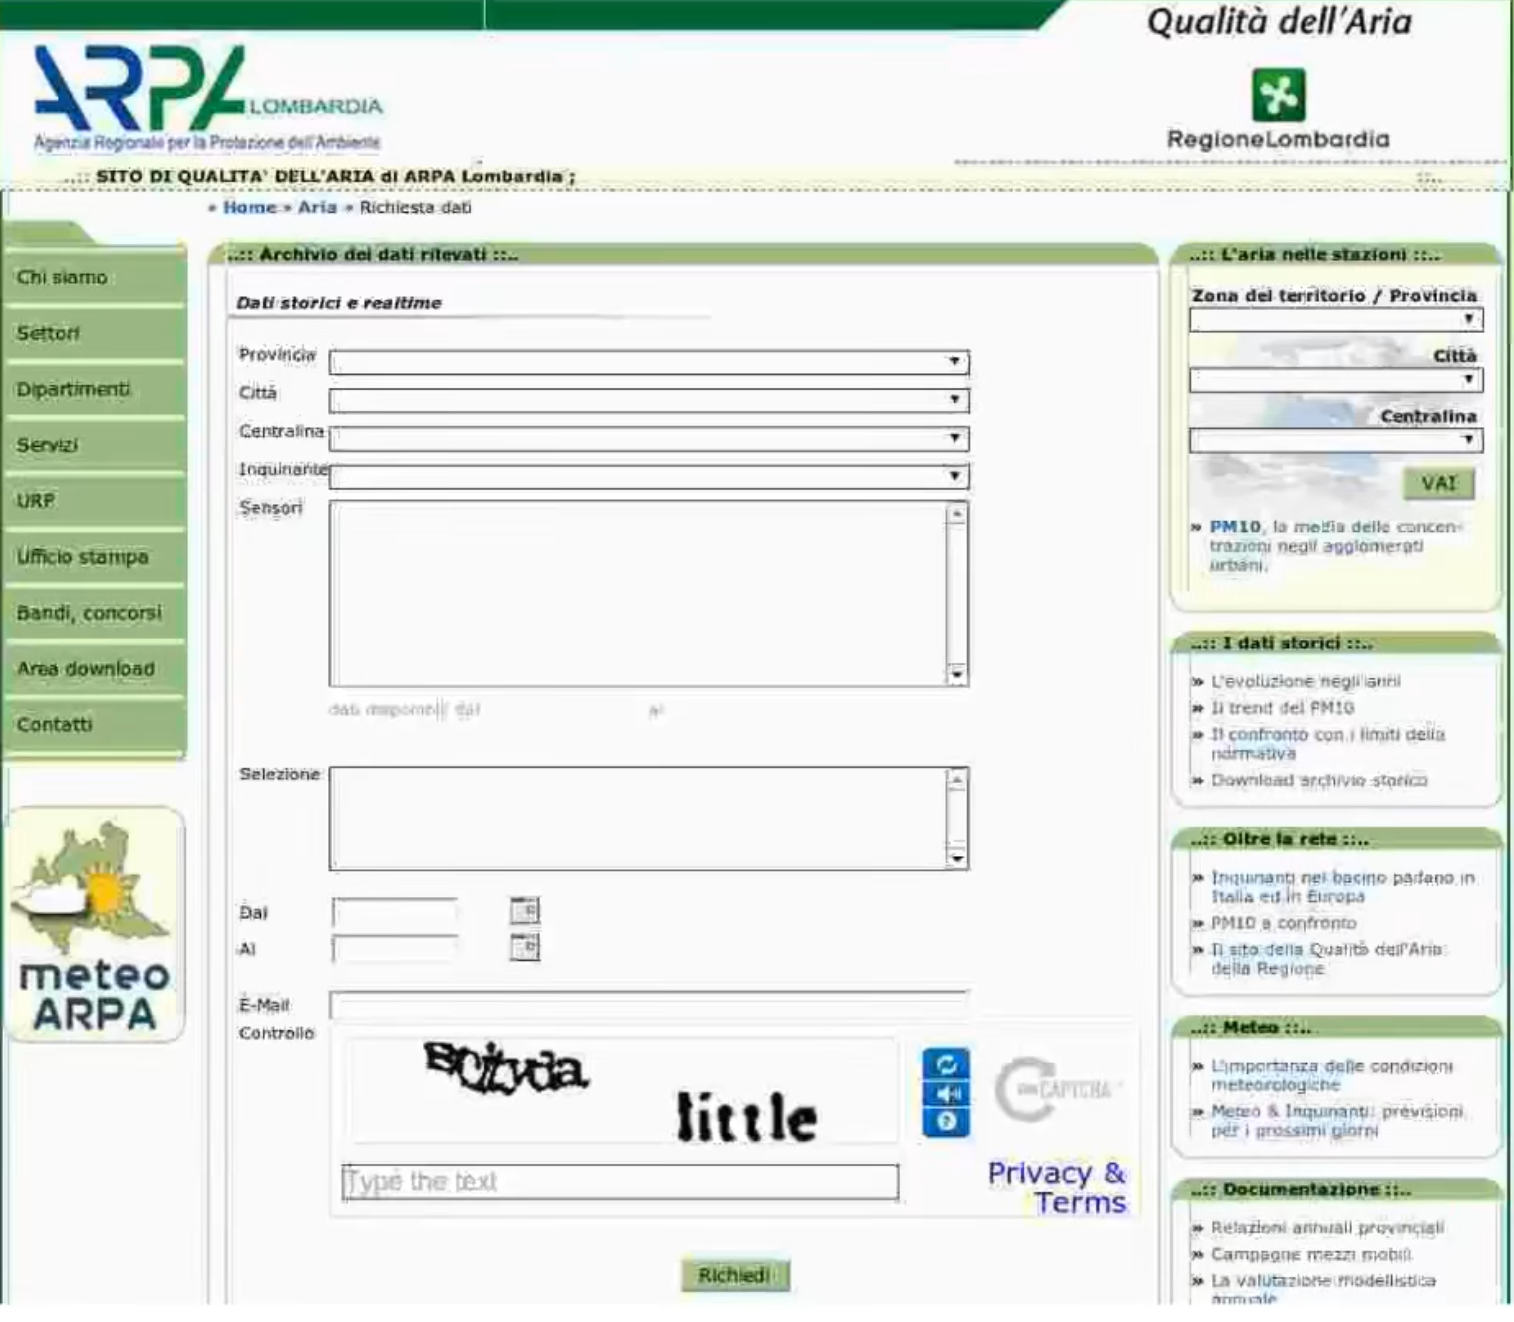
\includegraphics[width=0.7\linewidth]{img/arpa.png}\hspace*{\fill}
    \caption{Form per la richiesta di dati sul sito Arpa (fonte: Trentini)}
    \label{fig:arpa}
\end{figure}


La possibilità di \quotestyle{poter fare i conti in tasca} a enti come Arpa, 
viene spesso contrapposta al diritto alla privacy, anche in 
modo completamente ingiustificato, quando invece numerosi sarebbero i vantaggi 
del rendere accessibili più informazioni agli utenti.

A questo scopo sono state favorite varie iniziative per aumentare la quantità di 
dati liberi disponibile. 
Tra queste va ricordata nel 2009, negli Stati Uniti, la creazione del sito 
Data.gov\footnote{\url{https://www.data.gov/}}, 
con lo scopo di raccogliere in un unico portale la maggior parte dei dataset 
aperti di enti americani. 
Non passerà molto tempo prima che altri paesi si uniscano al movimento. 
L'Italia in particolare creerà nel 2011 il proprio portale 
dati.gov.it\footnote{\url{https://www.dati.gov.it/}}, mentre l'Unione Europea seguirà 
nel 2012\footnote{\url{https://data.europa.eu/euodp/it/home}}. 

\skipline
Questo lavoro è da intendere come una dimostrazione delle analisi realizzabili 
tramite dati pubblici, e di quanti altri studi sarebbe possibile eseguire se fossero 
disponibili le informazioni mancanti. 

Una delle domande che ci si potrebbe porre, è se il pavé, a Milano, 
influisca sull'incidentalità. 
Un'altra questione interessante riguarda gli autovelox, e come questi influiscano sulla 
la guida dei conducenti in loro prossimità. 
O ancora se le linee dei trasporti pubblici aumentino o diminuiscano il numero di sinistri. 

Altre questioni interessanti potrebbero essere:
\begin{itemize}
    \item Quali sono le strade più pericolose in Italia?
    \item Si ha più probabilità di essere coinvolti in un sinistro in città o su una 
    strada extraurbana? 
    \item Le linee di trasporto pubblico influenzano il traffico positivamente 
    o negativamente?
    \item Il numero di passeggeri influisce sulla probabilità di essere coinvolti 
    in un incidente? 
    \item Esistono fattori di distrazione per il conducente di un'automobile? 
\end{itemize}

%%%%%%%%%%%%%%%%%%%%%%%%%%%%%%%%%%%%%%%%%%%%%%%%%%%%%%
\chapter{Origine dei dati}

\section{Incidenti}
\todo{ATOK}

La maggior parte dei dataset utilizzati in questo lavoro 
provengono dall'Istituto nazionale di statistica, in particolare 
dall'archivio di dati non geolocalizzati su incidenti stradali in 
Italia\footnote{\url{https://www.istat.it/it/archivio/87539}}. 
Questo dataset contiene un'ampia gamma di campi, tra cui ora, 
mese, giorno della settimana in cui è avvenuto l'incidente, 
ma anche informazioni sui passeggeri, la natura del sinistro e il tipo di strada. 
Particolarmente interessanti sono anche i campi riguardanti la tipologia di incrocio 
in cui è avvenuto il sinistro, come rettilineo, rotonda o semaforo. 

\lighttext{(\\
    \indent anno, provincia, \\
    \indent comune, giorno,\\
    \indent localizzazione\_incidente\footnote{zona incidente come urbana, extraurbana 
    o autostrada}\\
    \indent tipo\_di\_strada\footnote{numero di carreggiate della strada},\\
    \indent pavimentazione,\\
    \indent intersezione\_o\_non\_interse3\footnote{tipo di intersezione},\\
    \indent segnaletica,\\
    \indent condizioni\_meteorologiche, \\
    \indent natura\_incidente,\\
    \indent tipo\_veicolo\_a\footnote{questo campo è ripetuto per altri due veicoli},\\
    \indent veicolo\_\_a\_\_\_et\_\_conducente\footnote{questo e i due campi successivi 
    sono ripetuti anche per i passeggeri},\\
    \indent veicolo\_\_a\_\_\_sesso\_conducente,\\
    \indent veicolo\_\_a\_\_\_esito\_conducente, \\
    \indent morti\_entro\_24\_ore,\\
    \indent morti\_entro\_30\_giorni\footnote{questo insieme non contiene la categoria 
    precedentemente},\\
    \indent feriti, Ora, trimestre\footnote{prima del 2014 questo campo è sostituito dall'anno}\\
)}

Per quanto riguarda i dati geolocalizzati, 
la fonte è invece il giornale online TheSubmarine 
che, in un articolo riguardante l'incidentalità a Milano \cite{SUBMARINE:1}, 
ha ottenuto dall'ente Istat la pubblicazione di una parte dei dati inerenti 
incidenti avvenuti in città, nel 2016, con la relativa 
posizione\footnote{La fonte è la stessa del dataset precedente, ma i proprietari 
dell'articolo sono riusciti a fare pubblicare da Istat una parte delle posizioni 
geolocalizzate di incidenti a Milano, normalmente private per proteggere la privacy 
delle persone coinvolte.}. 
Il dataset in questione è abbastanza scarno, contiene solamente 
l'incidente con la relativa posizione, indicata tramite coordinate geografiche. 

Infine l'ultimo dataset è stato reperito sul sito di 
ACI\footnote{Automobile Club Italia} \cite{ACI:1}. 
Questi dati, riferiti a autostrade e strade provinciali, riportano anche il 
nome della via in cui è avvenuto l'incidente, oltre a informazioni come 
l'orario, il mese o il giorno della settimana. 

\lighttext{(\\
    \indent COD REG,REGIONE,\\
    \indent COD PROV,PROVINCIA,\\
    \indent NOME STRADA: codice e nome della strada,\\
    \indent INC: numero di incidenti\footnote{Potrebbero esserci più incidenti per 
    riga, la divisione è eseguita in base alla caratteristica principale del file, 
    come ora, giorno della settimana ecc.},\\
    \indent MOR,FER,\\
    \indent NVEI: numero di veicoli coinvolti\\
)}

\section{Autovelox}
\todo{ATOK}

Una delle prime domande che ci si è posti, è stata se gli autovelox, installati 
nel tentativo di ridurre la velocità delle vetture, avessero influenza sul numero 
degli incidenti del luogo. 

Un primo dataset individuato, che riguardasse le coordinate 
degli autovelox fissi, è stata una mappa 
GoogleMyMaps\footnote{\url{https://www.google.com/maps/d/viewer?mid=1CBgMTvIDnbGo22-Y1f3rVcbeX4C0v_w1&ll=45.365557951599605\%2C10.03650113755961&z=8}} 
creata da un utente anonimo, dunque senza possibilità di verificarne l'autenticità. 
Per evitare di fare uso di informazioni non corrette, si è preferito scartare 
questa fonte. 

I dati utilizzati, invece, sono stati ottenuti tramite il sito OpenStreetMaps, 
realizzando una query per selezionare solo gli autovelox presenti a Milano. 
Per restringere il campo di ricerca alla sola città, si è fatto uso delle 
Overpass API\footnote{Application Programming Interface, cioè un insieme di 
procedure utili, in questo caso all'ottenimento di dati, ma che permettono 
lo svolgimento di svariati compiti.}\footnote{\url{https://overpass-turbo.eu/}}, 
specifiche per OpenStreetMaps, utilizzando il codice riportato nel riquadro seguente: 

\begin{code}
[out:json];
node({{bbox}})["highway"="speed_camera"];
out meta;
\end{code}

Il dataset ricavato, purtroppo, non contiene informazioni riguardanti quando gli 
autovelox siano stati installati, fattore importante per capirne l'effetto 
sul traffico e sugli incidenti. 
Tuttavia il sito web Ztlmilano 
contiene un articolo nel quale specifica una lista di 
autovelox installati nel 2014 \cite{ZTLMILANO:1}. 
Sapendo che il dataset di OpenStreetMaps è stato aggiornato fino ad oggi, 
è possibile ricavare la posizione precisa di questi ultimi. 

La lista di Ztlmilano contiene i seguenti autovelox: 

\begin{center}
    \def\arraystretch{1.5}%  
    \begin{tabular}{ |c|c| } 
    \hline
    Numero & Localizzazione dell'autovelox \\ 
    \hline
    \rowcolor{TableGray}
    1   &   Viale Monte Ceneri  dir. Lugano\\
    2   &   Viale Monte Ceneri dir. Serra\\
    \rowcolor{TableGray}
    3   &   Cavalcavia del Ghisallo\\
    4   &   Viale Serra dir. Lotto\\
    \rowcolor{TableGray}
    5   &   Viale Serra dir. Monte Ceneri\\
    6   &   Via Fermi\\
    \rowcolor{TableGray}
    7   &   Viale Fulvio Testi direz. perif.\\
    8   &   Viale Fulvio Testi direz. centro\\
    \rowcolor{TableGray}
    9   &   Viale Palmanova  direz. centro\\
    10  &   Viale Palmanova\\
    \rowcolor{TableGray}
    11  &   Via Ferrari direz. Ripamonti\\
    12  &   Via Ferrari\\
    \rowcolor{TableGray}
    13  &   Via Chiesa Rossa\\
    14  &   Via dei Missaglia direz. centro\\
    \rowcolor{TableGray}
    15  &   Via dei Missaglia direz. periferia\\
    16  &   Viale Famagosta\\
    \rowcolor{TableGray}
    17  &   Via Parri\\
    18  &   Via Parri\\
    \hline
    \end{tabular}
    \label{ztl-milano}
\end{center}

Il campi della tabella ripetuti sono dovuti al fatto che alcuni autovelox sono stati 
installati in entrambe le direzioni. 

\section{Patentati}
\todo{ATOK}

Un'importante necessità in un'indagine di questo tipo, è avere un contesto in cui inserire 
i risultati ottenuti. 
Senza conoscere il numero di vetture che transitano quotidianamente sulle strade oggetto 
di analisi, non è possibile capire il peso degli incidenti che lì vi avvengono.

Si è dunque tentata una ricerca, infruttuosa, di dataset sul traffico stradale nel periodo 
dal 2010 al 2018. 
Queste informazioni si sono cercate, per la zona di Milano, nei principali 
siti di open data, con parole chiave come \quotestyle{traffico milano} e 
\quotestyle{flussi autostrade}. 
Si è inoltre controllato sul sito di Autostrade per 
l'Italia\footnote{\url{http://www.autostrade.it/it/home}}, 
ma le uniche informazioni trovate sono in tempo reale. 

Non avendo trovato alcun dato sull'argomento, si è tentato di realizzare 
alcune stime del numero di automobili circolanti per regione, e a Milano. 

I dati sui patentati per regione, che sono stati utilizzati per stimare il traffico 
regionale, proviene dal sito del Ministero delle Infrastrutture e 
Trasporti\footnote{\url{http://dati.mit.gov.it/catalog/dataset/patenti}}. 


\lighttext{(\\
    \indent id: progressivo numerico,\\
    \indent provincia\_residenza, \\
    \indent categoria\_patente: più elevata, \\
    \indent abilitato\_a: abilitazioni A2-A4 della patente, \\
    \indent data\_rilascio, \\
    \indent nazionalita: di emissione \\
)}


Questo dataset è formato da un'ampia quantità di informazioni, 
non utili al fine dell'analisi, 
si è preferito quindi usare una sintesi di queste, proveniente da 
un'infografica che riassume i dati in questione \cite{INFOGRAFICA_MIT:1}. 
In particolare, da questo file si è utilizzato solamente 
il numero di patentati per regione. 

\`E anche necessario chiedersi quanto, il numero delle persone che hanno ottenuto 
una patente per regione, sia un fattore valido con cui stimare il traffico, 
tenendo conto del fatto che molti individui non vivono nella zona 
in cui hanno ottenuto la patente, e altre potrebbero spostarsi ogni giorno in altri 
luoghi per questioni di lavoro. 
\`E ragionevole, pertanto, supporre che tale stima non sarà mai tra le più accurate, 
e in caso di grandi disparità tra regioni, si potrebbe dover invalidare 
i calcoli eseguiti. 

\section{Area C di Milano}
\todo{ATOK}

Per lo stesso motivo del capitolo precedente, cioè realizzare una stima approssimativa 
del traffico, si sono cercate informazioni sugli accessi all'area C di Milano, 
in base all'orario. 

Il dataset riguardante gli accessi è stato trovato sul portale di open data 
del comune di 
Milano\footnote{\url{https://dati.comune.milano.it/organization/comunedimilano?q=area+c&sort=score+desc\%2C+metadata_modified+desc}}, 
dove sono disponibili varie tipologie di file distinti per orario, 
mese o località. 
Tra questi si è utilizzata la tipologia contenente orari e data dell'accesso. 

\lighttext{(\\
    \indent year: anno dell'accesso in area C,\\
    \indent month: mese dell'accesso in area C,\\
    \indent day: giorno dell'accesso in area C,\\
    \indent hour: ora dell'accesso in area C,\\
    \indent totale: numero di accessi nella riga,\\
    \indent areac\footnote{booleano che indica se l'area C sia attiva o meno}\\
)}

Oltre ai dati riferiti agli accessi all'area C, si è fatto uso anche di una mappa 
dei varchi di entrata e dei limiti del centro storico, 
proveniente dal sito del comune di 
Milano\footnote{\url{https://www.comune.milano.it/aree-tematiche/mobilita/area-c}}. 

Per quanto anche questa stima non sia tra le più accurate, ci si può aspettare che 
il numero di accessi corrisponda, almeno in parte, al volume di traffico di Milano. 

\section{Le zone di Milano}
\todo{ATOK}

I dataset delle zone di Milano provengono dal portale di dati geolocalizzati della 
città\footnote{\url{https://geoportale.comune.milano.it/}}, 
e contengono i poligoni che costituiscono i municipi, 
oltre a informazioni sulla superficie e il perimetro delle aree. 

\lighttext{(\\
    \indent MUNICIPIO: id della zona,\\
    \indent AREA: della zona,\\
    \indent PERIMETRO: della zona,\\
    \indent geometry\footnote{insieme di punti che formano i poligoni rappresentati nel file}\\
)}

Queste informazioni sono utili a determinare, a grandi linee, quali sono le zone 
con più incidenti a Milano. 
Il risultato ottenuto non potrà, purtroppo, essere dei più precisi data l'ampiezza 
delle sezioni, ma anche il fatto che le zone non fotografano solo le superfici stradali, 
ma anche abitazioni e terreni, dove naturalmente non avvengono incidenti. 

Pertanto, il numero di sinistri per zona così ricavato, 
è da considerarsi come un'approssimazione per difetto, o una stima del 
\quotestyle{lower bound}, perché il valore è abbassato dalle aree in cui non 
possono avvenire incidenti tra vetture. 
Viceversa, i calcoli che utilizzano solamente la superficie stradale avranno 
inevitabilmente valori maggiori. 

\section{Il meteo}
\todo{ATOK}

Per quanto riguarda i dati sul meteo, si è tentato di utilizzare le informazioni 
provenienti dalle centraline Arpa. 
Dopo un veloce controllo delle loro posizioni, visibili in figura \ref{fig:centraline-arpa}, 
si è notato che il dataset non contiene tutte le stazioni di Milano. 

\begin{figure}
    \hfill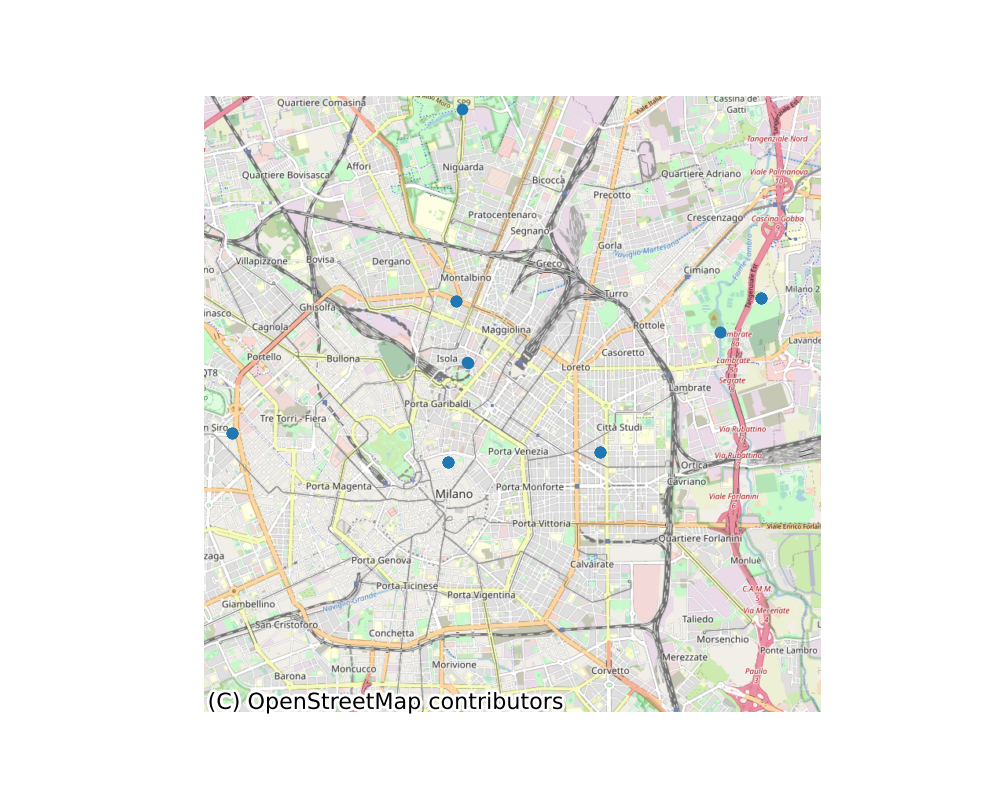
\includegraphics[width=0.7\linewidth]{../src/meteo/centraline_arpa.png}\hspace*{\fill}
    \caption{Centraline Arpa a Milano}
    \label{fig:centraline-arpa}
\end{figure}

Per esempio, utilizzando una lista di centraline meteo completa, come quella su 
Centrometeolombardo\footnote{\url{http://www.centrometeolombardo.com/content.asp?CatId=272&ContentType=Stazioni}}, 
si nota che mancano quelle di Abbiategrasso Sud e Cadorna. 
Inoltre, per mancanza di dati precisi sul giorno degli incidenti, 
è superfluo avere informazioni con posizione e data così precise. 

Si è dunque optato per un dataset trovato sul sito 
Zenodo\footnote{\url{https://zenodo.org/record/3992354}},
contenente temperature, umidità, e velocità del vento, 
misurati ogni ora a Milano, a partire dal 2008, fino al 2018. 

\lighttext{(\\
    \indent Date\_Time: contiene giorno, mese e anno,\\
    \indent Temperature: in gradi Celsius,\\
    \indent Dew\_Point: temperatura di condensazione,\\
    \indent Humidity: umidità,\\
    \indent Wind\_Speed: velocità del vento\\
)}

\section{Trasporti pubblici}
\todo{ATOK}

Un altro fattore di cui ci si è chiesti l'influenza sull'incidentalità, è la 
presenza, nella via o viale, di trasporti pubblici. 

I dati riguardanti questi ultimi, provengono da due fonti, i primi sono 
dati riferiti alle linee ATM, scaricati sul sito del comune di 
Milano\footnote{\url{https://dati.comune.milano.it/dataset/ds532-atm-composizione-percorsi-linee-di-superficie-urbane}}, 
contenenti informazioni quali il numero identificativo della linea, 
la lunghezza e il tipo di mezzo. 

\lighttext{(\\
    \indent linea: numero della linea,\\
    \indent mezzo: bus, filobus o tram,\\
    \indent percorso: identificatore del percorso,\\
    \indent verso, nome,\\
    \indent tipo\_perc: Canonico o Barrato,\\
    \indent lung\_km, num\_ferm,\\
    \indent geometry\footnote{insieme di linee che formano i percorsi contenuti nel file}\\
)}

Dallo stesso sito proviene anche il file riguardante gli autobus turistici, che 
contiene, in particolare, solo le aree di 
sosta\footnote{\url{https://dati.comune.milano.it/dataset/ds740_sosta_bus_gt_turistici}}. 

Si è anche fatto uso di un dataset contenente 
solamente le linee tranviarie, reperito dal portale di dati geolocalizzati 
del comune di 
Milano\footnote{\url{https://geoportale.comune.milano.it/ATOM/SIT/DBT2012/DBT2012_STRATO_01_Dataset_1.xml}}. 
Questo documento è molto ampio e contiene altri livelli di informazioni, tra cui 
le strade, le ferrovie o le piste ciclabili passanti per la città. 

La principale funzione di questi dataset è l'ottenere i percorsi delle linee di trasporto pubblico, 
per confrontare il numero di incidenti, nelle vie in cui viaggiano autobus, rispetto a 
quelle in cui sono presenti solo autovetture private. 

\section{Autostrade e manto stradale}
\todo{ATOK}

Puramente per la realizzazione di alcune mappe, quindi non a scopo di analisi 
ma più di visualizzazione, si è tentata la ricerca di dati geolocalizzati sulle 
strade Italiane. 

Il primo dataset individuato, riguardante il manto  stradale, è stato trovato sul sito 
internet dell'ente  
ANAS\footnote{\url{http://dati.mit.gov.it/catalog/dataset/grafo-stradale-anas}}. 
Tuttavia, questo consisteva in un file molto grande, contenente tutte le principali 
strade in Italia, dalla precisione superflua per le mappe che si vuole ottenere. 

Si è dunque tentato di utilizzare il dataset presente sul portale di dati geolocalizzati 
del comune di Milano\footnote{\url{https://geoportale.comune.milano.it/}}. 
Anche quest'ultimo risulta però troppo dettagliato, in quanto riporta la 
totalità del manto stradale della città. 

Come ultima risorsa, si è deciso di tracciare alcune mappe in formato 
\engstyle{geojson}\footnote{Formato di file derivato da \engstyle{Json} 
(JavaScript Object Notation), che è usato spesso per il salvataggio di informazioni, ma 
in aggiunta permette di memorizzare insiemi di punti, sotto forma di linee o poligoni, 
tramite l'apposito campo \columnstyle{geometry}.} utilizzando il sito 
Geojson.io\footnote{\url{https://geojson.io/}}, in particolare nella zona di Milano, 
per le principali autostrade, tangenziali e strade statali. 
Allo stesso modo, Geojson.io è stato utile a tracciare alcune aree in centro a Milano, 
per confrontare gli incidenti su pavé agli incidenti su asfalto. 

\section{Il turismo}
\todo{ATOK}

Durante le analisi degli incidenti autostradali, è sorto il dubbio che 
nelle annate più recenti, tra 2015 e 2018, 
fosse presente un incremento di persone in ferie in località di montagna. 
Le informazioni riguardanti il turismo, sono state utili a visualizzare questa tendenza 
tramite un campione di dati diverso. 

I dataset sul turismo in Italia, sono stati trovati nell'archivio Istat sul 
tema\footnote{\url{https://www.istat.it/it/archivio/16777}}. 
Il file originale era in formato \engstyle{xls}\footnote{Formato di memorizzazione dei file 
utilizzato spesso da Microsoft Excel}, 
contenente informazioni a partire dal 1995 
fino al 2019, sia regione per regione, sia divise tra nord, centro e sud. 
A loro volta, i documenti sono divisi in più tabelle, ognuna raffigurante un particolare 
indicatore, come produttività del lavoro, turismo nei mesi non estivi, 
tasso di turisticità\footnote{Il tasso di turisticità misura il livello di "affollamento" 
turistico in un determinato periodo (anno o mese) indicando il numero di turisti presenti 
ogni 100.000 abitanti. \cite{ONTIT:1}} 
e valore aggiunto del turismo. 

Per controllare la tendenza, sono stati necessari i dati divisi regione per regione, 
a partire dal 2010 fino al 2018, convertiti in formato csv, e sono stati scelti gli 
indicatori di turismo nei mesi non estivi, e tasso di turisticità. 

\section{Immagini del traffico}
\todo{ATOK}

Le immagini raffiguranti il traffico in tempo reale sono prese da Google 
Maps\footnote{\url{https://www.google.com/maps/}}. 

In primo luogo, si è tentato di realizzare degli screenshot direttamente dal sito, 
tuttavia le figure prese in questo modo, contengono molti punti di interesse e altri simboli, 
che coprono informazioni importanti, come i nomi delle strade. 

Per rimuovere i simboli superflui, si è fatto uso delle API di Google Maps, 
tramite il sito Jsfiddle\footnote{\url{https://jsfiddle.net/}}, un sito web che permette di 
scrivere e eseguire codice JavaScript. 

Gli screenshot realizzati rappresentano le zone nelle vicinanze dei Navigli 
e dell'incrocio tra viale Bianca Maria e viale Ventidue Marzo a Milano. 

%%%%%%%%%%%%%%%%%%%%%%%%%%%%%%%%%%%%%%%%%%%%%%%%%%%%%%
\section{Dati mancanti}

\subsection{Il pavé}
\todo{ATOK}

Nonostante le ricerche nei principali siti di 
opendata\footnote{
    \url{https://dati.comune.milano.it/dataset}, 
    \url{https://www.dati.lombardia.it/},
    \url{https://www.dati.gov.it/}}
non sembra esistere un dataset contenente informazioni sulla composizione del 
manto stradale di Milano. 
In particolare, si sono cercate le informazioni tramite parole chiave come 
\quotestyle{strada}, \quotestyle{manto stradale}, \quotestyle{pavé}, 
\quotestyle{composizione strada}. 

Una risorsa reperita durante le ricerche, è una mappa utilizzata in un articolo del blog online 
Urbanfile \cite{URBANFILE:1}. 
Dopo una rapida consultazione con l'autore tuttavia, non risulta esserci alcun 
dataset contenente informazioni riguardanti il pavé a Milano, infatti la cartina è 
stata realizzata per conoscenza personale. 

I dati che potrebbero avvicinarsi di più alle informazioni ricercate, 
sono quelli riguardanti i percorsi delle linee tranviarie. 
Basandosi su queste informazioni, e supponendo che la maggior parte delle linee dei 
tram a Milano siano in pavé, è possibile ottenere un dataset di taglia discreta. 

Tuttavia, confrontando le linee tranviarie, con la mappa di Urbanfile, 
per quanto alcune zone coincidano, non si è trovata 
somiglianza sufficiente per giustificare l'utilizzo. 

A conclusione, si è optato per tracciare una mappa utilizzando 
Geojson.io\footnote{\url{https://geojson.io/}}, come già fatto per le autostrade a Milano, 
basandosi sulla cartina trovata su Urbanfile. 

\subsection{Traffico stradale}
\todo{ATOK}

Per quanto riguarda i dati sul traffico stradale, anche in questo caso non è stato trovato un 
dataset, sia nei siti di cui si è parlato in precedenza, sia su quello di 
autostrade\footnote{\url{http://www.autostrade.it/it/home}}. 

Il primo tentativo, per avere una stima del traffico è stato la realizzazione di uno 
script per fare scraping da Google Maps. 
Questo sito infatti mostra sia il traffico in tempo reale, sia 
il traffico stimato a una determinata ora. 
Tuttavia, leggendo la documentazione, si è scoperto che non è possibile ottenere 
dati sul traffico abituale, per la mancanza delle API corrispondenti. 
D'altra parte, il traffico in tempo reale è disponibile, ma non è particolarmente utile 
poiché questo studio è stato svolto in concomitanza a un lungo periodo di quarantena 
dovuto al Covid-19, le cui limitazioni hanno ridotto in maniera significativa 
i volumi di traffico. 
Per quanto fosse stato possibile realizzare comunque uno script per effettuare 
scraping della quantità di traffico nelle strade, registrando il colore delle 
direttrici per ogni orario della giornata nei periodi interessati, si è 
optato per la ricerca di un altro dataset. 

Si è deciso, dunque, di utilizzare i dati riguardanti gli ingressi in area C, 
trovati sul sito del comune di Milano\footnote{\url{https://dati.comune.milano.it/dataset}}, 
nonostante questi non permettano una stima perfetta. 

Un altro dataset utilizzato per stimare il numero di vetture, è quello contenente 
il numero di patentati per regione, trovato nel sito del Ministero dei 
Trasporti\footnote{\url{dati.mit.gov.it/catalog/dataset/patenti}}. 
I dati, disponibili fino al 2019, sono divisi in file per regione e 
contengono anche informazioni riguardanti la provincia e data di conseguimento della 
patente, oltre al tipo di certificato ottenuto. 

\subsection{Dati su strade, incroci, semafori}
\todo{ATOK}

In alcuni capitoli, in particolare quelli riguardanti le tipologie di incidente e 
di incrocio, i dati disponibili non permettono di realizzare delle stime sulle 
percentuali di strade per le diverse categorie. 
In altre parole, non si ha modo di sapere, in un'area come Milano, quanti incroci 
per esempio siano con semaforo, o della categoria rotonda, 
rispetto al numero totale di intersezioni. 

Per stimare queste percentuali si sono cercati, innanzitutto, articoli o dataset online, con 
parole chiave come \quotestyle{numero semafori Milano} o \quotestyle{strade incroci semafori}. 
Non trovando alcun riscontro, si è ricercato l'argomento nei principali siti contenenti 
dataset, di cui si è parlato in precedenza. 

Le informazioni più simili a ciò che si stava cercando, 
sono state trovate sul portale di dati geolocalizzati 
del comune di Milano, nei dataset contenenti i tratti stradali. 
Questa collezione contiene vari livelli di informazioni, tra cui 
\columnstyle{Area di circolazione veicolare}, 
\columnstyle{Area di circolazione pedonale} e \columnstyle{Area di circolazione ciclabile}, 
tuttavia, in nessuno di questi layer, si sono trovate risorse utili a dividere, 
per esempio, intersezioni segnalate da incroci con semaforo. 

Inoltre, per la maggior parte dei livelli, non sono state reperite informazioni 
sul significato delle colonne presenti nei dataset come \columnstyle{GZ\_STR\_TY} o 
\columnstyle{GZ\_STR\_TYF}\footnote{Il dataset trovato aderisce al regolamento UE n. 1089/2010, 
tuttavia, leggendo questo documento, non è stato possibile reperire informazioni sulle colonne 
in questione \cite{REGOLAMENTOUE:1}}. 

Le ricerche di un file contenente indicazioni su questi metadati sono state eseguite sia 
sul sito del comune di Milano sia, in generale, tramite motore di ricerca, con parole chiave 
come \quotestyle{ID\_ZRIL milano} o \quotestyle{ID\_ZRIL metadati}. 
Nel caso di quest'ultimo, si è ipotizzato, tracciando una parte dei valori della colonna, 
che fosse un identificatore univoco del territorio, ipotesi confermata 
da un pdf trovato sul sito 
Cittametropolitana\footnote{\url{https://www.cittametropolitana.mi.it/export/sites/default/DeCiMetro/DOCUMENTI-DA-SCARICARE/Manuale-civici.pdf}}. 

%%%%%%%%%%%%%%%%%%%%%%%%%%%%%%%%%%%%%%%%%%%%%%%%%%%%%%
%\clearpage
\chapter{Analisi sull'incidentalità}

Per quanto riguarda i dati sugli incidenti avvenuti in Italia, 
sono disponibili due dataset molto ampi. 
Il primo, rilasciato da Istat, contiene campi quali data, ora, 
numero di persone a bordo, tipo di incrocio e tipo di veicolo. 
Queste informazioni sono presenti a partire dal 2010 fino al 2018. 
Il secondo è invece messo a disposizione da Automobile Club D'Italia (ACI) 
e contiene dati simili, 
aggiungendo il luogo dell'incidente, su autostrada o strada provinciale, 
inteso come il nome della strada, il che permette di avere una minima localizzazione del 
sinistro. 

%%%%%%%%%%%%%%%%%%%%%%%%%%%%%%%%%%%%%%%%%%%%%%%%%%%%%%
\section{Dati Geolocalizzati}

\subsection{Incidenti}
\todo{ATOK}

I dati riguardanti gli incidenti geolocalizzati sono disponibili in un dataset 
contenente una lista di punti indicanti latitudine e longitudine dell'evento. 
Ciò che delude, è che non è presente nessuna informazione aggiuntiva, 
oltre alla posizione. 

Controllando la distribuzione degli incidenti, 
si nota, dalla mappa destra nella figura \ref{fig:heatmap-municipi} come questi, 
a Milano abbiano concentrazioni più alte, 
in alcuni punti di interesse della città, come Piazzale Loreto, le circonvallazioni 
interna e esterna\footnote{Si evidenzieranno, in particolare, Corso Ventidue Marzo 
e la zona dei Navigli}, Piazza Kennedy e Cavalcavia del Ghisallo. 

Questa figura è stata realizzata approssimando ogni coordinata di incidente, che  
normalmente ha precisione a sette cifre decimali, a cinque numeri dopo la virgola. 
Contando i punti uguali, è stato possibile aggregare sinistri che avvengono in zone 
vicine. 
Questi dati elaborati sono poi stati memorizzati nel file reperibile al 
percorso:\\ 
\filenamestyle{dataset/incidenti/incidenti\_round.csv} 

Sarebbe interessante sapere se esistano zone con maggiore concentrazione 
di incidenti rispetto alla media, e ottenere un indice numerico 
della pericolosità di una determinata zona. 

Nella mappa sinistra della figura \ref{fig:heatmap-municipi}, si è divisa 
la città di Milano in base ai diversi municipi, ed è possibile 
osservare che nel centro storico si ha la più alta concentrazione di sinistri. 

\begin{figure}
    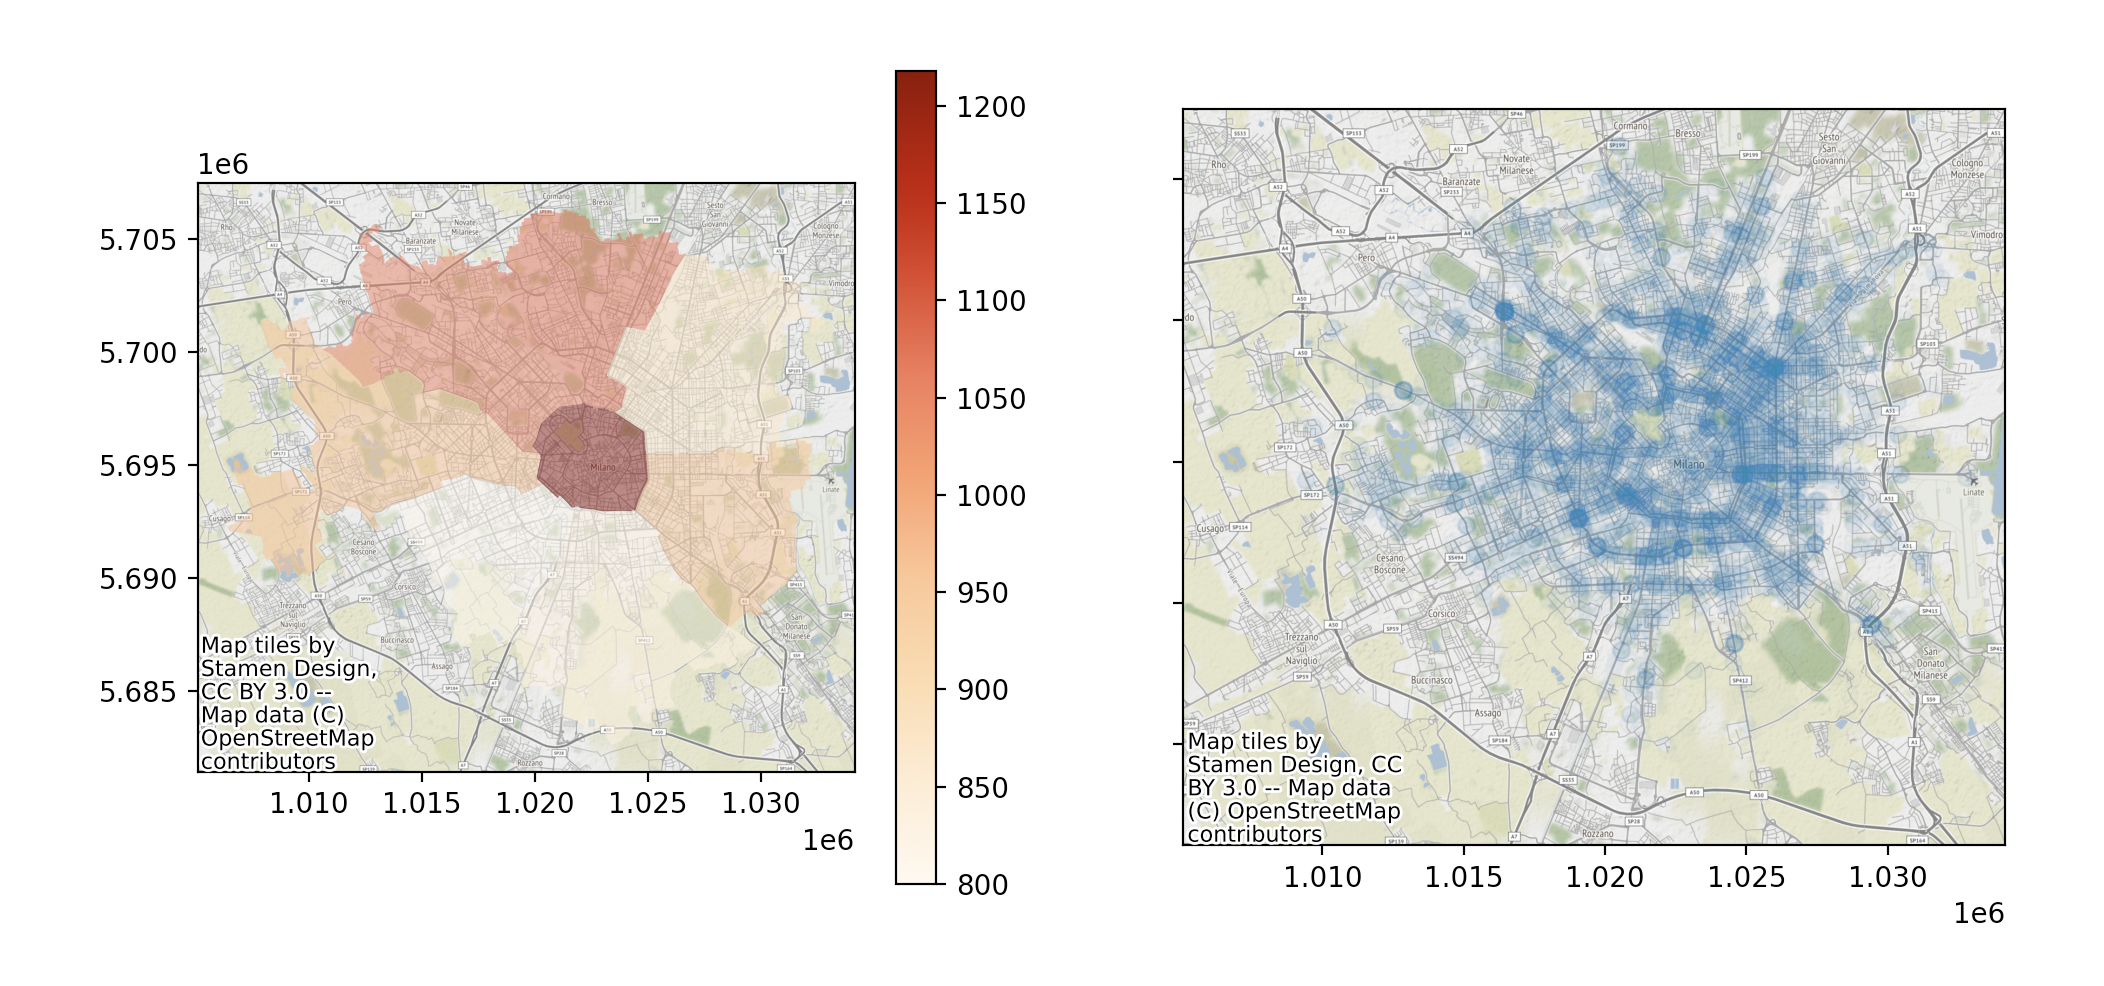
\includegraphics[width=\linewidth]{../src/municipi_milano/incidenti_municipio.png}
    \caption{Incidenti a Milano per municipio}
    \label{fig:heatmap-municipi}
\end{figure}

Non tutte le zone hanno la stessa superficie, e ovviamente sezioni più ampie hanno un maggior 
numero di strade. Avendo a disposizione l'area dei vari municipi, 
è possibile calcolare la media di incidenti al chilometro quadrato per zona. 
I risultati sono riportati negli istogrammi sottostanti. 

\begin{code}    
inc = gp.GeoSeries(df).sort_index()

area = pd.Series(data['AREA'], index=data['MUNICIPIO'])
incidenti = pd.Series(inc, index=inc.index)

# trasformazione in chilometri quadri
incidenti_per_zona = (incidenti / area) * 1000000 
\end{code}

\begin{figure}
    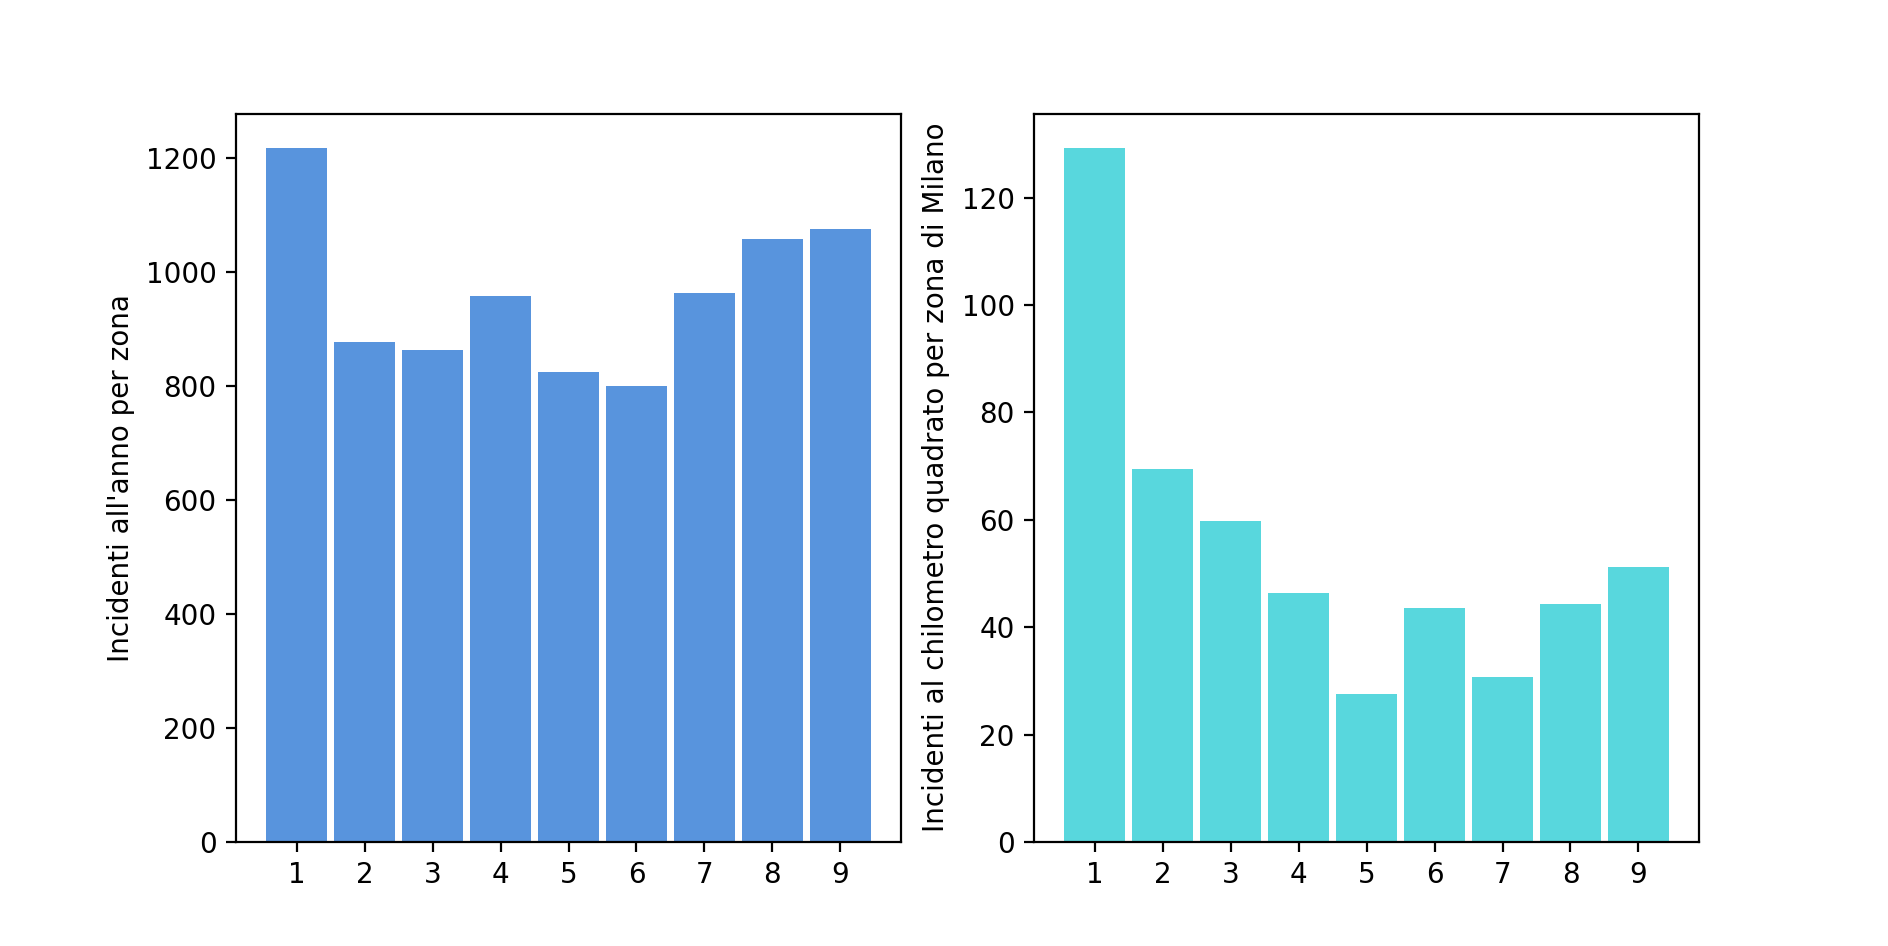
\includegraphics[width=\linewidth]{../src/municipi_milano/incidenti_superf.png}
    \caption{Incidenti a Milano per zona e in base alla superficie della zona}
    \label{fig:incidenti-chilometro}
\end{figure}

Nella figura \ref{fig:incidenti-chilometro} spicca, sia nel grafico di sinistra, rappresentante 
il numero di incidenti totali per zona, che in 
quello di destra, che contiene il volume di sinistri divisi per l'area del municipio, 
la zona 1, cioè quella del centro storico. 
La causa dell'alta quantità di eventi può essere ricondotta alla superficie minore 
di questa area rispetto agli altri municipi. 

Una volta creata la tendenza generale di ogni zona, è possibile confrontare i risultati 
ottenuti con il numero di incidenti in aree più ristrette come, per esempio, 
attorno a piazzale Loreto. 

\begin{figure}
    \hfill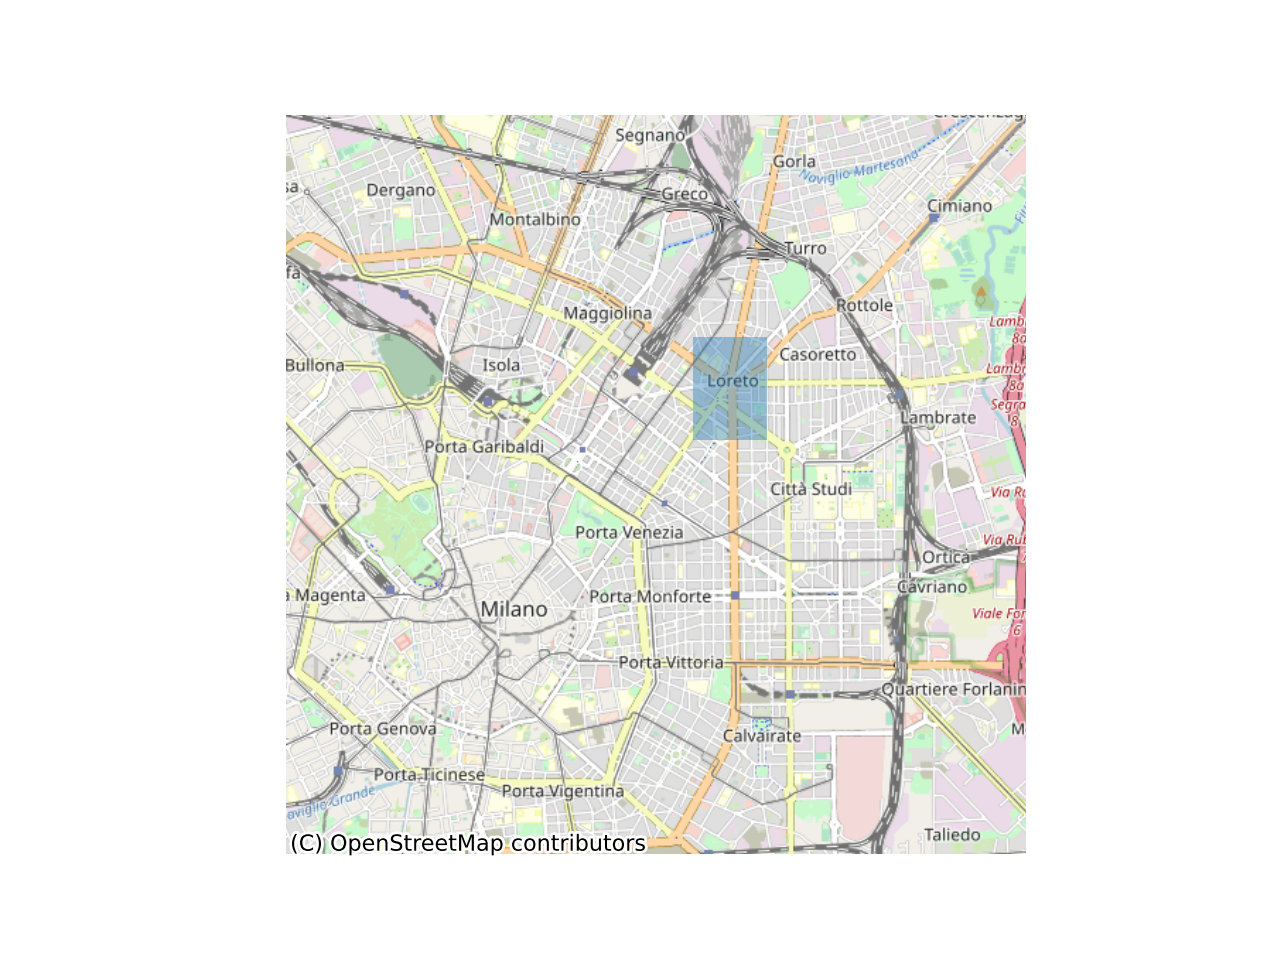
\includegraphics[width=0.7\linewidth]{../src/municipi_milano/zona_loreto.png}\hspace*{\fill}
    \caption{Zona presa in considerazione per piazzale Loreto}
    \label{fig:zona-loreto}
\end{figure}

\begin{code}
loreto = geometry.Polygon([p1, p2, p4, p3])

loreto_incidenti = 0
for point in incidenti['geometry']: 
    point = geometry.Point(point)

    if loreto.contains(point): 
        loreto_incidenti += 1

area_loreto = loreto.area * data['AREA'].iloc[0] / geometry.Polygon(data['geometry'].iloc[0]).area
area_loreto_inc = loreto_incidenti * 1000000 / area_loreto
\end{code}

Il numero di incidenti per chilometro che risultano, nell'area considerata in figura 
\ref{fig:zona-loreto}, sono $231.06$. 
Considerando che la zona con massimo valore ottenuto è il centro storico, 
con circa $120$ incidenti per chilometro quadrato, è possibile affermare 
che Piazzale Loreto sia una zona ad alta incidentalità. 

Va anche tenuto in considerazione che, come spiegato nel capitolo sull'origine dei dati, 
prendendo una qualsiasi area di strade, si avrà un numero di sinistri per chilometro quadrato 
molto maggiore rispetto a quello delle aree municipali, per la presenza di zone dove  
le automobili non possono viaggiare, come gli edifici e parchi. 

Sorge spontaneo domandarsi perché il centro storico risulti tra le aree con maggiore 
incidentalità, il volume di traffico, e quindi di incidenti, non dovrebbe essere abbassato 
della presenza dell'area C?

\begin{figure}
    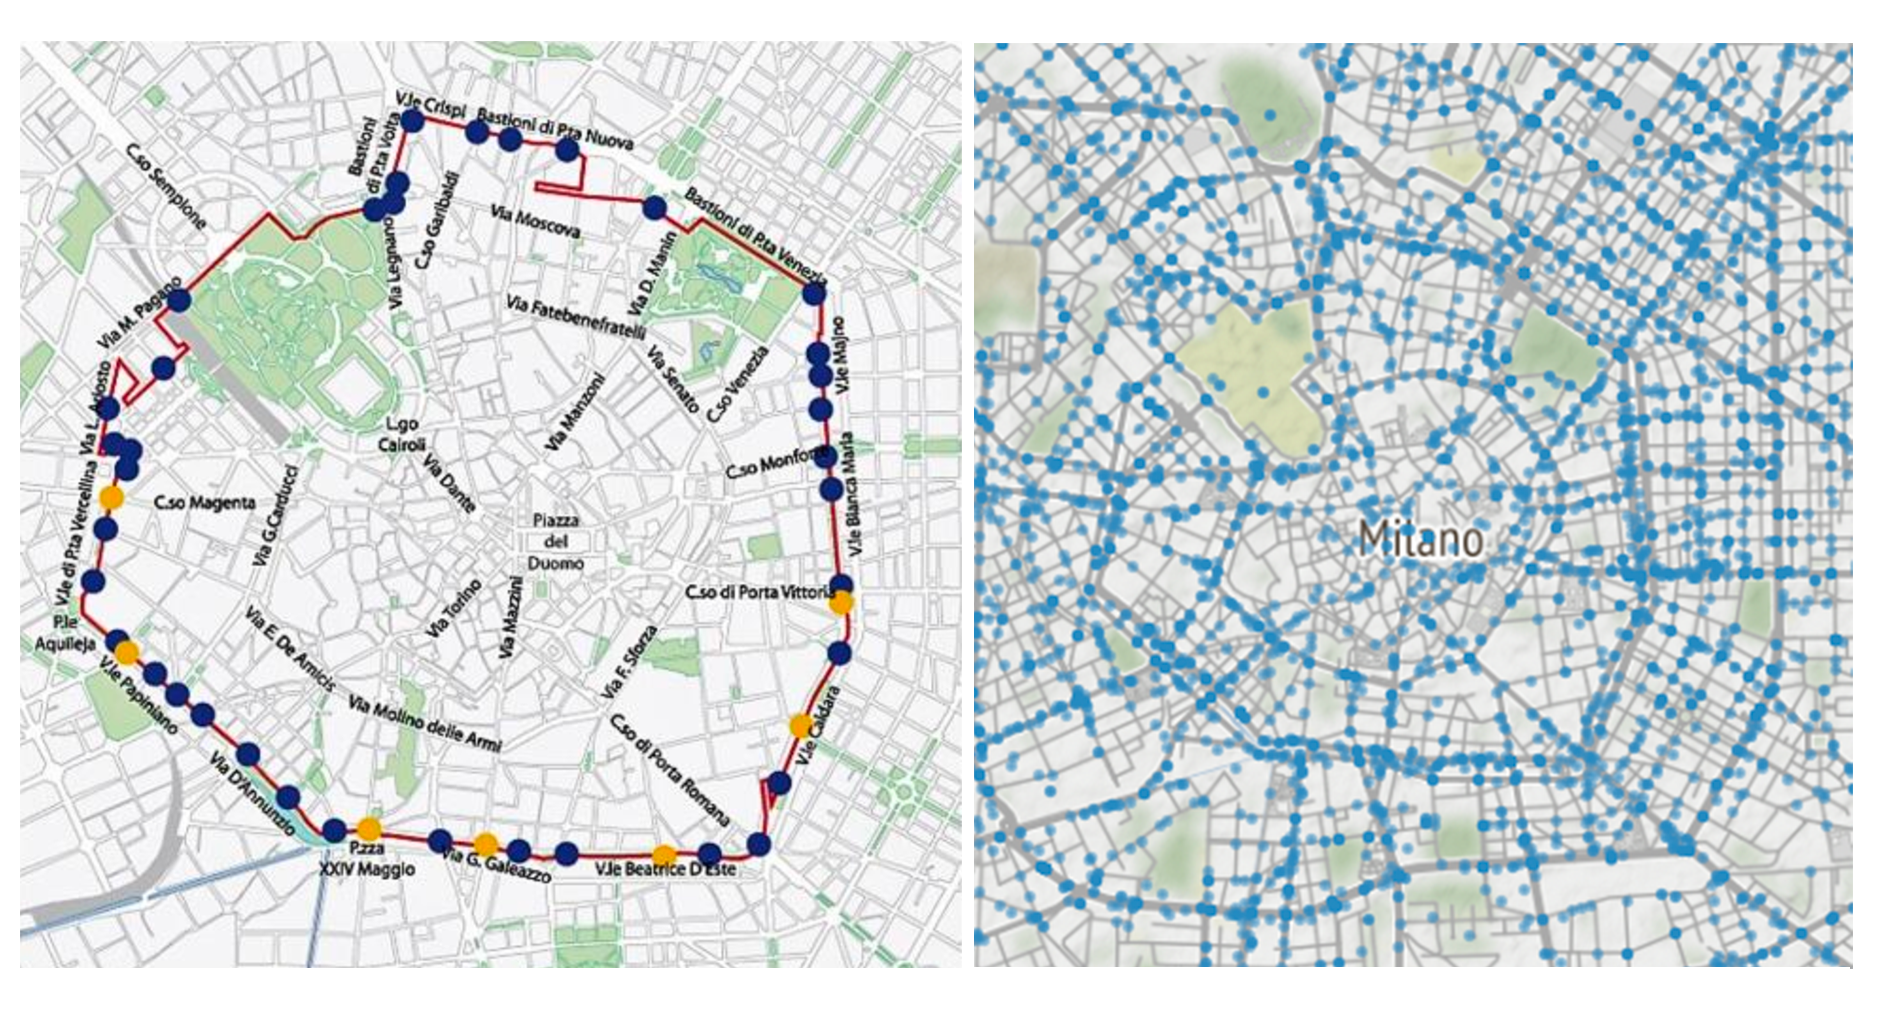
\includegraphics[width=\linewidth]{../src/area_c/area_c_incidenti.png}
    \caption{Perimetro dell'area C e incidenti nella stessa zona}
    \label{fig:perimetro-area-c}
\end{figure}

Dopo più attenta osservazione del perimetro della zona a traffico limitato, 
visibile nell'immagine a sinistra nella 
figura \ref{fig:perimetro-area-c}, è possibile precisare che la maggior parte degli 
incidenti avvengono sulla circonvallazione interna, 
situata fuori dall'area C, ma compresa nel centro storico di Milano. 

Prendendo in considerazione solamente l'area C, il numero di incidenti scende a $46.83$ 
per chilometro quadrato, di gran lunga minore rispetto al valore del centro storico. 
\`E corretto, pertanto, concludere che la riduzione del traffico veicolare, per effetto 
dell'area C, ha impatto considerevole sull'incidentalità. 

%\clearpage
\subsection{Incidenti e Linee dei Trasporti Pubblici}
\todo{ATOK}

Proseguendo con la serie di questioni poste nell'introduzione, ci si è chiesti quale 
fosse l'effetto delle linee di trasporti pubblici, come tram e autobus, 
sull'incidentalità a Milano. 

Il dataset dei tragitti dei trasporti pubblici copre una superficie più ampia rispetto a 
quello degli incidenti, dopo aver eliminato alcune linee di autobus che risultavano 
troppo in periferia, si ottiene la mappa sinistra nella figura \ref{fig:geo-trasporti}: 

\begin{figure}
    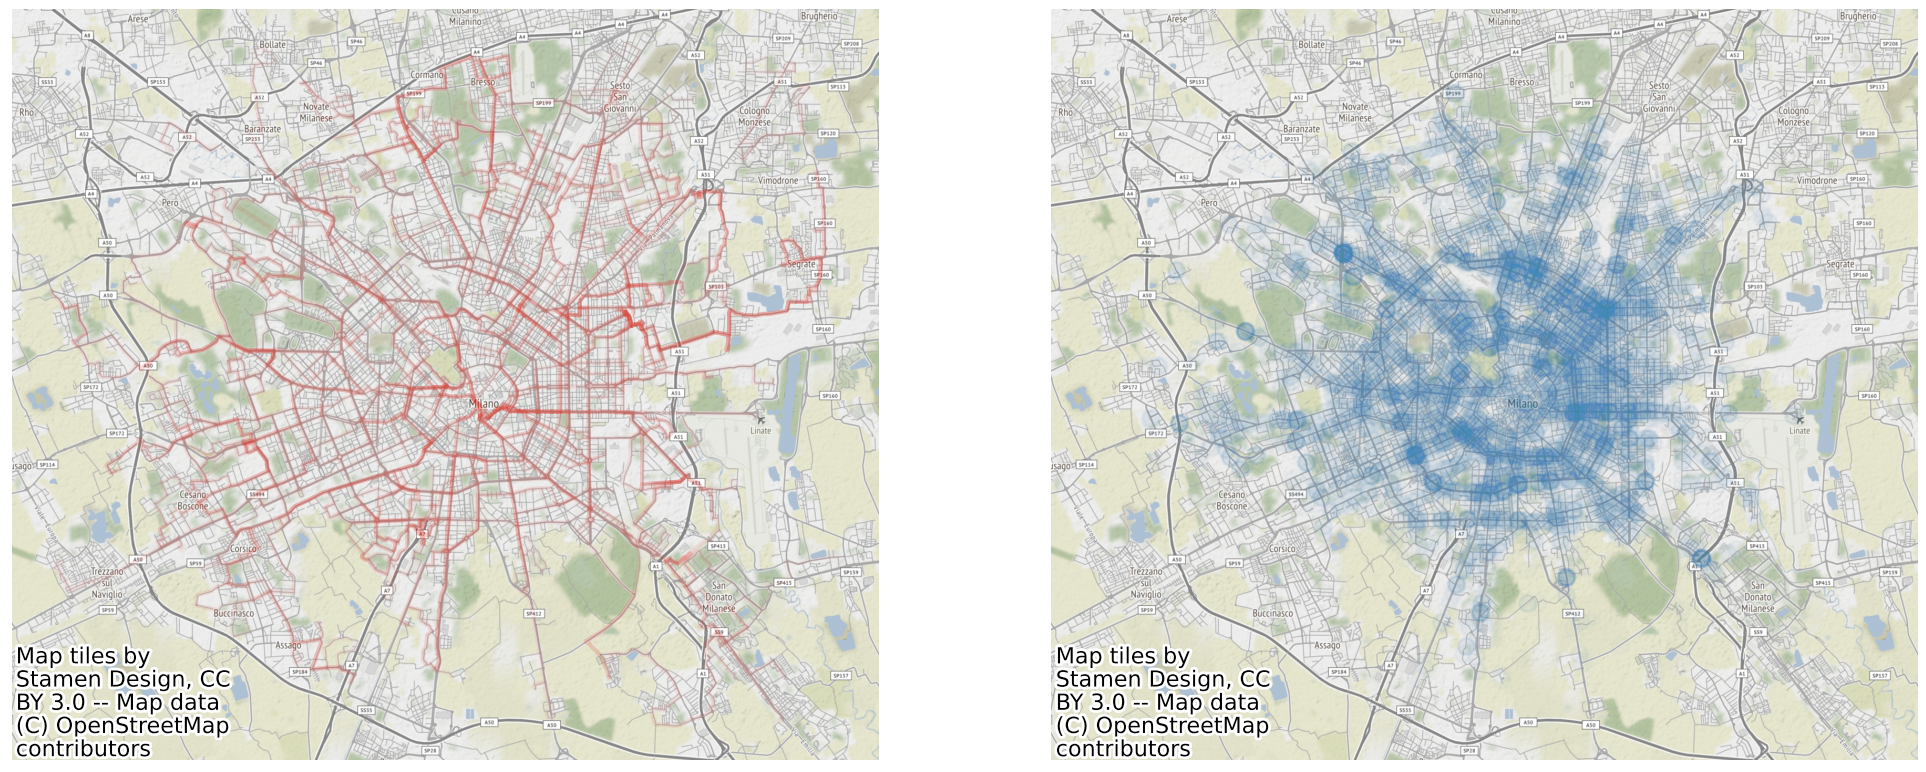
\includegraphics[width=\linewidth]{../src/atm/linee_atm.png}
    \caption{Linee Autobus e Tram a Milano}
    \label{fig:geo-trasporti}
\end{figure}

Affiancando le posizioni dei sinistri alle linee dei trasporti, 
non è possibile notare un collegamento preciso tra i due dataset. 
Sono presenti tuttavia alcune corrispondenze, come la zona dei Navigli 
e quella circostante a Corso Ventidue Marzo. 

Un fenomeno interessante, è la presenza di alcune strade con alta incidentalità, 
parallele a viali su cui viaggiano mezzi pubblici. 
Nella zona Navigli, in figura \ref{fig:navigli}, le vie 
interessate sono Viale Gian Galeazzo, Viale Beatrice D'Este, 
parallele a Viale Col di Lana e Viale Bligny. 
Lo stesso comportamento prosegue su Viale Gabriele D'Annunzio e Viale Gorizia e Coni Zugna, 
località vicine alle direttrici precedenti. 

\begin{figure}
    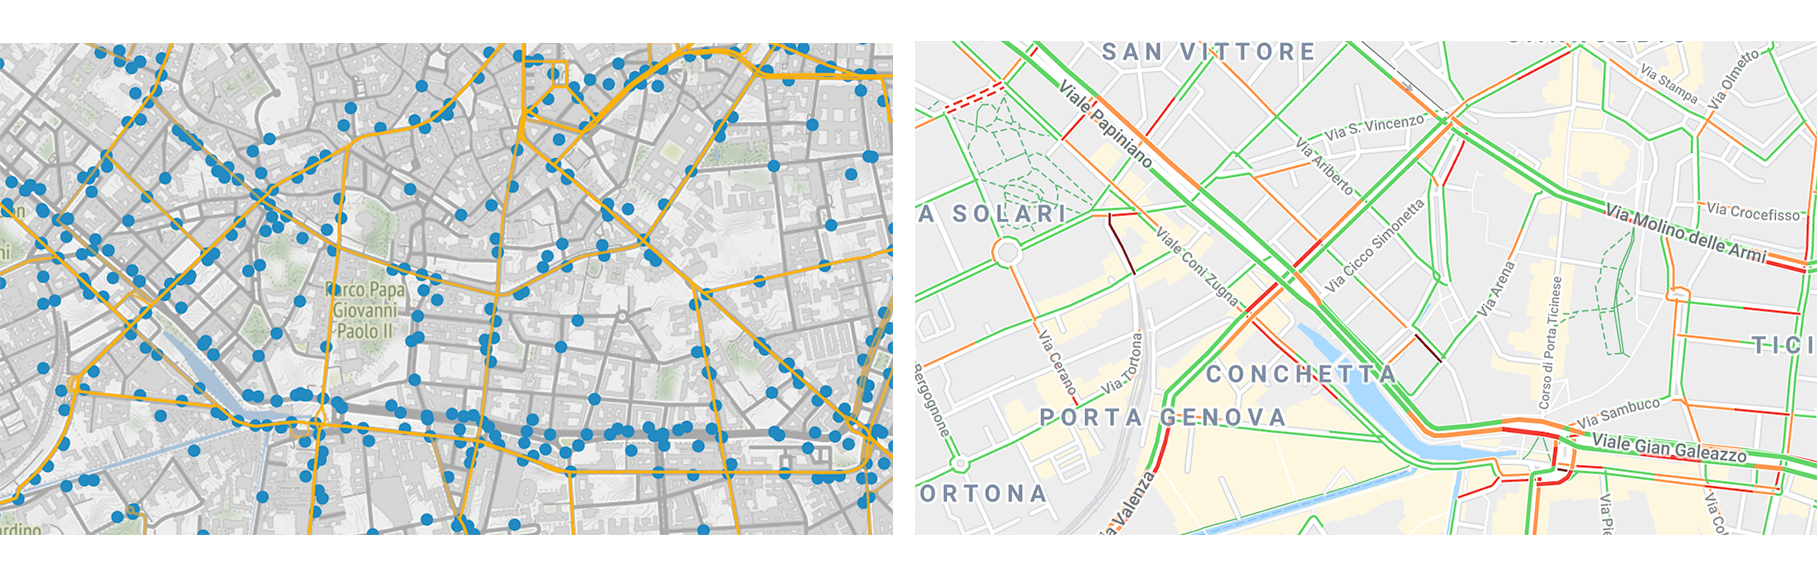
\includegraphics[width=\linewidth]{../src/atm/navigli.png}
    \caption{Linee dei trasporti pubblici e condizioni di traffico nella zona Navigli}
    \label{fig:navigli}
\end{figure}

Anche tra Viale Bianca Maria e Viale Premuda, nella mappa \ref{fig:22-marzo} si può 
notare lo stesso fenomeno, in prossimità di corso Ventidue Marzo. 

\begin{figure}
    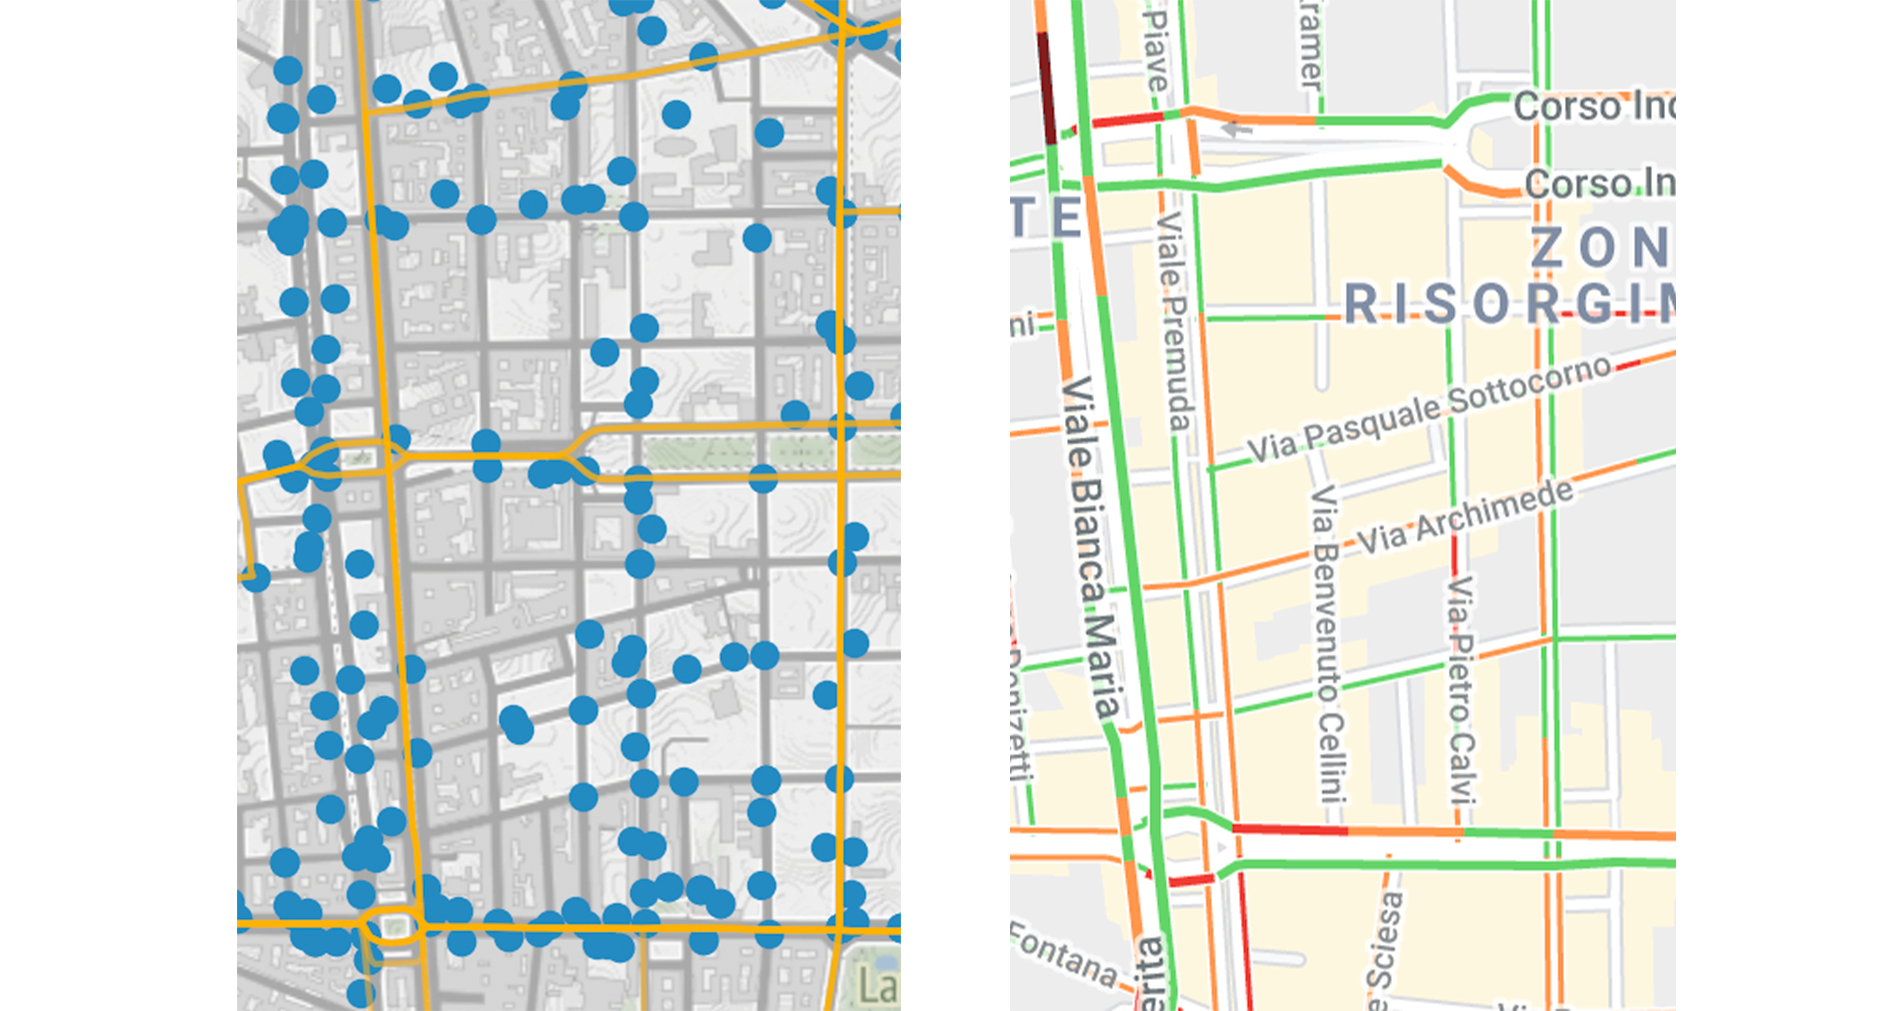
\includegraphics[width=\linewidth]{../src/atm/22_marzo.png}
    \caption{Linee dei trasporti pubblici e condizioni traffico vicino a Corso Ventidue Marzo}
    \label{fig:22-marzo}
\end{figure}

Le immagini, 
del contenenti indicazioni sul traffico, affiancate alle mappe, 
sono state realizzate tramite le API di 
Google Maps. 
Va specificato che queste non offrono una stima ideale, poiché indicano 
il traffico in tempo reale e ciò non solo comporta imprecisione per l'orario, 
ma anche per 
la quarantena dovuta al Covid-19 che ha ridotto notevolmente il volume di automobili 
circolanti. 

Per confutare l'ipotesi iniziale, si sono utilizzati i dati ricavati 
nel capitolo precedente, 
cioè gli incidenti per chilometro quadrato, calcolati per ogni municipio di Milano. 
Nella zona dei Navigli, si è poi presa in considerazione la sezione 
nell'immagine sinistra 
della figura \ref{fig:zona-navigli-22marzo}, 
perché sono presenti molti incidenti in viale Papiniano e viale Beatrice d'Este, 
e un numero minore nella vie parallele sottostanti, su cui viaggiano 
trasporti pubblici. 

\begin{figure}
    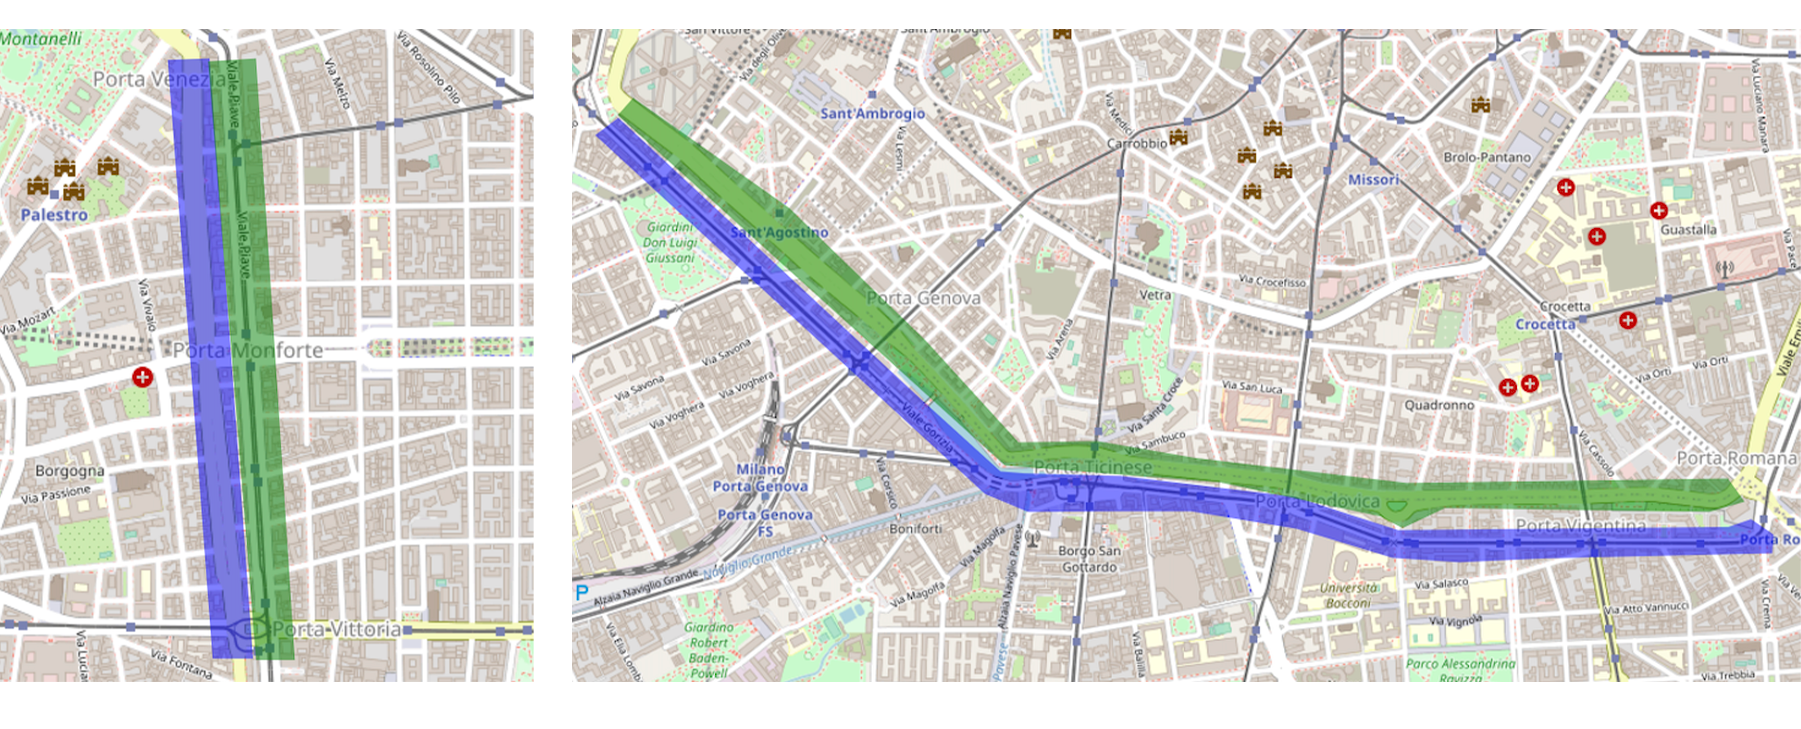
\includegraphics[width=\linewidth]{img_unite/zona_navigli_22marzo.png}
    \caption{Sezioni di Milano prese in considerazione per contare gli incidenti ai Navigli e nella zona di Corso Ventidue Marzo}
    \label{fig:zona-navigli-22marzo}
\end{figure}

\begin{code}
data = gp.read_file("dataset/zone_milano/zone.geojson").to_crs(epsg=3857)
autobus = data[data['name'] == "Navigli Autobus"]
street = data[data['name'] == "Navigli Incidenti"]

autobus_rect = geometry.Polygon(autobus['geometry'].iloc[0])
street_rect = geometry.Polygon(street['geometry'].iloc[0])

inc_a = 0
inc_s = 0
for point in incidenti['geometry']: 
    point = geometry.Point(point)

    if autobus_rect.contains(point): 
        inc_a += 1
        
    if street_rect.contains(point): 
        inc_s += 1
\end{code}

Il risultato, conferma che avvengono $167.09$ sinistri per chilometro quadrato
nel viale in cui sono presenti trasporti pubblici e, per quanto non sia nella media per la zona 
di appartenenza, è giustificabile in quanto si sono prese in considerazione solo le strade, 
e non le 
\quotestyle{zone morte}\footnote{Zone come parchi e edifici, dove non possono 
viaggiare automobili e non possono quindi avvenire incidenti}. 
Su Viale Papiniano e Beatrice D'Este, invece, dove non passa alcuna 
linea di trasporti pubblici, 
gli incidenti sono $289.32$, risultato ancora più alto rispetto a quello ottenuto 
nella zona di Loreto. 

\skipline
Nonostante si siano ricavati questi valori particolarmente alti, 
non è detto che il maggior numero di sinistri sia causato dall'assenza di una 
linea di autobus, 
in particolare, va tenuta in considerazione la topologia delle due vie parallele. 
La differenza principale tra Viale Bligny e Viale Beatrice d'Este è che, 
la prima è una via a due 
corsie per senso di marcia, mentre il secondo è un viale a due 
carreggiate\footnote{Carreggiata: la parte della strada destinata allo scorrimento dei veicoli, 
delimitata da una striscia continua o da un paracarro} 
separate da una zona non attraversabile da automobili. 
Dunque è ovvio che la maggior parte dei conducenti preferirà un viale ad alta velocità 
rispetto a una via dove è possibile rimanere incolonnati per la presenza di una sola 
corsia, e dove si è rallentati dalla presenza di autobus o tram. 

Lo stesso procedimento è stato realizzato per Corso Ventidue Marzo, le zone utilizzate sono 
raffigurate nell'immagine destra della figura \ref{fig:zona-navigli-22marzo}. 

In questo caso, per viale Bianca Maria, dove non è presente una linea di trasporti pubblici, 
il numero di incidenti è $254.31$, mentre per viale Premuda per cui passa una linea tranviaria, 
il valore ottenuto dallo stesso calcolo scende a $93.96$. 

Anche per questa zona, le due vie prese in considerazione sono molto diverse. 
Viale Premuda dispone di due carreggiate separate, ognuna con una corsia e un solo senso 
di marcia, dove sono parcheggiate automobili su entrambi i lati, e la velocità delle 
vetture non deve essere particolarmente elevata. 
Allo stesso modo, su Viale Bianca Maria, le carreggiate sono separate, tuttavia queste 
hanno due, e in alcuni punti tre corsie ciascuna. 

Va sottolineato che le strade prese in considerazione hanno differenze sostanziali, 
e che probabilmente, il numero maggiore di incidenti su viali più ampi sia dovuto al 
volume di traffico più elevato. 
D'altro canto, è più che possibile che una parte dei conducenti, 
come quelli con maggiore esperienza di guida in grandi città, evitino di proposito 
strade con mezzi pubblici.

%\clearpage
\subsection{Il pavé a Milano influisce in qualche modo sull'incidentalità?}
\todo{ATOK}

Tra le domande poste nell'introduzione, una particolarmente interessante è quella 
sull'influenza del pavé sull'incidentalità. 

Il primo dataset, con cui si è tentato di approssimare le vie in pavé, è stato quello 
delle linee tranviarie. 
Confrontando queste e la cartina di Urbanfile, nell'immagine \ref{fig:tram-pave-milano}, 
è possibile notare alcune somiglianze, come tra viale Sabotino e via 
Alessandro Manzoni, tuttavia la maggior parte delle linee tranviarie segnate 
passano su asfalto. 
Inoltre, in alcune tratte, come viale Premuda, i tram viaggiano su una carreggiata separata, 
che deve avere influenza minore sugli incidenti della zona. 

\begin{figure}
    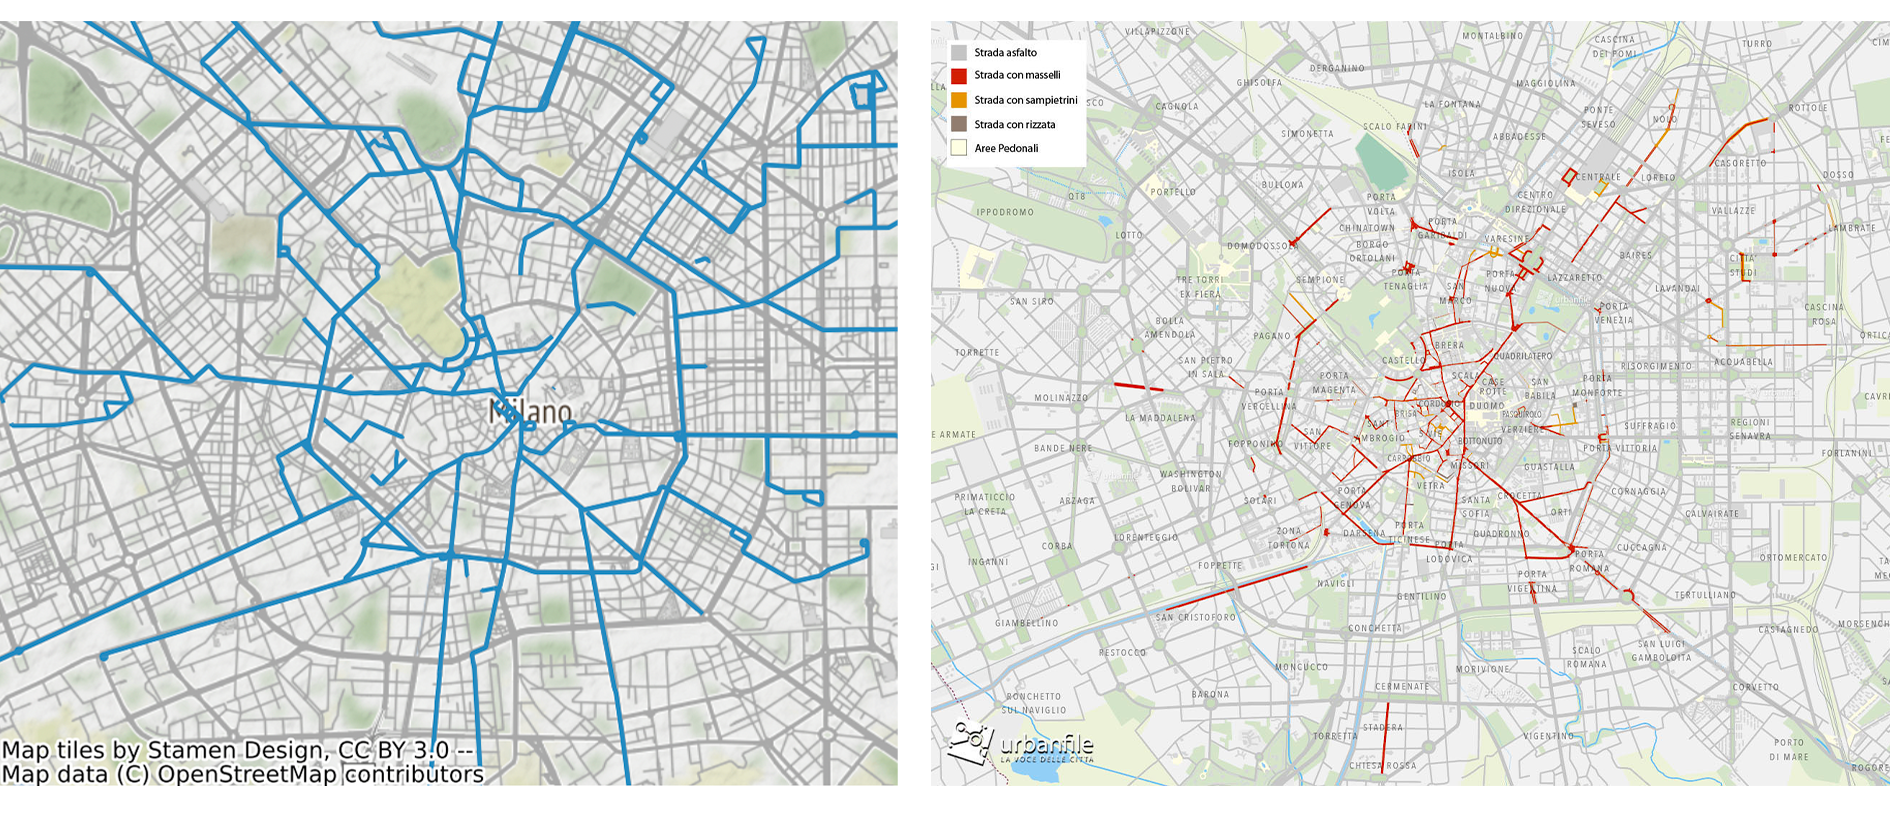
\includegraphics[width=\linewidth]{../src/tram/tram_milano.png}
    \caption{Cartina con strade in pavé e linee tranviarie a Milano}
    \label{fig:tram-pave-milano}
\end{figure}

Viste le basse somiglianze tra la mappa di Urbanfile e le linee dei trasporti pubblici, 
per creare un dataset, si sono convertite le vie principali della cartina trovata 
in geojson. 
Nella sezione sull'origine dei dati, si è parlato di come è stato possibile ricavare 
un tracciato con la maggior parte delle strade in pavé a Milano e, allo stesso modo, 
anche un campione di tratte asfaltate con caratteristiche simili. 

Il risultato è visibile nella mappa sulla sinistra dell'immagine \ref{fig:mappa-pave}. 

\begin{figure}
    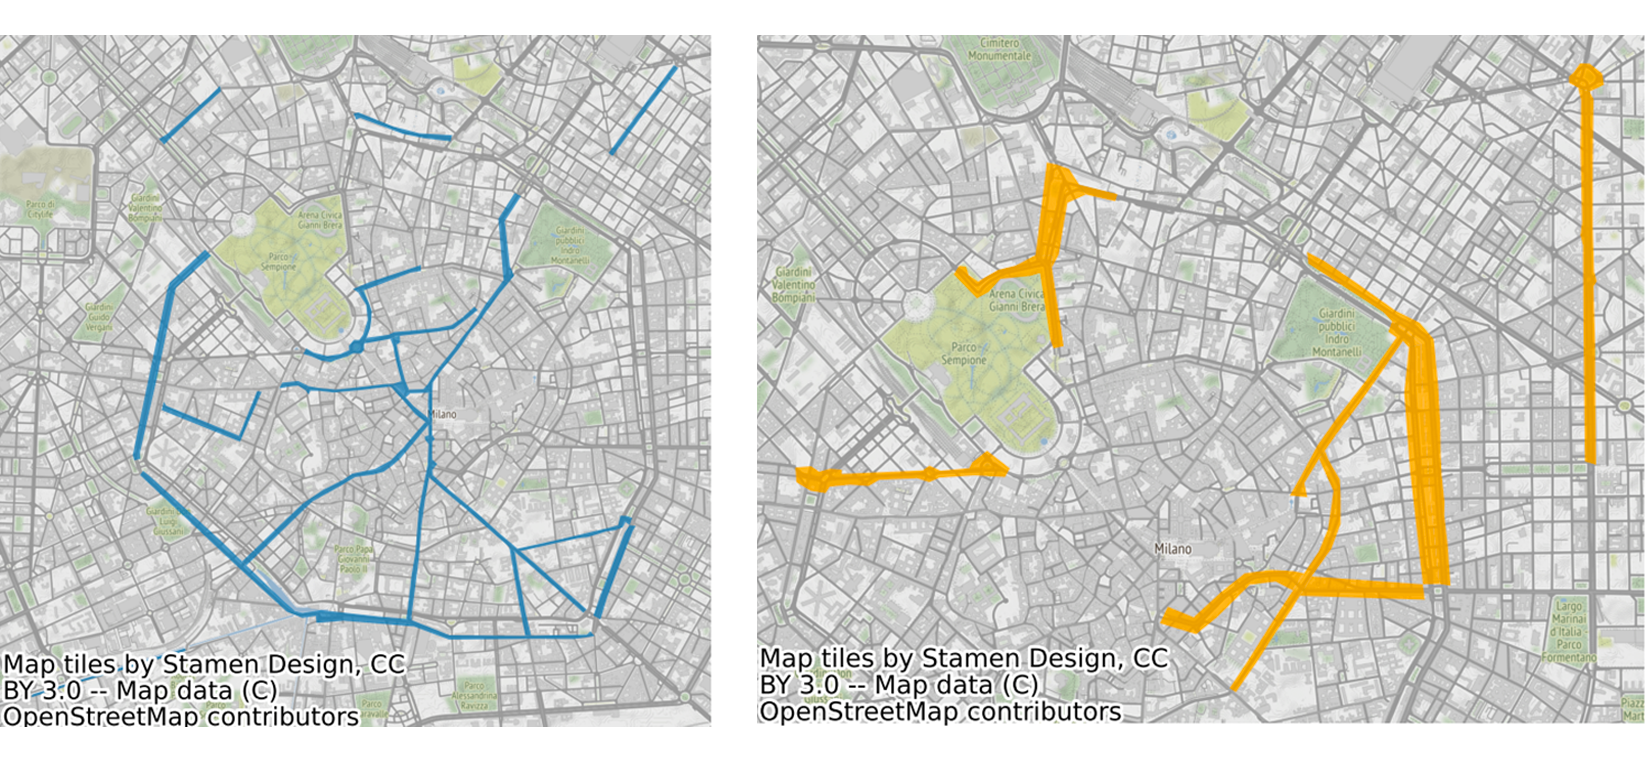
\includegraphics[width=\linewidth]{img_unite/mappa_pave_asfalto.png}
    \caption{Principali strade a Milano in pavé e campione simile con zone asfaltate}
    \label{fig:mappa-pave}
\end{figure}

Una volta creata l'area delle strade in pavé, è possibile calcolare quanti 
incidenti avvengono in questi luoghi e confrontarlo con il numero di sinistri 
nei viali asfaltati. 

\begin{code}
inc_in_pave = 0
for rect in pave['geometry']: 
    rect = geometry.Polygon(rect)

    for point in incidenti['geometry']: 
        if rect.contains(geometry.Point(point)): 
            inc_in_pave += 1

area_pave = 0
for rect in pave['geometry']: 
    area_pave += geometry.Polygon(rect).area

incidenti_per_km = inc_in_pave * 10**6 / area_pave
\end{code}

La quantità di incidenti per chilometro quadrato su pavé è $229.45$, 
questo è un valore particolarmente alto, anche se viene confrontato con il numero di 
sinistri nel centro storico, cioè circa $120$. 
Tuttavia, bisogna tenere in considerazione che il dataset appena creato 
contiene solamente strade, senza alcuna \quotestyle{zona morta}, 
come edifici o parchi, mentre l'area del centro storico, 
si riferisce a tutto il territorio, che si traduce in una frazione con 
denominatore maggiore. 

Per ovviare a questo problema, si è selezionato il campione di strade asfaltate, 
prese nella stessa zona di Milano, per mantenere le quantità di traffico il più 
costante possibile. 
Inoltre, per lo stesso motivo, la superficie totale dei due dataset è simile. 
Questi tracciati sono raffigurati nella mappa destra in figura \ref{fig:mappa-pave}. 

Nonostante si sia tentato di tenere i due campioni il più simili 
possibili, in quello delle strade asfaltate sono stati presi vari tratti 
provenienti dalla circonvallazione interna e altre zone molto trafficate, 
mentre l'insieme in pavé contiene, per mancanza di altri dati, 
molti viali provenienti dal centro storico, inevitabilmente 
meno trafficati. 

Con lo stesso calcolo realizzato per le strade in pavé, risulta che 
il numero di incidenti per 
chilometro quadrato, nel campione creato, sia uguale a $220.89$. 

Per quanto il risultato dell'analisi sulle strade in pavé abbia restituito un valore di 
sinistri maggiore, non sarebbe sbagliato considerare i due numeri vicini. 
Per rendere le informazioni più precise, disponendo di dati sulla 
posizione degli incidenti in più annate, e sapendo che il pavé è stato 
rimosso da alcuni viali, sarebbe possibile eseguire un confronto 
sulla stessa direttrice, avendo come unica variabile il cambio di pavimentazione. 

%\clearpage
\subsection{Incidenti e Autovelox}
\todo{ATOK}

Per sapere se la presenza di autovelox abbia influenza sugli incidenti, 
bisognerebbe innanzitutto sapere quando sono stati posizionati i dispositivi, e solo 
a quel punto, avendo dati sui sinistri prima e dopo l'installazione, sarebbe 
possibile trarre conclusioni. 

Informazioni sul posizionamento di alcune telecamere sono reperibili per 
l'anno 2014, e sono visualizzabili nella tabella \ref{ztl-milano}. 
Tuttavia la localizzazione degli incidenti 
è disponibile solo per il 2016, in quanto Istat non ha rilasciato 
le coordinate di sinistri in altre annate. 

\todo{atrent: tutta questa sezione va resa più ipotetica perché non hai 
informazioni "causali" lelepado: ho aggiunto la parte successiva 
per spiegare meglio cosa manca}

Non disponendo delle informazioni sul comportamento delle vetture 
precedentemente all'installazione degli autovelox, 
non è possibile calcolare un contesto valido per quanto riguarda 
i sinistri prima del 2016. 
Nonostante ciò, avendo i dati riferiti al 2016, e le posizioni dei tutor 
già presenti in quell'anno, è possibile eseguire comunque il procedimento corretto, 
se pur con dei dati non coerenti, per vedere se gli 
autovelox abbiano un qualche tipo di effetto sugli incidenti.

Nella sezione seguente, dunque, si assume di disporre di due dataset di sinistri, uno 
precedente e uno successivo al 2014, e di eseguire i calcoli su entrambi gli insiemi, 
osservando le eventuali differenze presenti nei risultati ottenuti.

\begin{figure}
    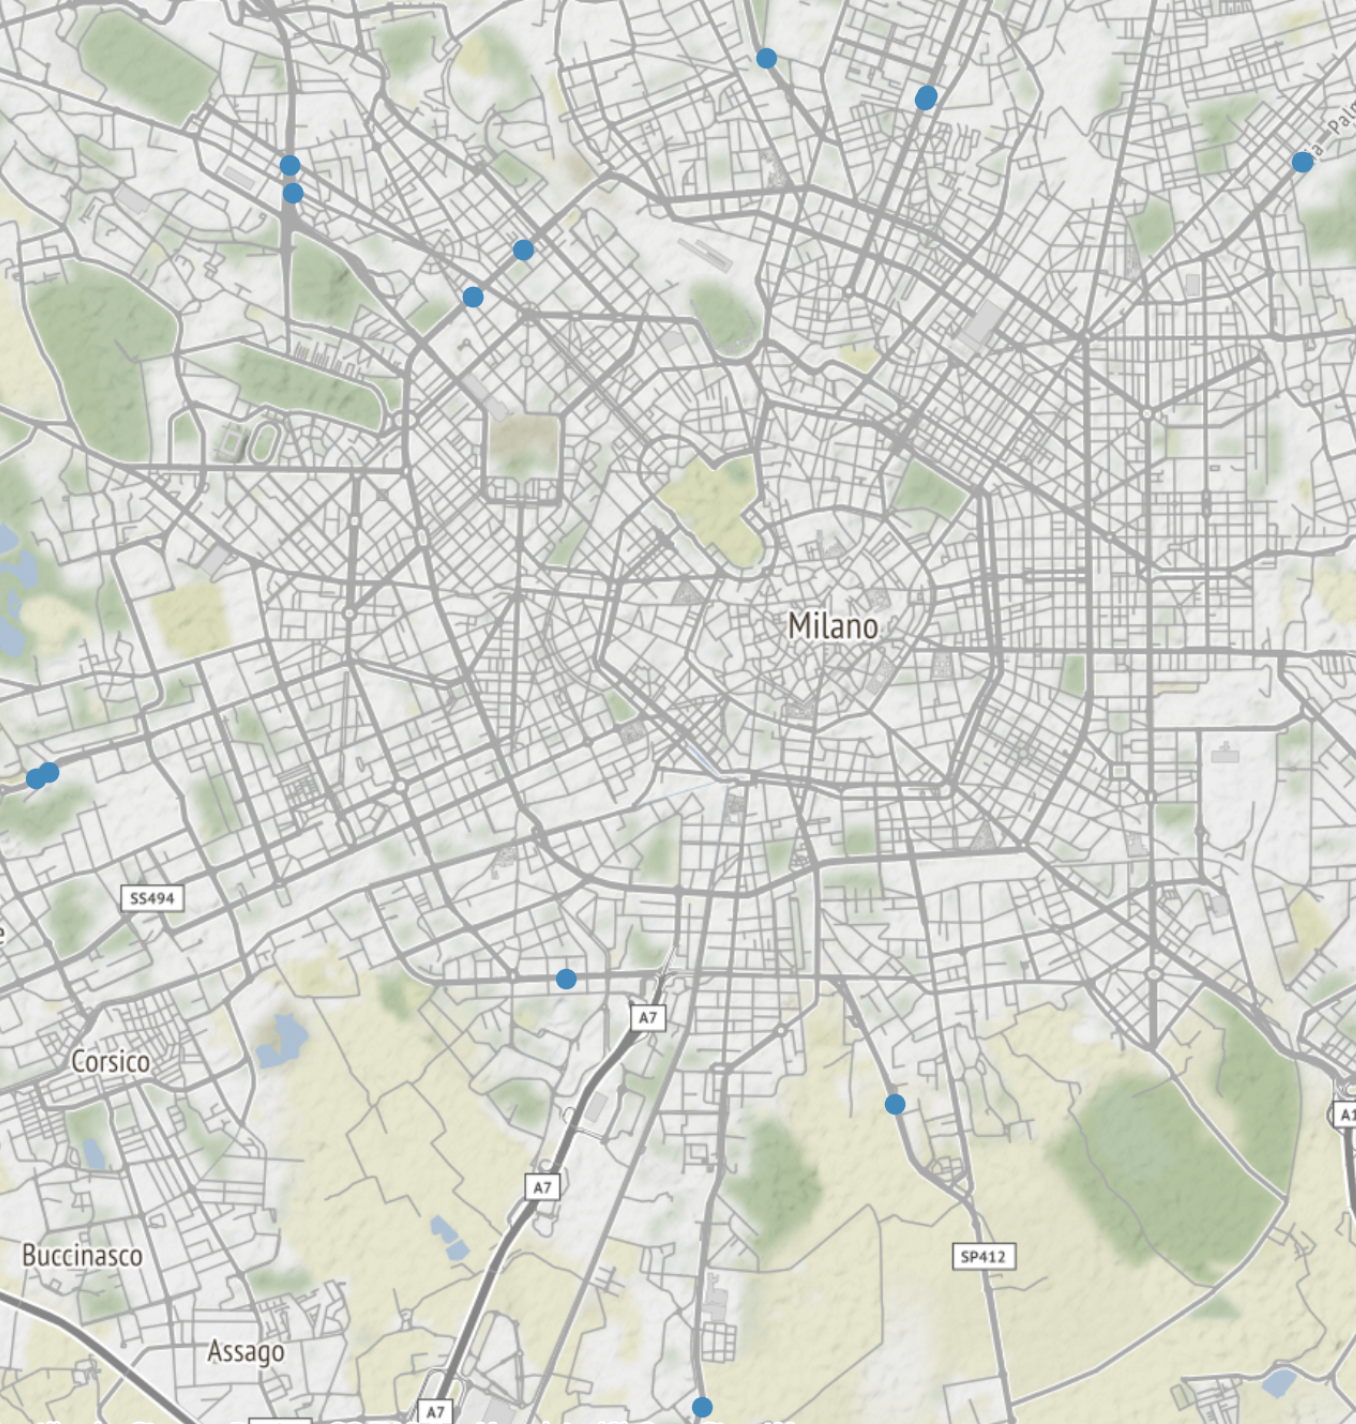
\includegraphics[width=\linewidth]{../src/autovelox/autovelox_2014.png}
    \caption{Autovelox installati nel 2014 e quelli il cui anno di installazione è ignoto}
    \label{fig:autovelox-indici}
\end{figure}

Conoscendo il nome della via in cui sono stati installati gli autovelox nel 2014, 
è possibile ricondursi alla posizione effettiva di questi sulla mappa. 
Per fare ciò, la soluzione più veloce è stata quella di enumerare tutte le coordinate presenti 
nel dataset dei dispositivi trovato, 
e confrontarli con le vie della tabella, salvando quelle che coincidono. 
Il risultato è rappresentato nella cartina sul lato sinistro della 
figura \ref{fig:autovelox-indici}. 

\begin{code}[language=Python]
path = "dataset/autovelox/autovelox_milano.geojson"
autovelox = gp.read_file(path).to_crs(epsg=3857)
layer_autovelox = autovelox.plot(figsize=(11,9), color="red")
    
index = 0
for lat, lon in geo_utils.parse_geojson_point_list(autovelox['geometry'].astype(str)):
    layer_autovelox.text(lat, lon, s=index)
    # si aggiunge un label per ogni punto
    index += 1
    
cx.add_basemap(ax=layer_autovelox)
plt.show()
\end{code}

Per quanto non si disponga delle informazioni sui sinistri prima e dopo dell'installazione, 
è comunque possibile sovrapporre i dataset, per vedere se gli autovelox 
hanno un qualche tipo di effetto sugli incidenti, visto che i dati 
localizzati sono successivi al posizionamento delle telecamere. 

\begin{figure}
    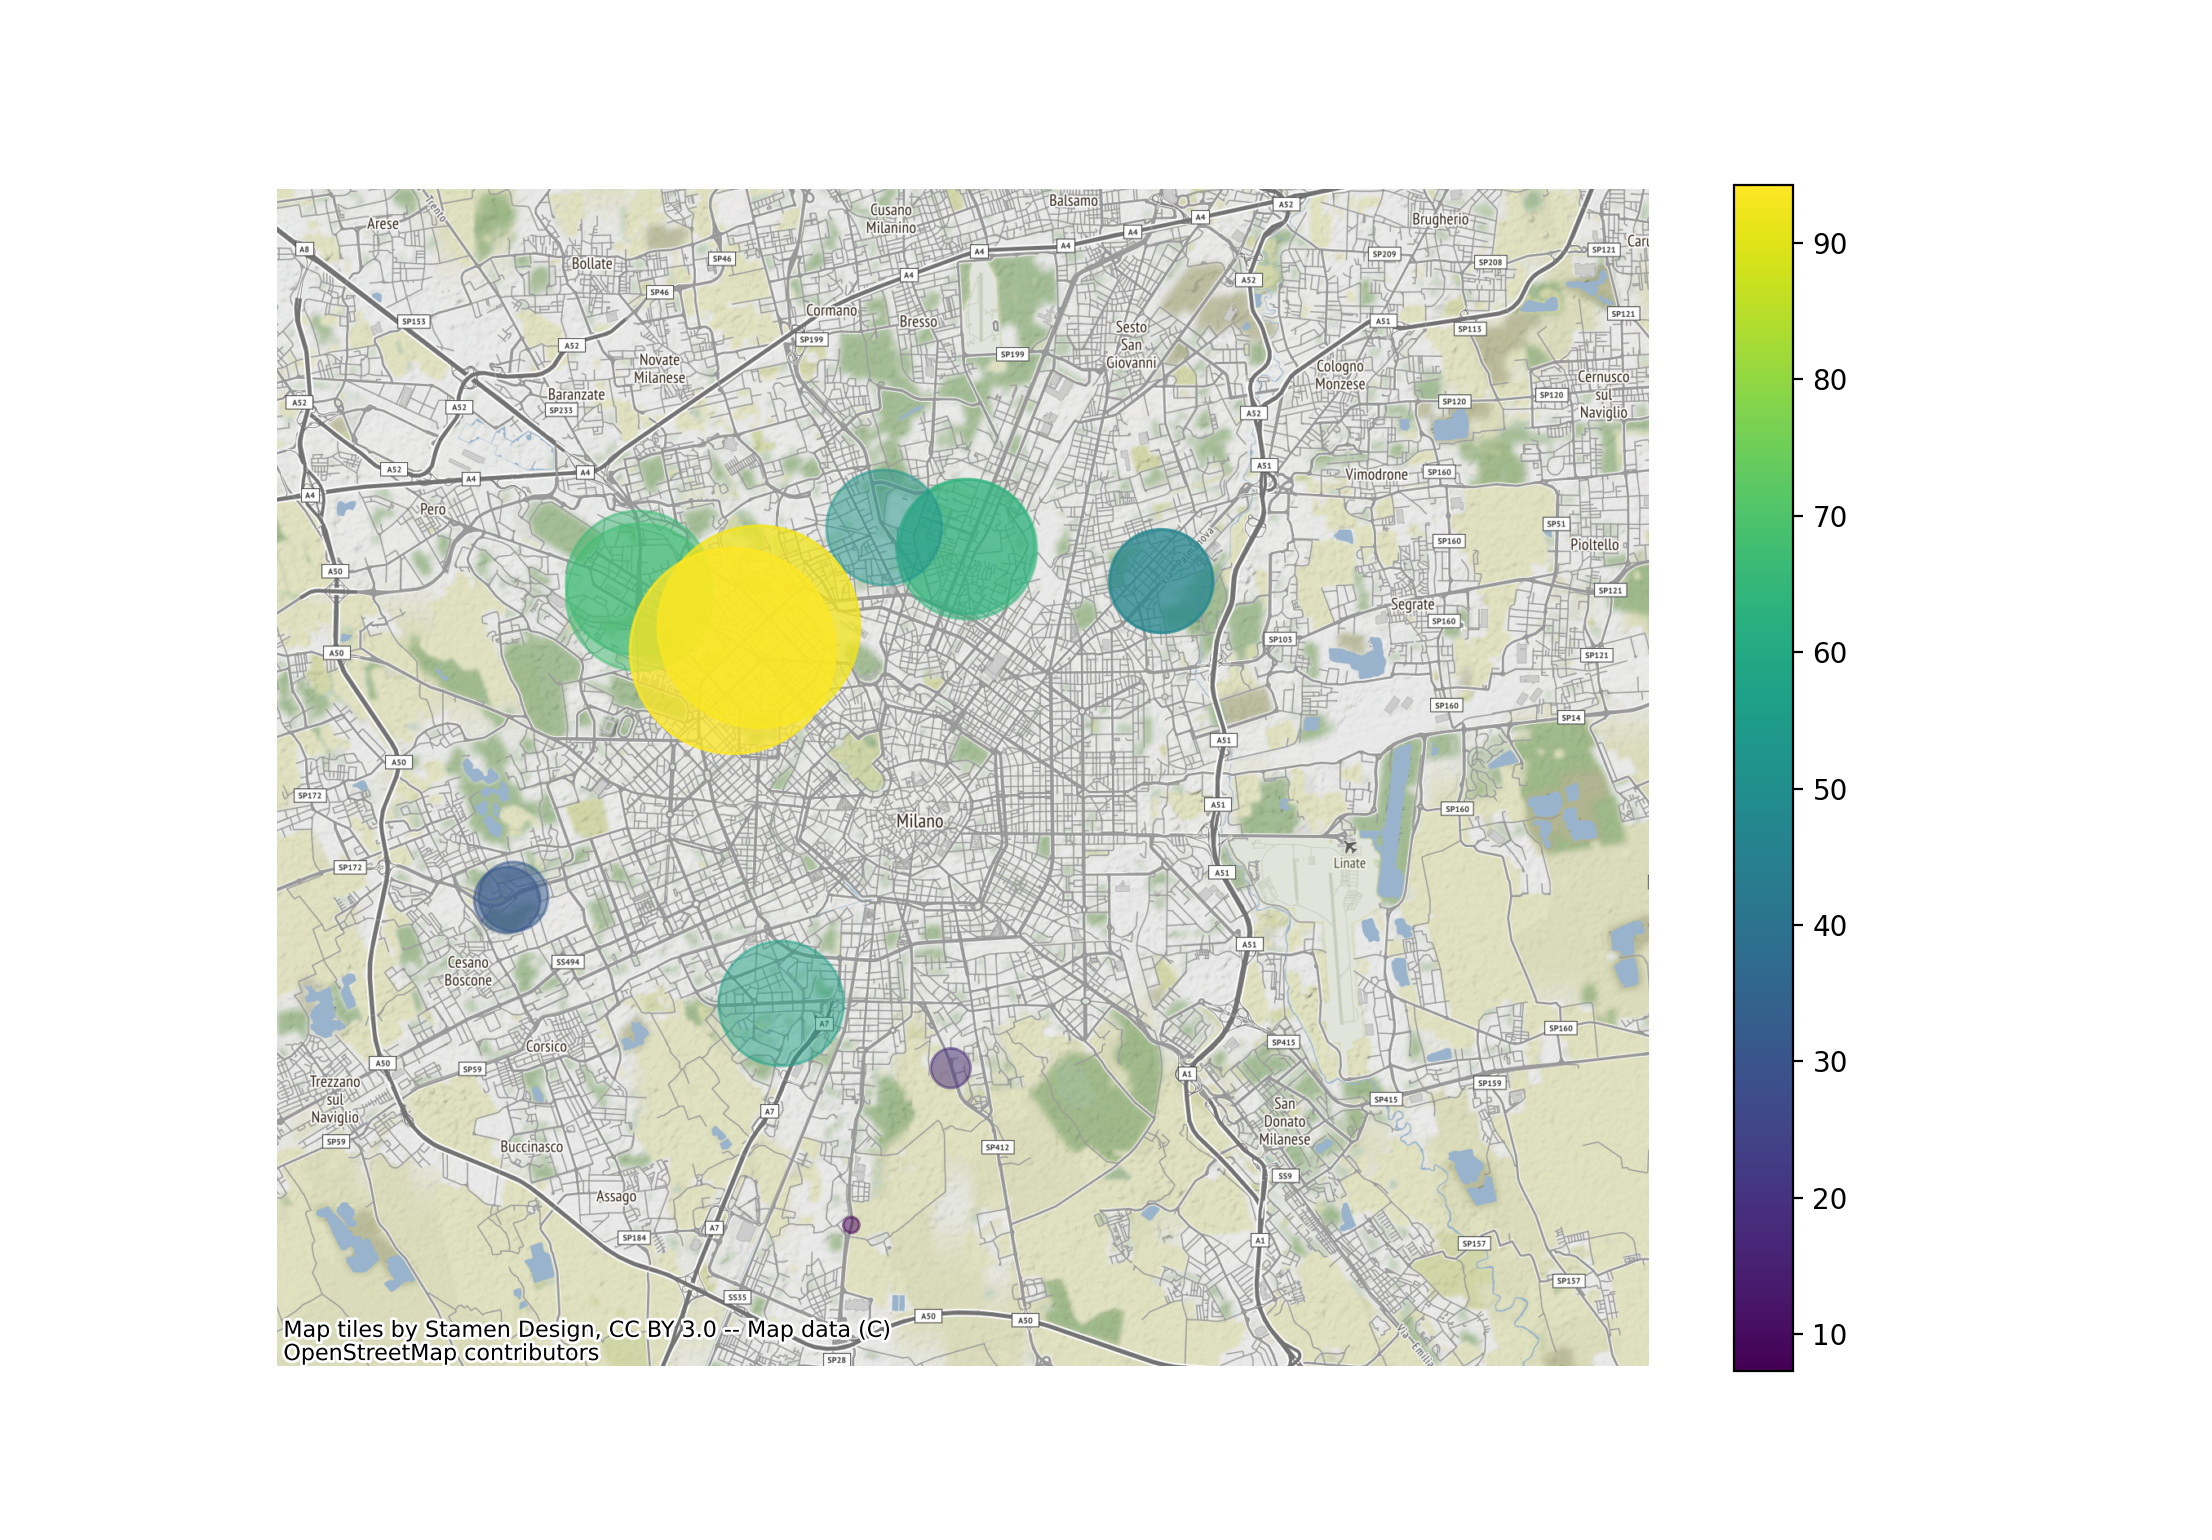
\includegraphics[width=\linewidth]{../src/autovelox/autovelox_incidenti.png}
    \caption{Autovelox e Incidenti a Milano}
    \label{fig:autovelox-incidenti}
\end{figure}

La mappa \ref{fig:autovelox-incidenti} è stata realizzata contando 
gli eventi avvenuti nel raggio di un chilometro da ogni autovelox. 
Va precisato che le \quotestyle{bolle} non indicano il raggio di conteggio degli incidenti, ma 
il numero dei sinistri trovati. 
La colorazione dei cerchi è stata aggiunta per 
rendere la cartina più leggibile, la sua interpretazione poteva, infatti, risultare 
difficoltosa osservando solo l'ampiezza di questi. 

\begin{center}
    \def\arraystretch{1.5}% 
    \begin{tabular}{ |c|c|c|c| }
        \hline
        Autovelox & Totali & Per $Km^2$ & Per zona \\ 
        \hline
        \rowcolor{TableGray}
        V. F. Testi d. perif.\footnotemark[1]   &   194 &   61.78   &   69.52 \\
        V. F. Testi d. centro                   &   202 &   64.33   &   69.52 \\
        \rowcolor{TableGray}
        C. Ghisallo d. centro\footnotemark[2]   &   208 &   66.24   &   44.3 \\
        C. Ghisallo d. perif.                   &   212 &   67.51   &   44.3 \\
        \rowcolor{TableGray}
        V. Fermi                                &   166 &   52.86   &   51.25 \\
        V. Parri d. perif.                      &    95 &   30.25   &   43.63 \\
        \rowcolor{TableGray}
        V. Parri d. centro                      &   100 &   31.84   &   43.63 \\
        V. Famagosta                            &   180 &   57.32   &   43.63 \\
        \rowcolor{TableGray}
        V. Missaglia d. centro                  &   23  &    7.32   &   27.54 \\
        V. Ferrari                              &   57  &   18.15   &   44.3 \\
        \rowcolor{TableGray}
        V. Monte Ceneri d. Serra                &   291 &   92.67   &   44.3 \\
        V. Monte Ceneri d. Lugano               &   290 &   92.35   &   44.3 \\
        \rowcolor{TableGray}
        V. Serra d. Lotto                       &   296 &   94.26   &   44.3 \\
        V. Serra d. Monte Ceneri                &   296 &   94.26   &   44.3 \\
        \rowcolor{TableGray}
        V. Palmanova d. perif.                  &   149 &   47.45   &   59.79 \\
        V. Palmanova d. centro                  &   149 &   47.45   &   59.79 \\
        \hline
    \end{tabular}
\end{center}

\footnotetext[1]{Viale Fulvio Testi}
\footnotetext[2]{Cavalcavia del Ghisallo}

Una volta trovati i sinistri totali presenti nel raggio, 
è possibile calcolare il numero di eventi avvenuti per chilometro quadrato, 
in base all'area utilizzata. 
Alla tabella degli autovelox sono aggiunte tre colonne, contenenti gli incidenti totali, 
quelli per chilometro quadrato e quelli registrati nella zona municipale corrispondente. 

\begin{code}
autovelox_2014['incidenti_vicini'] = gp.GeoSeries(df)
autovelox_2014['incidenti_pesati'] = autovelox_2014['incidenti_vicini'] / 3.14
\end{code}

Quest'ultima colonna, in particolare, è divisa per $3.14$ perché l'area del cerchio 
è data dalla formula sottostante: 

\begin{center}
    $Area\, = \pi * r^2$
\end{center}

Poiché si sta utilizzando un raggio di un chilometro, e si vuole ottenere il 
numero di incidenti per chilometro quadrato, l'area ottenuta è $3.14$. 

Per facilitare la lettura della tabella precedente, nella figura \ref{fig:confronto-autovelox} 
è visibile sia il confronto tra i sinistri vicino a autovelox, 
sia tra quelli che avvengono nel rispettivo municipio. 
In alcuni casi, il numero di incidenti sembra essere ridotto dalla presenza 
della telecamera,  
tuttavia nella maggior parte delle zone, e soprattutto in prossimità di Viale Serra e 
Viale Monte Ceneri, questo valore è particolarmente più alto di 
quello della zona municipale. 

\begin{figure}
    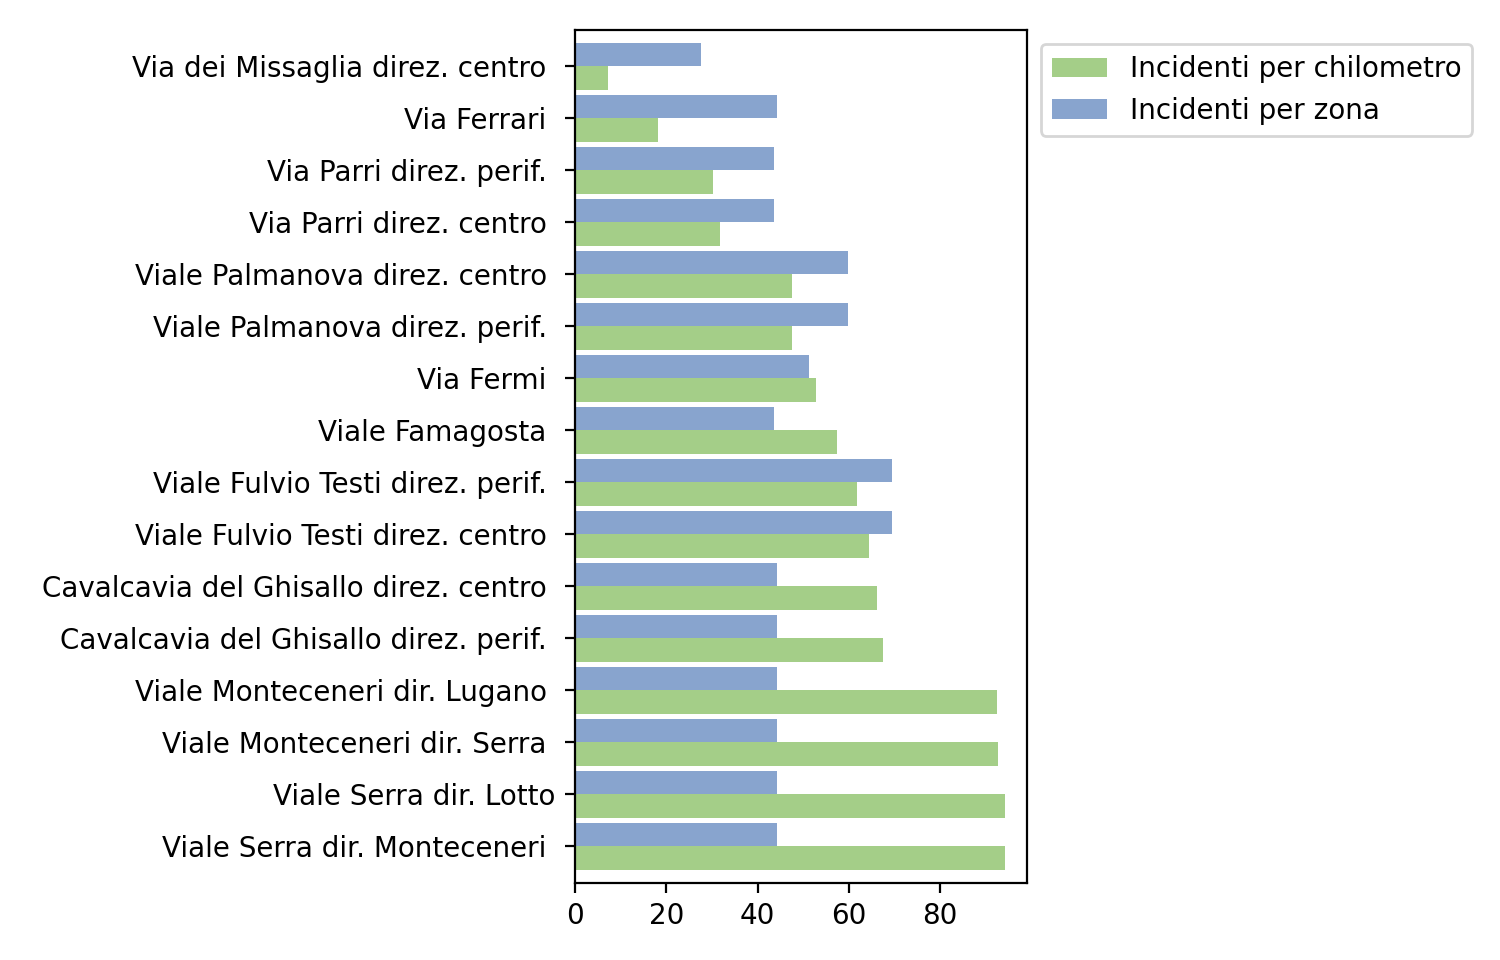
\includegraphics[width=\linewidth]{../src/autovelox/conclusioni_autovelox.png}
    \caption{Incidenti vicino a autovelox rispetto a quelli per zona di Milano}
    \label{fig:confronto-autovelox}
\end{figure}

\begin{code}
incremento_percentuale_totale = 0
for km, zona in zip(data['Incidenti per chilometro'], data['Incidenti per zona']): 
    incremento_percentuale = (km - zona) * 100 / zona
    incremento_percentuale_totale += incremento_percentuale

print(incremento_percentuale_totale)
\end{code}

Sarebbe interessante poter visualizzare, tramite un solo valore numerico, 
l'incremento (o il decremento) globale, degli incidenti in zone vicine a 
autovelox\footnote{Si tenta di capire, con un solo numero, se la presenza di 
telecamere nella zona aumenta o diminuisce il numero di sinistri}. 
A causa delle zone menzionate in precedenza, che alzano di molto la media di sinistri, 
in prossimità di telecamere si ha un aumento di 
incidenti del $329.6$ \%. 
Tuttavia, nel caso in cui si considerino 
outlier\footnote{In un campione di osservazioni, un outlier è un valore anomalo, 
particolarmente distante dagli altri dati disponibili \cite{PROB_E_STATISTICA:1}} 
i Viali Serra e Monte Ceneri, si ha invece un decremento generale del $113.6$ \%. 

Va comunque sottolineato che, non avendo informazioni sufficienti a calcolare una tendenza 
precedente all'installazione dell'autovelox, non si ha modo di sapere se questi abbiano un 
effetto positivo o negativo sull'incidentalità. 
Con il rilascio di nuovi dataset contenenti le coordinate di sinistri, 
possibilmente riferiti ad annate antecedenti al 2014, sarebbe possibile realizzare 
una stima con informazioni precedenti e 
successive al posizionamento delle telecamere. 


%\clearpage
\section{Dati Istat su veicoli}

%\clearpage
\subsection{Le tipologie di veicoli che commettono incidenti dipendono dalla conformazione della strada?}
\todo{atrent: non avevo detto di riformulare il titolo? lelepado: cambiato - atrent: rivediamoli TUTTI insieme}
\todo{ATOK}

Una prima analisi che è possibile realizzare, utilizzando il dataset Istat è, 
per quanto riguarda i veicoli, 
come la composizione di questi cambia al cambiare del tipo di strada. 
In altre parole, la percentuale, ad esempio, di autotreni sul totale dei veicoli 
in circolazione è diversa sulle autostrade rispetto alle strade provinciali?

\begin{code}[language=Python]
# Dove 1,2,3 sono gli ID dei diversi tipi di strade urbane, 
# mentre 4,5,6 gli ID delle strade extraurbane

strade_urbane = data[(data['localizzazione_incidente'] == 1) | (data['localizzazione_incidente'] == 2) | (data['localizzazione_incidente'] == 3)]['tipo_veicolo_a']
strade_extraurbane = data[(data['localizzazione_incidente'] == 4) | (data['localizzazione_incidente'] == 5) | (data['localizzazione_incidente'] == 6)]['tipo_veicolo_a']
\end{code}

Il grafico \ref{fig:differenza-strade} rappresenta quali sono le categorie di veicoli 
coinvolte con più frequenza in sinistri, per tre tipi di strade diverse, strade urbane, 
extraurbane e autostrade. 
Le percentuali sono calcolate per gruppo, quindi, sommando 
tutte le righe di \columnstyle{Autostrade}, si ottiene $1.0$. 

\begin{figure}
    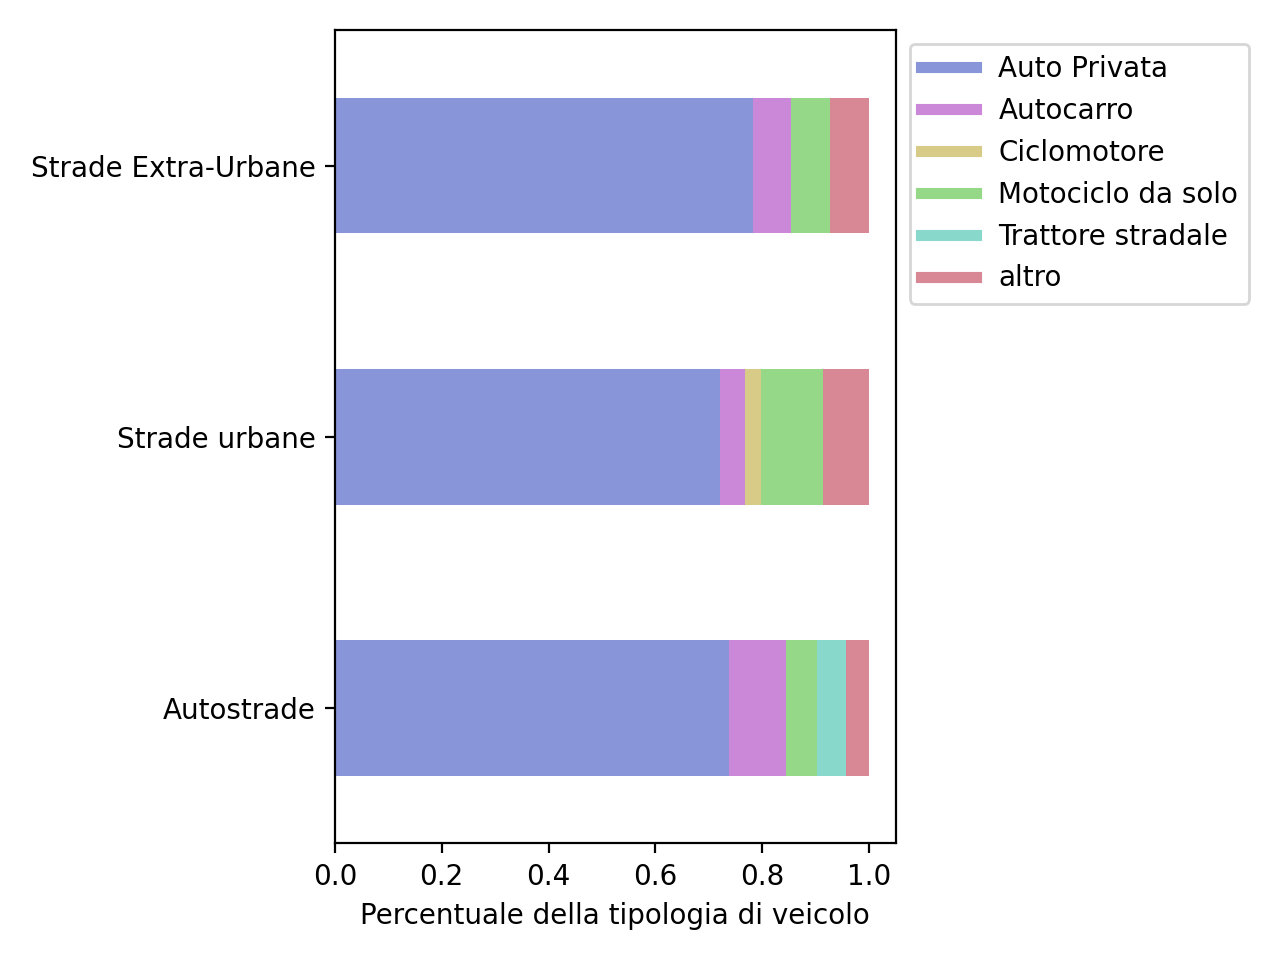
\includegraphics[width=\linewidth]{../src/incidenti/incidenti_senza_coords/tipo_veicoli/differenza_strade.png}
    \caption{Incidenti per tipo di veicolo nel 2018}
    \label{fig:differenza-strade}
\end{figure}

Possiamo quindi, notare che le auto private sono di gran lunga il tipo di veicolo 
maggiormente coinvolto in incidenti su ogni categoria di strada. 
I motocicli invece subiscono sinistri soprattutto su strade urbane.
Nel caso degli autocarri, si ha invece una bassa percentuale nelle strade 
urbane, mentre il volume di questa tipologia aumenta sulle autostrade. 

Visto che le auto private causano oltre tre quarti degli 
incidenti in ogni categoria di strada,  
si è deciso di ometterle, per avere una rappresentazione più 
precisa delle tipologie di veicoli che ricorrono con minore frequenza. 
I risultati sono mostrati, per l'anno 2018, 
nella figura \ref{fig:differenza-strade-no-auto}. 

\begin{figure}
    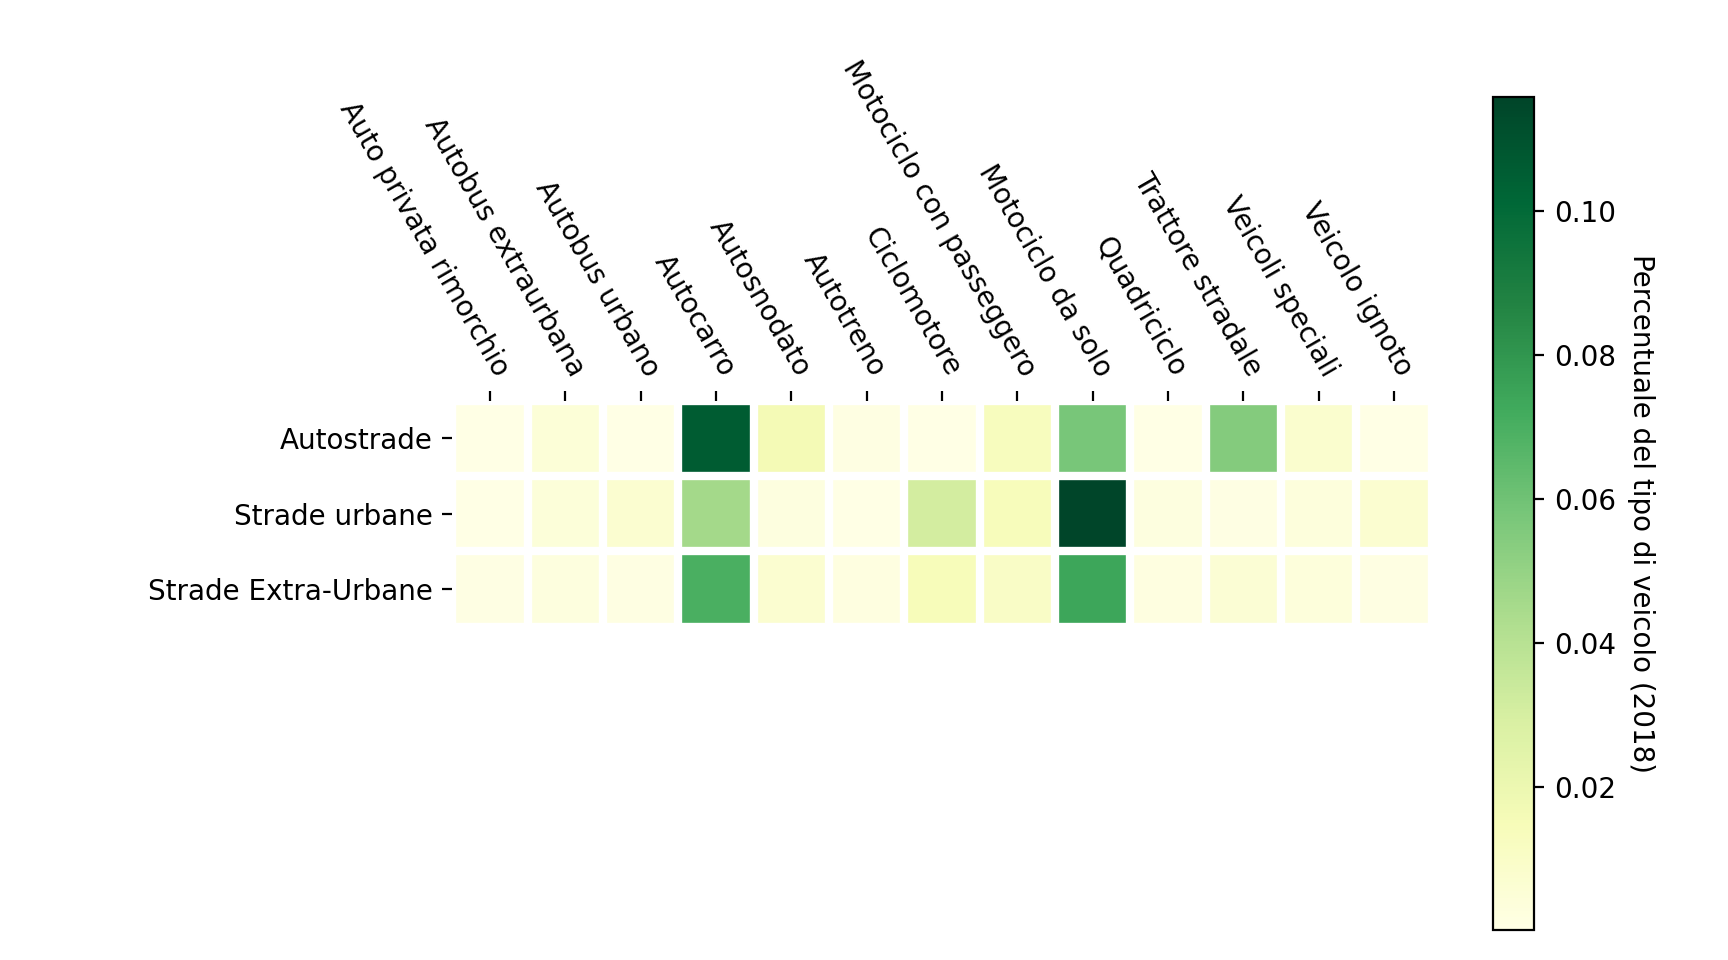
\includegraphics[width=\linewidth]{../src/incidenti/incidenti_senza_coords/tipo_veicoli/differenza_senza_auto.png}
    \caption{Incidenti per tipo veicolo, senza contare le auto private}
    \label{fig:differenza-strade-no-auto}
\end{figure}

Omesse le automobili private, appare chiaro che gli autocarri siano coinvolti in un maggior 
numero di incidenti su autostrade, mentre i motocicli abbiano il primato sulle strade urbane. 
Può anche sembrare strano che i trattori stradali siano coinvolti così spesso in incidenti 
su autostrade, tuttavia, in questo caso, per \quotestyle{trattore} non si intende la macchina 
agricola, ma la motrice di un autocarro senza rimorchio. 

Va comunque sottolineato che le percentuali di incidenti provocati da queste tipologie di 
veicoli, sono tutte al di sotto del $10$ \%, e che la sezione maggiore di sinistri è 
provocata dalle auto private. 
Inoltre, utilizzare il numero di incidenti come 
stimatore\footnote{Stimatore: una qualunque statistica con 
lo scopo di dare una stima di un parametro $\theta$ è detta stimatore 
di $\theta$ (fonte: \citetitle{PROB_E_STATISTICA:1}\cite{PROB_E_STATISTICA:1}, 
capitolo: Statistica descrittiva, pagine: 246-248)} del traffico, potrebbe non risultare 
estremamente preciso, per la presenza di fattori, come la conformazione della strada, che 
influiscono sui sinistri. 

%\clearpage
\section{Dati Istat su conducenti e passeggeri}

%\clearpage
\subsection{Esistono differenze tra la guida di un uomo e quella di una donna?}
\todo{ATOK}

% https://media.cdn.facile.it/facile/comunicati/pdf/195/original.pdf?v=20200911094353&

Un frequente stereotipo riguardante le donne, è la credenza che queste  
sarebbero meno abili alla guida rispetto alla controparte maschile. 
\todo{atrent: frase pericolosa, andrebbe sostanziata, anche se lo dici solo per poi negarla
lelepado: la ho cambiata, può andare?}
Avendo a disposizione le informazioni sul genere del conducente che ha causato l'incidente, 
è possibile controllare se esista un riscontro reale per questa credenza. 

\begin{figure}
    \hfill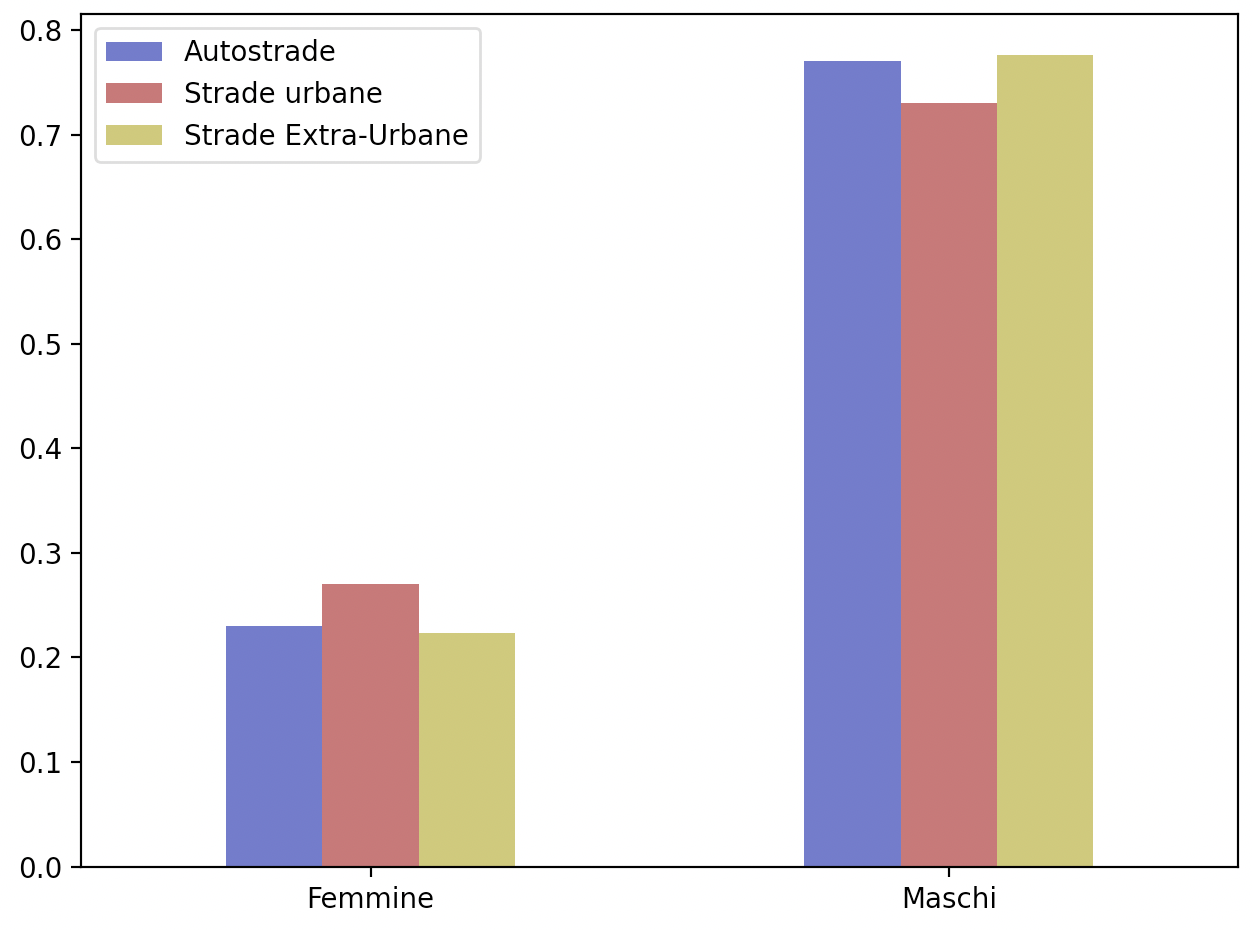
\includegraphics[width=0.7\linewidth]{../src/incidenti/incidenti_senza_coords/tipo_veicoli/uomo-donna.png}\hspace*{\fill}
    \caption{Numero di conducenti per tipo di veicolo divisi per uomini e donne nel 2018}
    \label{fig:differenza-uomo-donna}
\end{figure}

L'istogramma in figura \ref{fig:differenza-uomo-donna} mostra con quale frequenza 
gli incidenti sono causati da uomini e da donne, per tre diverse tipologie di strada. 

Per quanto riguarda la localizzazione, non è possibile individuare alcuna 
variazione nella percentuale di sinistri. 
La differenza maggiore si registra sulle strade urbane, dove le donne causano circa il 
$5$ \% di incidenti in più, nonostante ciò 
questi tendono ad essere causati per il $75$ \% circa da uomini e 
per il $25$ \% donne. 

Avendo a disposizione i dati corrispondenti a tutti gli anni a partire dal 2010, 
è anche possibile verificare che le percentuali trovate siano costanti  
nel tempo. 
Nella tabella sottostante sono riportati gli esiti dell calcolo precedente per le 
autostrade e le strade urbane. 

\begin{center}
    \def\arraystretch{1.5}% 
    \begin{tabular}{ |c|c|c|c| }
        \hline
        Anno & Sesso & Autostrade & Strade Urbane \\ 
        \hline
        \rowcolor{TableGray}
        2018 & Uomo & 77 \%  & 73 \% \\
        2018 & Donna & 23 \% & 27 \% \\
        \rowcolor{TableGray}
        2016 & Uomo & 75.8 \%  & 71.9 \% \\
        2016 & Donna & 24.2 \% & 28.1 \% \\
        \rowcolor{TableGray}
        2014 & Uomo & 74.2 \%  & 70.7 \% \\
        2014 & Donna & 25.8 \% & 29.3 \% \\
        \hline
    \end{tabular}
\end{center}

In tutti gli anni controllati, la frequenza di femmine e maschi coinvolti 
in incidenti è costante. 
Questo fenomeno, più che indicare a una mancanza di attenzione da parte degli uomini, 
fa sospettare che ci siano più persone del primo gruppo al volante rispetto al secondo. 

Un modo per confutare l'ipotesi è quello di ricavare un campione di conducenti, 
distinguendo tra uomini e donne. 
Va sottolineato che un campione, preso durante un mese prossimo alla quarantena per 
la pandemia dovuta al Covid-19, non sarà mai uno stimatore estremamente 
accurato della percentuale di maschi e femmine alla guida. 

Si sono comunque contate le persone al volante nell vetture passanti a Somma 
Lombardo\footnote{sul Sempione basso, strada urbana principale, 
nei pressi della chiesa di San Bernardino}, 
tra le 15:00 e le 16:00 di Giovedì 5 Novembre 
(settimana predente alla seconda quarantena della regione Lombardia), 
sono stati ottenuti i seguenti risultati:

\begin{center}
    \def\arraystretch{1.5}% 
    \begin{tabular}{ |c|c|c| }
        \hline
        Sesso & Numero & Percentuale \\ 
        \hline
        \rowcolor{TableGray}
        Uomini & 483 & 68.8 \% \\
        Donne & 219 & 31.2 \% \\
        \hline
    \end{tabular}
\end{center}

La percentuale di uomini e donne al volante è equivalente a quella degli incidenti. 
Si rafforza, pertanto, l'ipotesi che non esistano differenze sostanziale tra la qualità 
della guida tra i due sessi, in quanto, assumendo che la probabilità che una donna causi un 
sinistro sia uguale a quella di un uomo, i risultati ottenuti sarebbero 
gli stessi osservabili nel campione. 

\todo{atrent: potresti trovare bibliografia a supporto delle tue conclusioni, 
anche solo il fatto che le assicurazioni fanno pagare meno alle donne (almeno così sapevo) 
lelepado: ho trovato un articolo del corriere, citato sotto}
A smentire ulteriormente lo stereotipo illustrato all'inizio di questo capitolo, sono 
anche le compagnie di assicurazione di automobili che, fino al 2011, offrivano 
alle donne polizze meno costose. 
Dal mese di Dicembre 2011, questa pratica non è più stata possibile, per una direttiva della 
Corte di giustizia europea, che non permette più differenze nel prezzo della Rc auto basate 
sul sesso del conducente \cite{CORRIERE:1}, che precedentemente riducevano circa il 
18 \% di queste spese al gentil sesso, ritenuto più cauto alla guida. 

%\clearpage
\subsection{Il numero di passeggeri presenti nella vettura influisce sulla probabilità di commettere un incidente?}
\todo{ATOK}

Il dataset Istat dispone anche di una serie di colonne corrispondenti all'età, sesso 
e alla presenza di altri passeggeri a bordo del veicolo.
Analizzando i dati è possibile valutare se esiste una 
relazione tra la presenza di uno o più passeggeri e la probabilità 
di essere causa di incidente.

\begin{figure}
    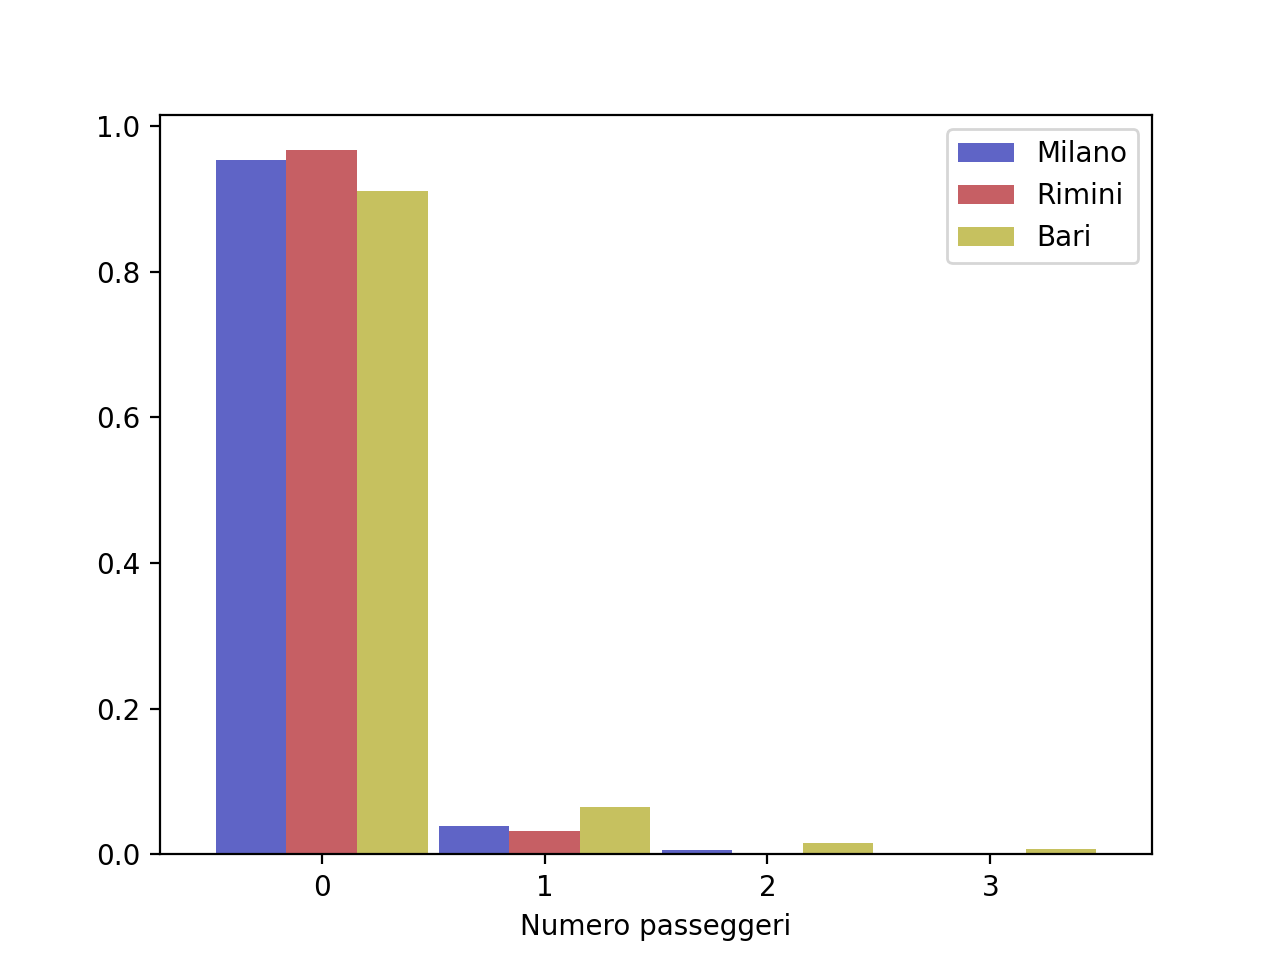
\includegraphics[width=\linewidth]{../src/incidenti/incidenti_senza_coords/passeggeri/passeggeri.png}
    \caption{Numero di passeggeri in incidenti per Milano, Rimini e Bari}
    \label{fig:passeggeri-milano-rimini}
\end{figure}

La figura \ref{fig:passeggeri-milano-rimini} mostra che oltre il $90$ \% degli eventi
avviene quando nel veicolo è presente solo il conducente, 
cioè la colonna indicata con 0. 
Si sono prese in considerazione le provincie di Milano, Rimini e Bari, 
per verificare se la località marittima influisca sul numero di incidenti. 
Non sembra però, esserci grande differenza tra le province, nonostante a Rimini sia 
più alta la categoria con solo il conducente, mentre a Bari valga l'opposto. 

Appurato, quindi, che la frequenza degli incidenti è massima in caso di guidatore solo, 
è possibile chiedersi se ciò sia dovuto a un semplice motivo quantitativo o 
se invece esistano fattori esterni che inducano alla distrazione, o 
addirittura se la presenza di passeggeri generi maggior 
attenzione per senso di responsabilità.

A tale scopo, sarebbe utile poter ricavare un campione di vetture divise per 
numero di persone a bordo, tuttavia, per il periodo in cui si è eseguito questo 
studio, la quarantena per il Covid-19 rende una stima di questo tipo 
imprecisa, in quanto la maggior parte delle persone si spostano da sole 
per viaggi di prima necessità. 

Una seconda possibilità è cercare una qualche stima del numero medio di 
persone a bordo di automobili, in una delle annate con dati su incidenti disponibili. 

Nel 2010, in un articolo per la campagna 
Sbilanciamoci!\footnote{https://sbilanciamoci.info/chi-siamo/}, 
Anna Donati scriveva: 

\begin{quotation}
    \dots infatti l’auto passa dal $59.3$ \% degli spostamenti nel 2000 al $65.3$ \% del 
    2009 e di questi ben il $57.7$ \% viaggia solo \cite{SBILANCIAMOCI:1}. 
\end{quotation}

La fonte dell'articolo è il sito Isfort\footnote{https://www.isfort.it/}, 
in particolare il loro rapporto sulla mobilità. 
Cercando nel loro archivio, non si è riusciti a reperire il rapporto del 2010, 
tuttavia si sono trovati quelli più recenti, in particolare per 
2018\footnote{\url{https://www.isfort.it/wp-content/uploads/2019/09/Rapporto_Mobilita_2018.pdf}}, 
2019, 2020. 

\`E possibile dunque ipotizzare che la percentuale di conducenti che viaggiano 
da soli, sia approssimativamente attorno al $60$ \%, perlomeno nel 2010. 
Per realizzare una stima, è necessario conoscere la quantità di automobili con uno, 
due o tre passeggeri, non presenti nell'articolo. 
Ipotizzando però, che il numero di automobili con solo conducente rimanga attorno al 
$60$ \%, è probabile che esista qualche fattore che faccia aumentare le percentuali 
degli incidenti senza passeggeri al 
$95.3$ \% visibile nel grafico \ref{fig:passeggeri-milano-rimini}. 

Uno dei fattori che si può ipotizzare, potrebbe 
essere l'utilizzo del cellulare durante la guida. 

%\clearpage
\subsection{L'aumento di utilizzo del telefono cellulare ha influenzato il numero di incidenti commessi?}
\todo{ATOK}

Non è un segreto che il numero di conducenti 
che utilizzano lo smartphone alla guida 
sia cresciuto negli anni, parallelamente all'aumento di popolarità di quest'ultimo. 

Per il giornale online l'Automobile \cite{AUTOMOBILE:1}, gli automobilisti americani 
passano quasi due minuti guardando il cellulare, in un'ora di guida. 
Questo comportamento non può che diminuire l'attenzione al volante, e di conseguenza 
aumentare la frequenza di incidenti. 
Sarebbe interessante riuscire a osservare questa tendenza con le 
informazioni a disposizione. 

Per quanto non siano disponibili dati aggiornati su questo ambito, si potrebbe confrontare gli 
anni tra 2010 e 2013, in cui l'uso del cellulare in macchina non era ancora diffuso, 
rispetto agli anni più recenti, quando gli smartphone hanno iniziato a essere utilizzati 
frequentemente durante la guida. 

\begin{figure}
    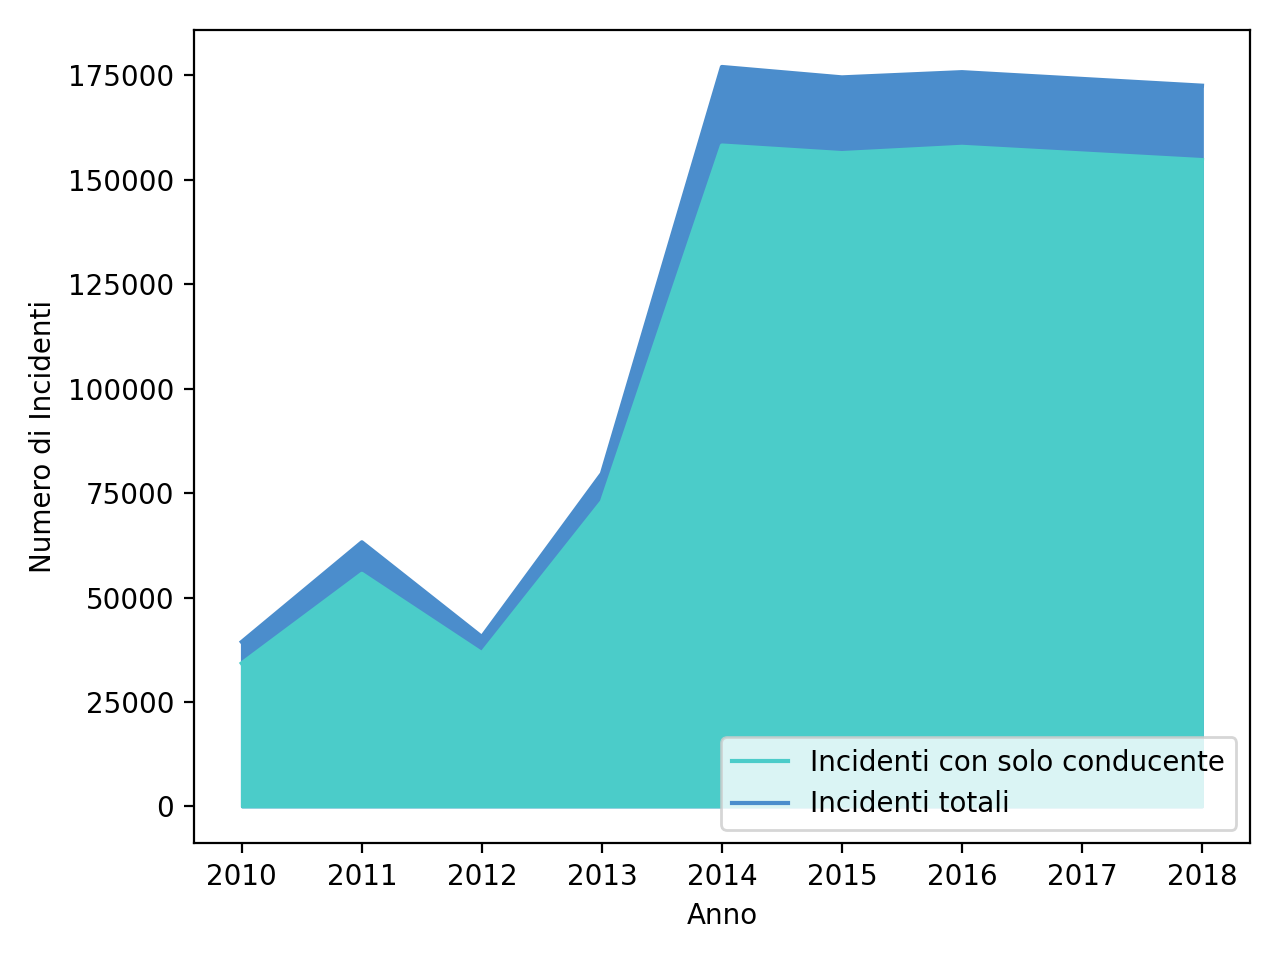
\includegraphics[width=\linewidth]{../src/incidenti/incidenti_senza_coords/anno/incremento_incidenti.png}
    \caption{Numero di incidenti all'anno, in cui è presente solo il conducente}
    \label{fig:incremento-incidenti}
\end{figure}

Nella figura \ref{fig:incremento-incidenti} è visibile l'aumento, tra 2013 e 2014, degli 
incidenti all'anno, il che supporterebbe l'ipotesi iniziale. 
Tuttavia, il numero di sinistri nei quali è presente solo il conducente 
cresce allo stesso modo, e i quelli con più di una persona nel veicolo 
salgono in maniera ancora maggiore. 
Queste tendenze sono riscontrate nell'aumento dell'ampiezza dell'area blu, nel grafico 
\ref{fig:incremento-incidenti}, che mostra un minor numero di sinistri con solo il conducente, 
e per sottrazione, l'incremento delle altre categorie. 

L'ampia crescita di incidenti, a partire dal 2013, si arresta l'anno successivo e, 
dopo il 2015 il numero di sinistri tende addirittura a diminuire, 
il che induce a pensare che siano state apportate modifiche nella medologia 
di raccolta dati, piuttosto che al cambiamento di atteggiamento da parte degli automobilisti.

L'ipotesi del telefono cellulare come fattore di distrazione per il conducente, 
non è confermabile, perlomeno con i dati di cui si dispone. 
Va anche sottolineato che le informazioni utilizzate sono influenzate da svariati fattori, ed è 
possibile \quotestyle{ipotizzare} la prevalenza di uno di questi al di sopra degli altri, 
come si è fatto con il telefono cellulare, 
ma per confermare il collegamento sarebbero necessarie indagini sicuramente 
più dettagliate ed approfondite.

%\clearpage
\section{Dati Istat su orari e mesi}

%\clearpage
\subsection{Differenze nel numero di incidenti in diversi orari della giornata}
\todo{ATOK}

Se si volesse stimare la distribuzione di traffico per fasce orarie, 
sicuramente una prima ipotesi 
deve essere quella di una curva che si alza durante il giorno, con 
punto di minimo durante la notte. 

Il risultato atteso, inoltre, potrebbe essere 
quello di osservare due picchi più o meno marcati 
in corrispondenza delle fasce orarie di entrata e di uscita dal lavoro. 
Analizzando i dati riferiti ai sinistri e non al traffico, si può, 
quindi, tentare di verificare tale ipotesi.

\begin{figure}
    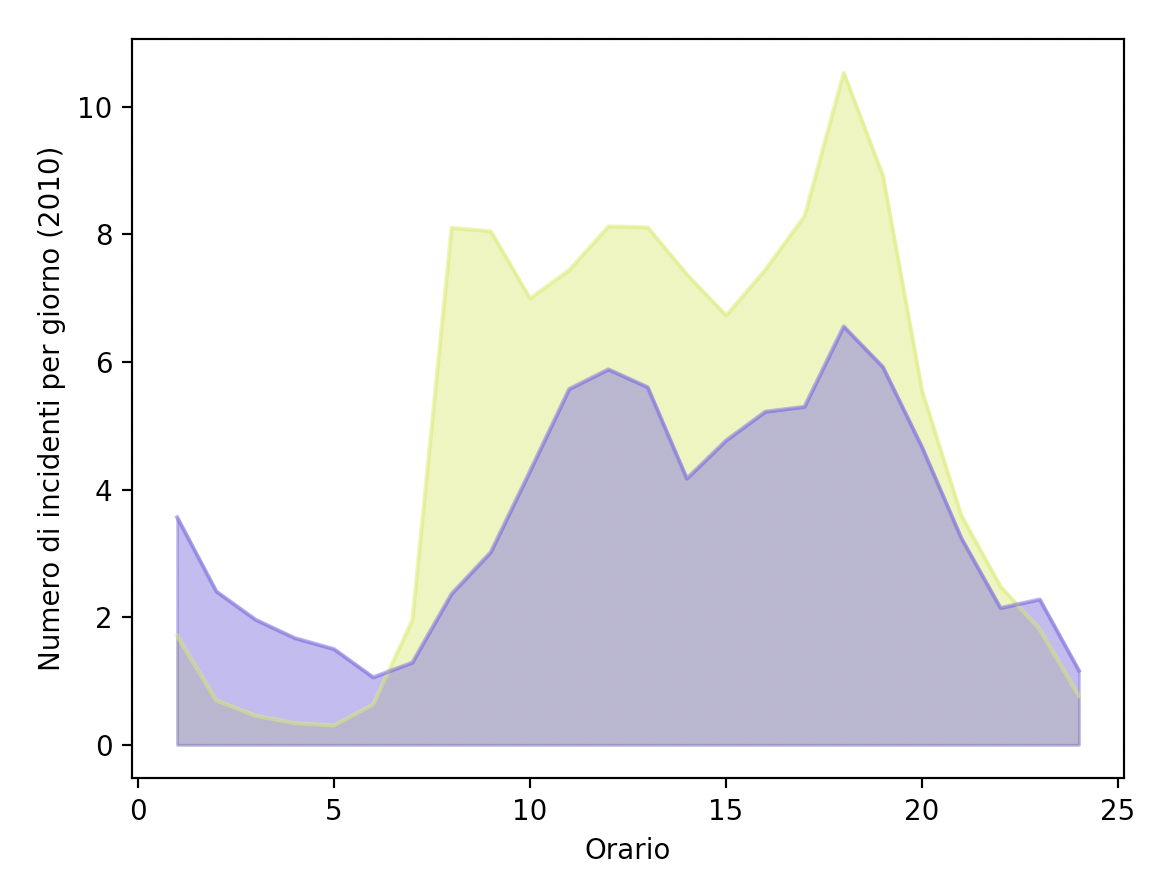
\includegraphics[width=\linewidth]{../src/incidenti/incidenti_senza_coords/ore_punta/week_weekend.png}
    \caption{Incidenti per ora}
    \label{fig:week-weekend}
\end{figure}

Tramite un semplice conteggio degli incidenti durante il weekend, e 
confrontandolo con il numero di quelli avvenuti durante la 
settimana lavorativa, si osserva come i sinistri che interessano la fascia serale 
e notturna, avvengono durante il fine settimana, quelli invece che sono commessi 
in fascia diurna sono prevalenti nelle giornate feriali. 

Per quanto riguarda, le fasce orarie \quotestyle{di punta} di cui si 
è parlato precedentemente, 
sono stati presi in considerazione, per la mattina, gli orari dalle 7:00 alle 10:00, 
e per il pomeriggio, dalle 17:00 alle 19:00. 

L'incremento durante la fascia oraria pomeridiana, presente nella figura 
\ref{fig:week-weekend}, mostra un aumento della percentuale di incidenti 
del $95.2$ \% rispetto alla media, durante la settimana lavorativa. 
Durante il weekend, si osserva comunque un incremento, ma solamente del $61.1$ \%. 

Per le fasce orarie della mattina, è comunque presente una crescita di sinistri, 
ma questo ammonta al $34.6$ \% alle 8:00, e al $80.6$ \% alle 9:00, 
mentre nel weekend si hanno addirittura percentuali di decremento 
in entrambi gli orari, rispettivamente $47.6$ \% e $17.9$ \%. 

I grafici presentati indicano i sinistri all'anno, normalizzati per numero di 
giorni settimanali o feriali, quindi gli incidenti totali della settimana sono divisi 
per cinque giorni, mentre quelli del weekend per due, 
come mostrato nel codice sottostante. 

\begin{code}[language=Python]
ora_weekend = data[data['giorno'] > 5]['Ora'].value_counts().sort_index()
ora_week = data[data['giorno'] < 6]['Ora'].value_counts().sort_index()

ora_week /= 5 * 52
ora_weekend /= 2 * 52
\end{code}

Le informazioni ricavate ricalcano in modo particolarmente preciso, 
soprattutto nelle ore del pomeriggio, le ipotesi iniziali. 

%\clearpage
\subsection{Differenze nel numero di incidenti nelle fasce orarie della mattina}
\todo{ATOK}

I risultati ottenuti nella sezione precedente sembrano indicare 
che la maggior parte degli incidenti si verifica attorno alle 9:00 di mattina. 

Questa tendenza è vera anche nel caso in cui si isoli una città come Milano, 
destinazione di molti pendolari della regione, probabilmente 
già in viaggio prima delle 9:00?

Selezionando solo i sinistri nella provincia di Milano, mostrati nel grafico 
\ref{fig:week-weekend-milano}, è possibile individuare in modo più preciso
il primo picco di incidenti, quello durante le ore di punta mattutine. 
In particolare si ha un incremento del $34.3$ \% alle 8:00 rispetto alla media, 
che aumenta fino al $118.7$ \% delle 9:00, nelle giornate lavorative. 

D'altro canto, durante il weekend, il numero di incidenti alle 8:00 cala del $58.5$ \% rispetto 
alla media e allo stesso modo alle 9:00, del $37$ \%. 

\begin{figure}
    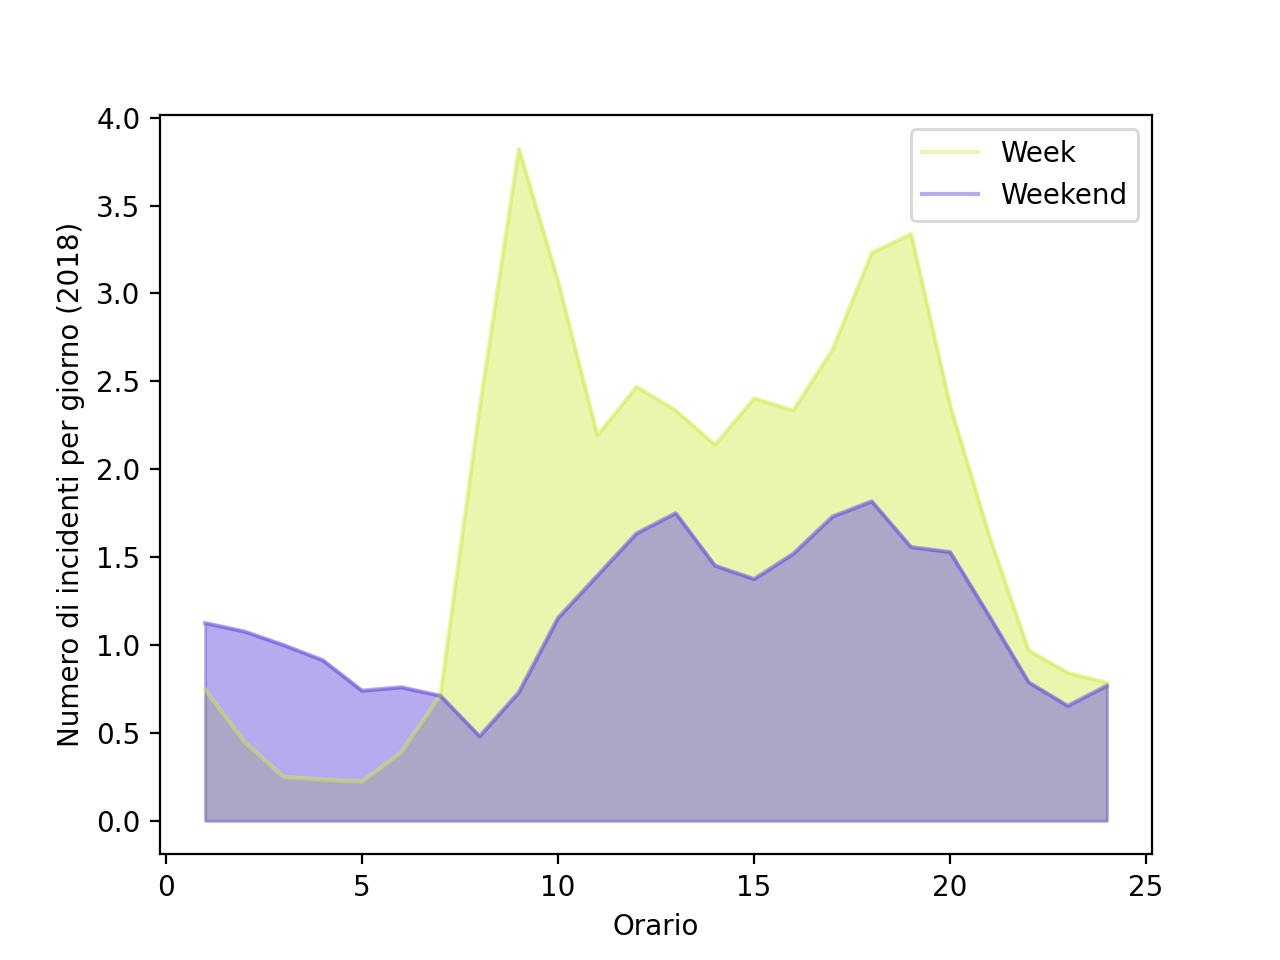
\includegraphics[width=\linewidth]{../src/incidenti/incidenti_senza_coords/ore_punta/week_weekend_milano.png}
    \caption{Incidenti per ora a Milano}
    \label{fig:week-weekend-milano}
\end{figure}

A Milano, dunque, si ha un aumento percentuale di incidenti, nelle ore della mattina, 
ancora maggiore rispetto al resto d'Italia, e il flusso di pendolari, 
alla guida in orari precedenti alle 9:00, 
non sembra influenzare il volume di sinistri. 

\subsection{Correlazione tra il numero di incidenti e traffico stradale}
\todo{ATOK}

Fino a questo momento, si è parlato di incidenti senza alcun tipo di contesto, 
e in 
particolare non si è tenuto conto del numero di automobili presenti sulle strade. 
\`E chiaro che uno dei principali fattori che causa sinistri sia proprio 
la quantità di veicoli in movimento. 
Sarebbe interessante riuscire a quantificare l'impatto della mole di traffico 
sull'incidentalità, nelle diverse ore della giornata.

Un primo problema da affrontare è quello di individuare informazioni sul 
numero di vetture presenti su strada in diverse fasce orarie. 
Per quanto un dataset contenente questi dati non sia stato trovato, 
è possibile realizzare una stima di questo carattere, 
utilizzando il numero degli ingressi all'area C di Milano, 
disponibile a partire dal 2011, fino al 2016. 

\begin{figure}
    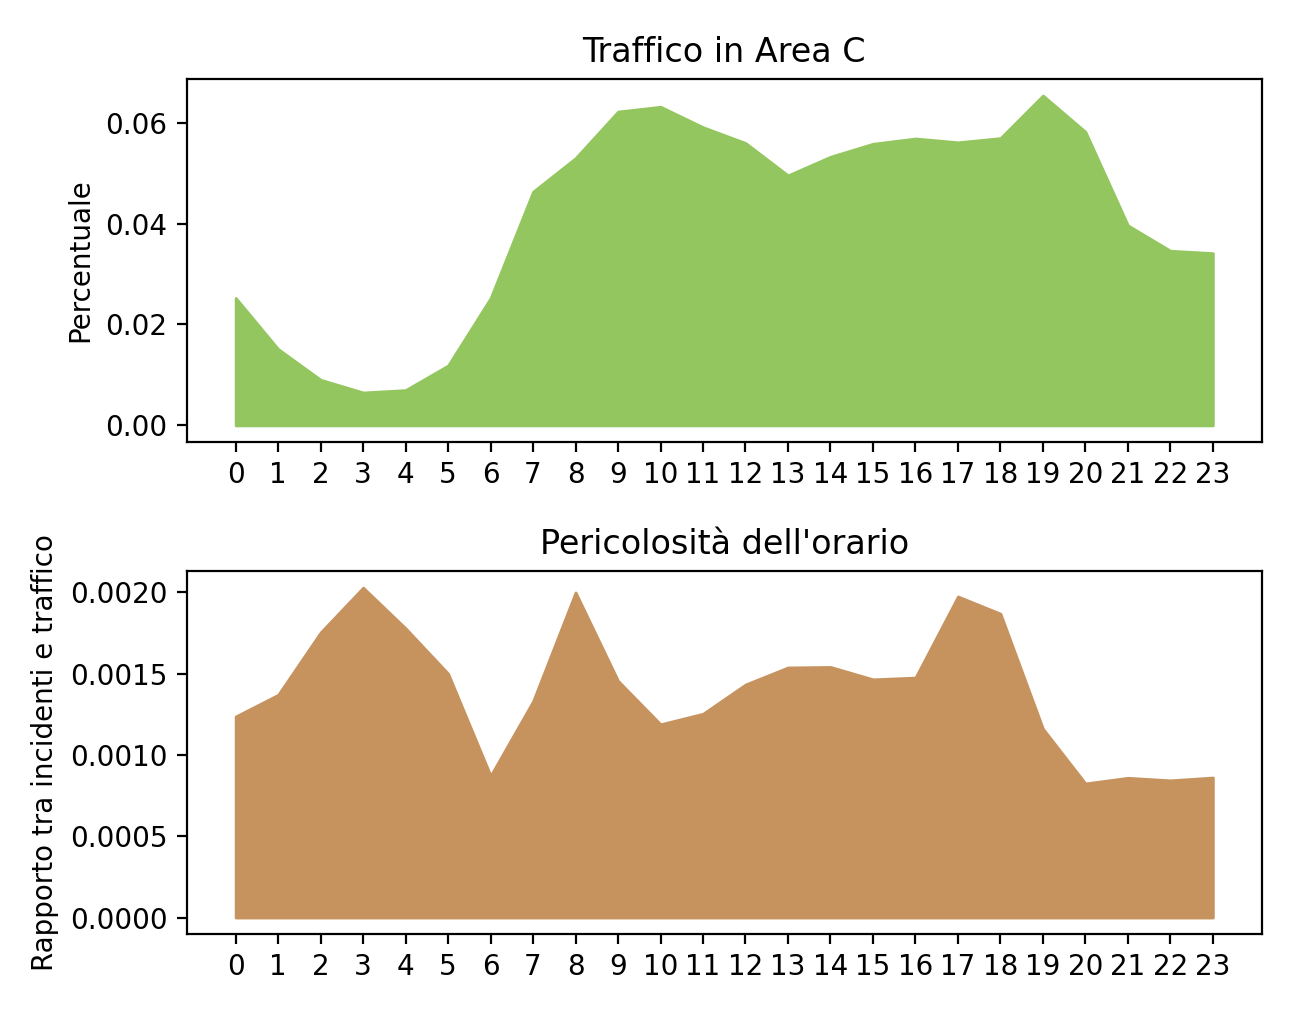
\includegraphics[width=\linewidth]{../src/area_c/rapporto_orario.png}
    \caption{Rapporto tra incidenti e traffico per orario a Milano}
    \label{fig:rapporto-incidenti-traffico}
\end{figure}

L'immagine \ref{fig:rapporto-incidenti-traffico} contiene, sulla sinistra, 
la percentuale di accessi in area a traffico limitato a una determinata 
ora\footnote{Si sono utilizzati i dati dell'anno 2016, perché non si sono trovati 
dataset più recenti per quanto riguarda gli accessi all'area C di Milano}, 
e nella figura di destra, il numero di incidenti a Milano, pesati in base alla 
stima appena realizzata. 

Sono presenti molte similitudini tra gli ingressi alla zona a traffico limitato, 
rappresentati nel grafico di sinistra nella 
figura \ref{fig:rapporto-incidenti-traffico} e l'immagine \ref{fig:week-weekend-milano}, 
raffigurante gli eventi a Milano, suddivisi per orario. 
In particolare, tra traffico in area C a Milano e 
numero incidenti, si è calcolata una correlazione pari a $0.877$. 

\begin{code}
# eseguito con dati del 2016
accessi_area_c_per_ora = pd.Series()
for f in data['hour'].unique():
    accessi_area_c_per_ora = accessi_area_c_per_ora.append(
        pd.Series(data[data['hour'] == f]['totale'].sum()), 
        ignore_index=True
        )

incidenti_per_ora = data[data['provincia'] == 15]['ora'].value_counts().sort_index()

correlazione = accessi_area_c_per_ora.corr(incidenti_per_ora)
\end{code}

Per quanto riguarda invece, il grafico sulla destra della 
figura \ref{fig:rapporto-incidenti-traffico}, sono presenti tre picchi di 
con orari particolarmente pericolosi, uno alle 3:00 di mattina, uno alle 
8:00 e l'ultimo alle 18:00. 

Di questi, il primo è possibile che sia dovuto allo scarso volume di accessi 
all'area C in questo orario, visto che alle 3:00 di notte si ha il valore minimo di 
ingressi della giornata. 

Gli altri due sono certamente dovuti all'alto 
numero di incidenti, in quanto il traffico in questi orari è pienamente nella media. 
Gli ultimi due gruppi, inoltre, corrispondono alle fasce orarie di punta, che coincidono 
con l'inizio e la fine della giornata lavorativa per la maggior parte dei milanesi. 

Chiaramente, con l'aumento del numero di automobili in viaggio, aumenta anche 
la pericolosità delle strade e la probabilità che avvenga un incidente. 

\subsection{Differenze nel numero di incidenti in orari notturni}
\todo{ATOK}

Nel grafico \ref{fig:week-weekend}, si è potuto osservare come, durante le 
ore notturne, il comportamento degli incidenti tra settimana lavorativa e weekend 
sia l'opposto, con maggior numero di sinistri durante il 
Sabato e la Domenica. 
Nell'immagine \ref{fig:ore-notte} sono raffigurati gli eventi avvenuti 
nelle principali ore della notte, divise tra settimana e weekend. 

Chiaramente, durante il fine settimana si ha un numero 
più alto di incidenti negli orari serali, 
in particolare si contano in media $5$ sinistri nelle giornate lavorative, 
mentre la quantità quasi raddoppia a $9.4$ durante il Sabato e la Domenica sera. 

\begin{code}
notte = data[(data['Ora'] < 7) | (data['Ora'] > 22)]
ora_notte_week = notte[notte['giorno'] < 6]['Ora'].value_counts().sort_index()
ora_notte_weekend = notte[notte['giorno'] > 5]['Ora'].value_counts().sort_index()

ora_notte_week /= 5 * 52  
ora_notte_weekend /= 2 * 52
\end{code}

\`E possibile ora verificare se il traffico stimato tramite il conteggio degli 
accessi in area C, dia conferma a questa tendenza.

\begin{figure}
    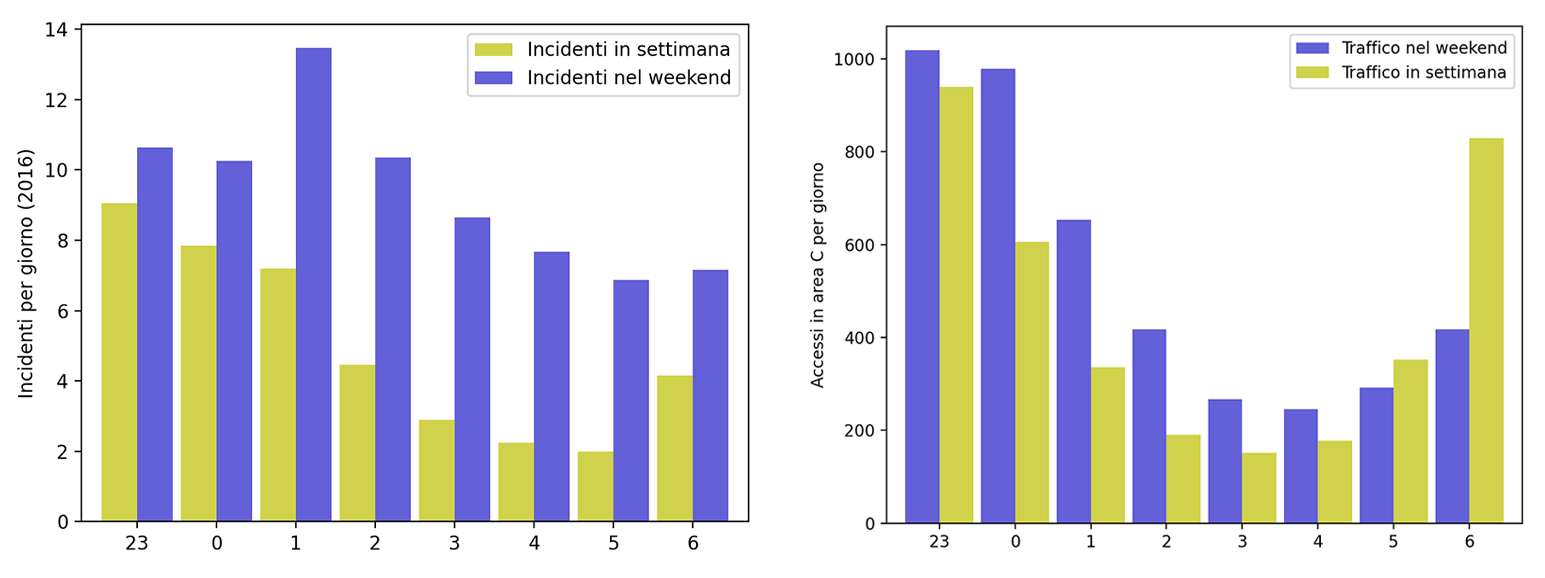
\includegraphics[width=\linewidth]{img_unite/ore_punta.png}
    \caption{Incidenti e traffico durante ore serali o notturne}
    \label{fig:ore-notte}
\end{figure}

Premettendo che la differenza di veicoli in viaggio tra settimana lavorativa e 
weekend in orari serali non è molta, il divario maggiore è presente alle ore 6:00 
in favore della settimana, mentre gli ingressi nella zona a traffico limitato 
sono maggiori nel weekend in quasi tutte le altre ore. 

Una volta ottenuti questi risultati, è possibile ricavare quali siano gli orari
più pericolosi, calcolando il rapporto tra incidenti e veicoli in movimento, 
in base all'orario. 
Il risultato è rappresentato nella figura \ref{fig:rapp-inc-traff}. 

\begin{figure}
    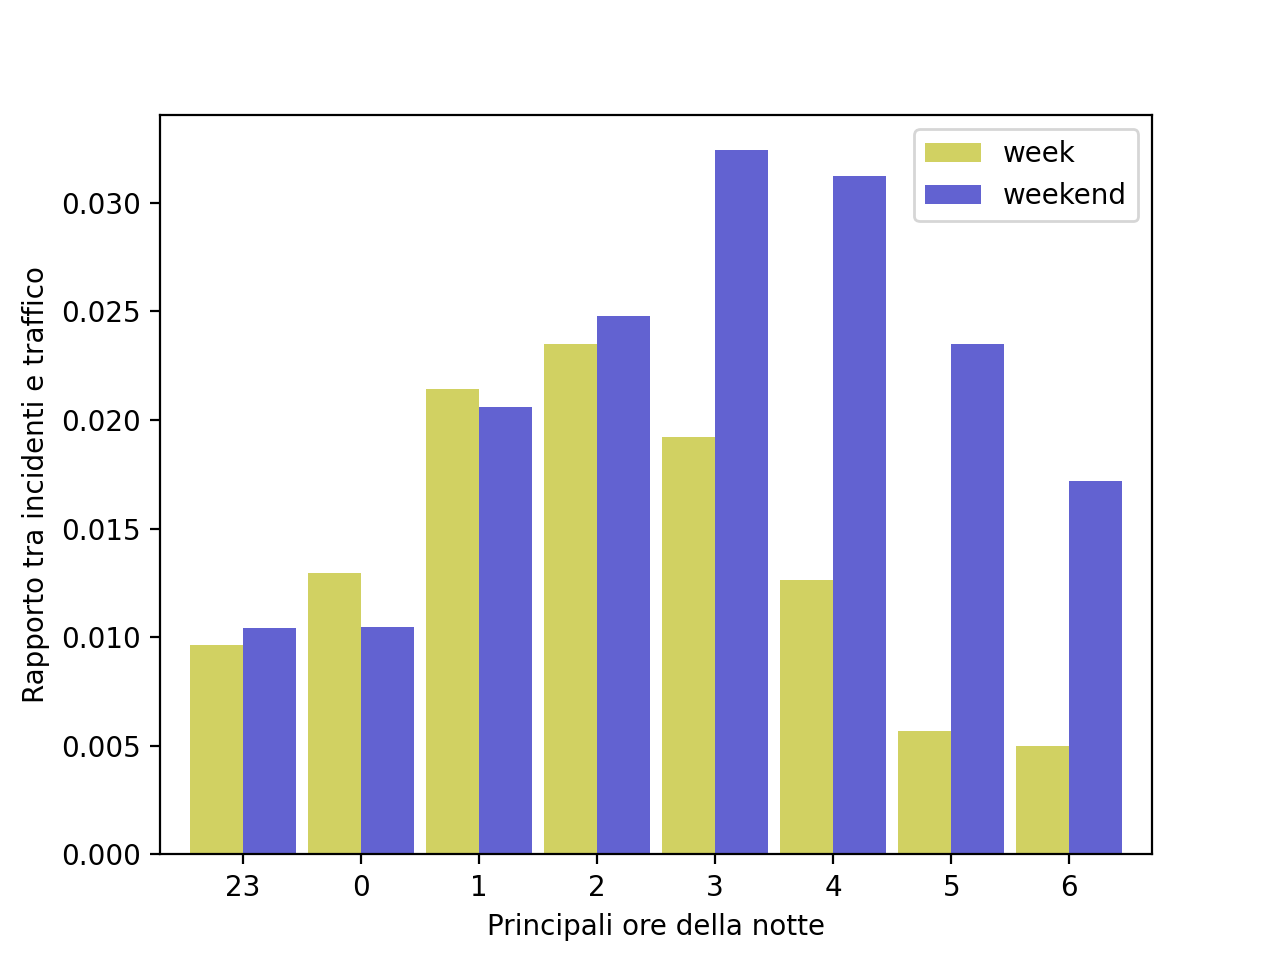
\includegraphics[width=\linewidth]{../src/area_c/rapporto_inc_notte.png}
    \caption{Rapporto tra incidenti e traffico durante ore serali o notturne}
    \label{fig:rapp-inc-traff}
\end{figure}

Durante il weekend, le ore più pericolose sono tra le 3:00 e le 4:00 di notte. 
D'altra parte, per la settimana lavorativa, gli orari con più sinistri sono quelli 
tra l'una e le tre, con un numero di incidenti rapportato al 
traffico decisamente ridotto. 

I risultati sembrano essere 
in linea, pertanto, con l'ipotesi di partenza che vedeva gli incidenti del week 
end concentrati durante le ore notturne, e viceversa in settimana i medesimi orari 
siano quelli più tranquilli.

%\clearpage
\subsection{Influenza delle vacanze sull'incidentalità nel mese di Agosto}
\todo{ATOK}

Alle analisi eseguite nei capitoli precedenti, 
è possibile aggiungere una valutazione anche riguardo i mesi più pericolosi per spostarsi, 
per una maggior probabilità di incidente.

Per fare ciò, sono necessari, non solo numeri dei sinistri avvenuti al mese, 
ma anche il dataset sugli ingressi all'area C di Milano. 
Questo è disponibile, nel caso della divisione 
mensile, fino all'anno 2018, tuttavia il campo \columnstyle{mese} nei file Istat, è 
presente solo fino all'anno 2013, ed è poi sostituito 
dalla colonna \columnstyle{trimestre}. 
Per mantenere i calcoli più precisi e attuali possibili, i grafici sull'argomento prenderanno 
in considerazione l'annata più recente contenente il label \columnstyle{mese}. 

\begin{figure}
    \hfill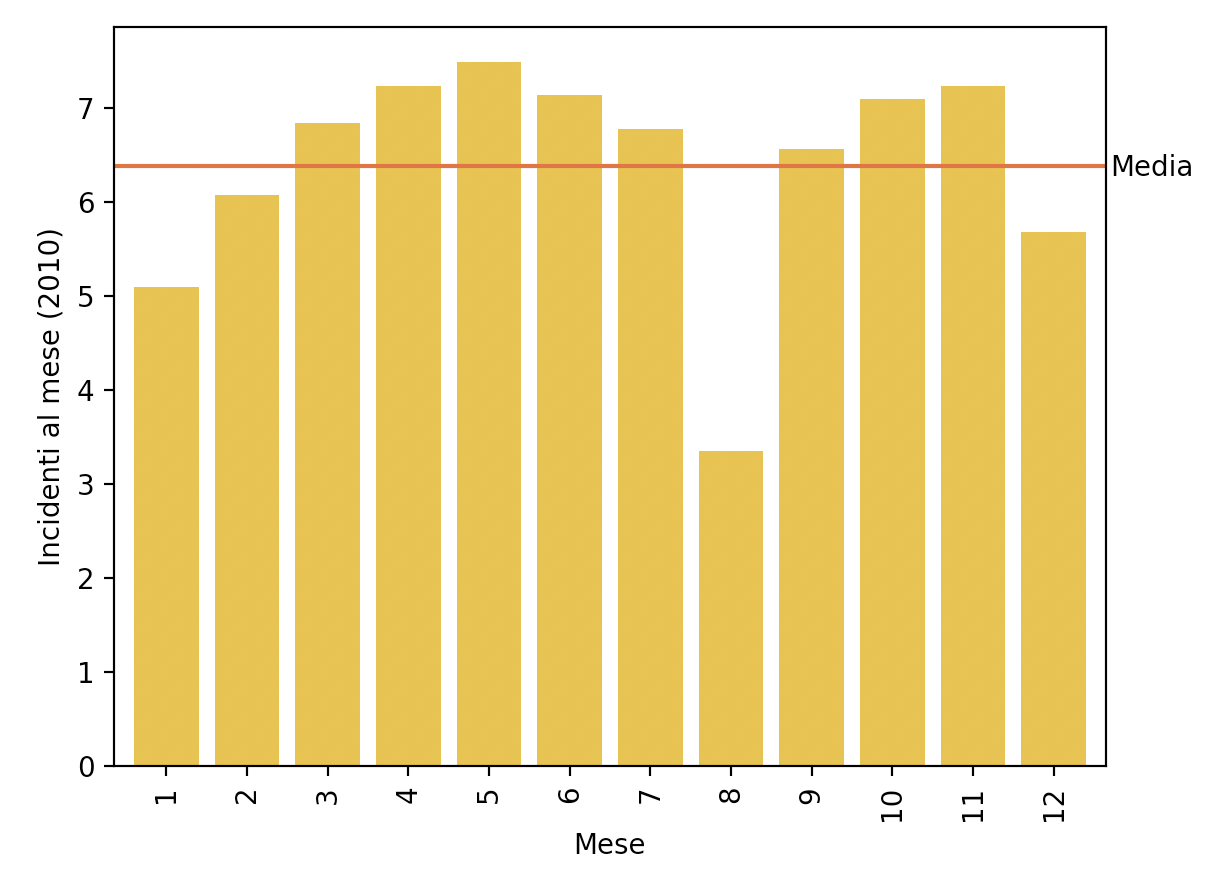
\includegraphics[width=0.7\linewidth]{../src/incidenti/incidenti_senza_coords/mese_incidenti/milano_mese.png}\hspace*{\fill}
    \caption{Incidenti per mese in Milano nel 2013}
    \label{fig:milano-mese}
\end{figure}

Nel grafico \ref{fig:milano-mese}, che rappresenta gli incidenti avvenuti a Milano ogni mese, 
si osserva una crescita di sinistri che parte dai primi periodi 
dell'anno, che termina in Luglio e cala notevolmente in Agosto. 
Per verificare che questo comportamento non sia 
un caso unico, la percentuale di decremento è riportata nella tabella sottostante, 
assieme agli altri anni per cui si ha disponibilità di dati. 

\begin{center}
    \def\arraystretch{1.5}%  
    \begin{tabular}{ |c|c| } 
        \hline
        Anno & Decremento in Agosto \\ 
        \hline
        2010 & 47.4 \%  \\ 
        \rowcolor{TableGray}
        2011 & 35.14 \% \\
        2012 & 45.46 \% \\
        \rowcolor{TableGray}
        2013 & 41.37 \% \\
        \hline
    \end{tabular}
\end{center}

Ciò che si potrebbe dedurre, in modo errato, dalla figura \ref{fig:milano-mese}, 
è l'idea che, in Agosto, ci si metta alla guida con più attenzione, 
e dunque si causino meno incidenti. 
Pur non potendo escludere a priori tale ipotesi, i fattori che determinano 
il decremento dei sinistri possono essere molteplici, 
ma certamente l'esodo verso le località di villeggiatura ha un peso marcato.

Un modo per verificare questa teoria è controllare se il traffico, 
stimato tramite i dati sugli ingressi in area C, cali durante il mese di 
Agosto a Milano. 
A supporto dell'ipotesi iniziale, nella figura sinistra \ref{fig:incidenti-traffico-mese}, 
è visibile un calo di accessi alla zona a traffico limitato, 
durante i mesi di Giugno, Luglio e Agosto. 

Una volta ottenuta una stima di questo fattore, è possibile calcolare quali mesi 
siano più pericolosi dal punto di vista degli incidenti, 
rapportando il loro numero agli ingressi in area C mensili.

\begin{figure}
    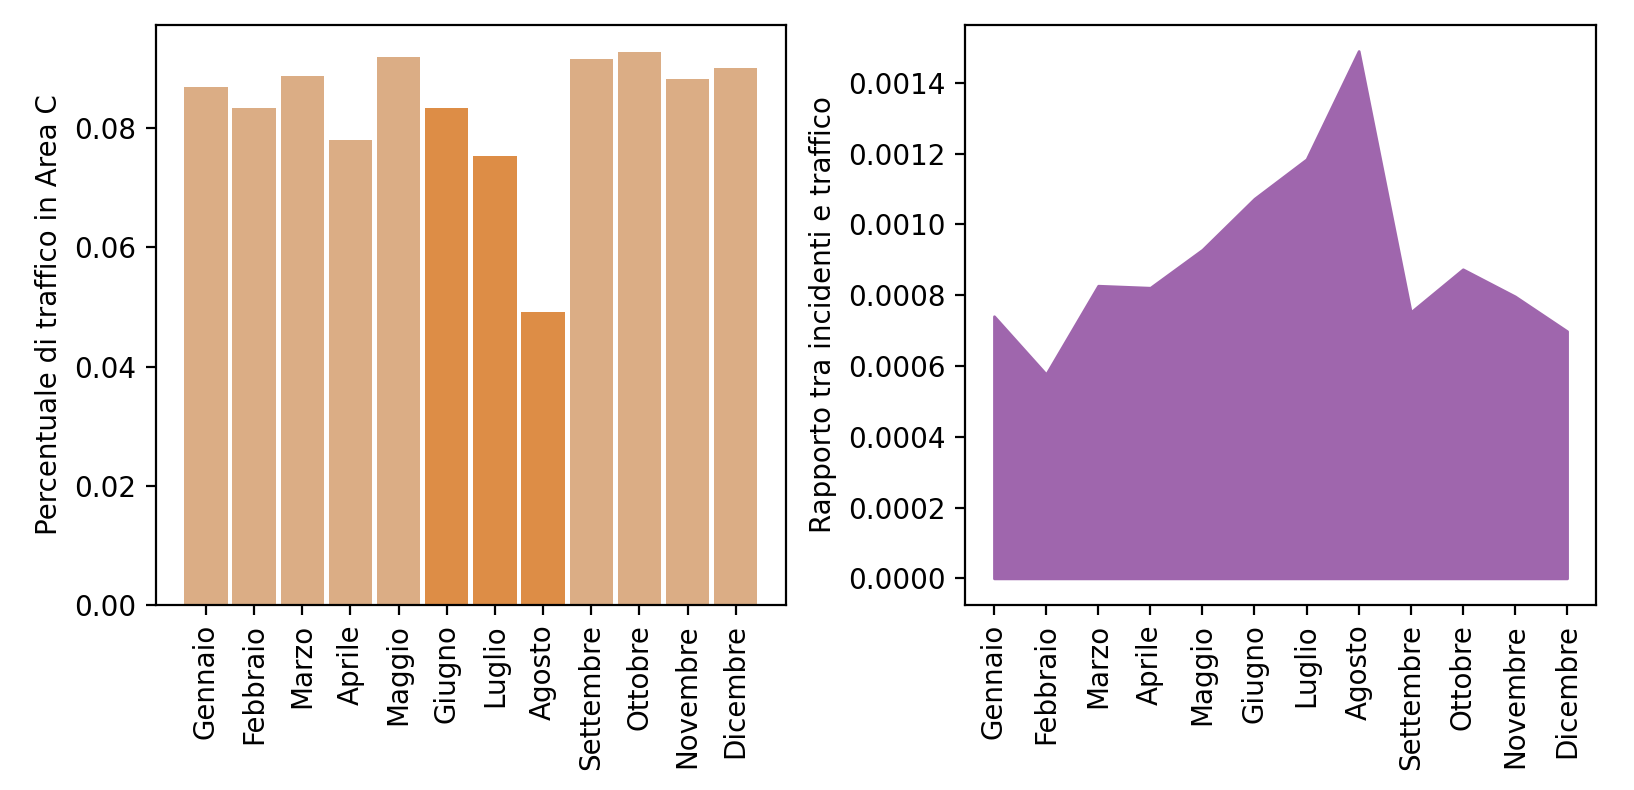
\includegraphics[width=\linewidth]{../src/area_c/rapporto_mese.png}
    \caption{Incidenti al mese, tenendo conto del traffico nello stesso periodo (2012)}
    \label{fig:incidenti-traffico-mese}
\end{figure}

L'immagine \ref{fig:incidenti-traffico-mese} contiene due grafi, 
il primo riguardante la frazione di traffico annuale che interessa ogni mese, 
mentre il secondo raffigura il rapporto tra il numero di incidenti mensili, 
e il carattere presente nel primo
istogramma\footnote{Si è utilizzato l'anno 2012 perché è il primo anno contenente 
tutti i dati completi, tutti gli altri anni hanno mesi o campi mancanti, 
per esempio il file corrispondente all'anno 
2013 non ha le misurazioni per tutto il mese di Dicembre}. 

Nel grafico di destra il valore massimo corrisponde al mese di Agosto 
che, nonostante abbia minore volume di sinistri, 
una volta tenuto conto della quantità di traffico, risulta essere 
il mese in cui si contano più incidenti. 

\skipline
A partire dal 2014, il campo \columnstyle{mese} è stato convertito nella 
colonna \columnstyle{trimestre}. 
Si potrebbe comunque eseguire un calcolo analogo a quello precedente, 
per tentare di visualizzare lo stesso fenomeno con campioni più ampi. 

La figura \ref{fig:milano-trimestri} mostra la quantità di incidenti per 
trimestre a partire dal 2010 fino al 2018. 

\begin{figure}
    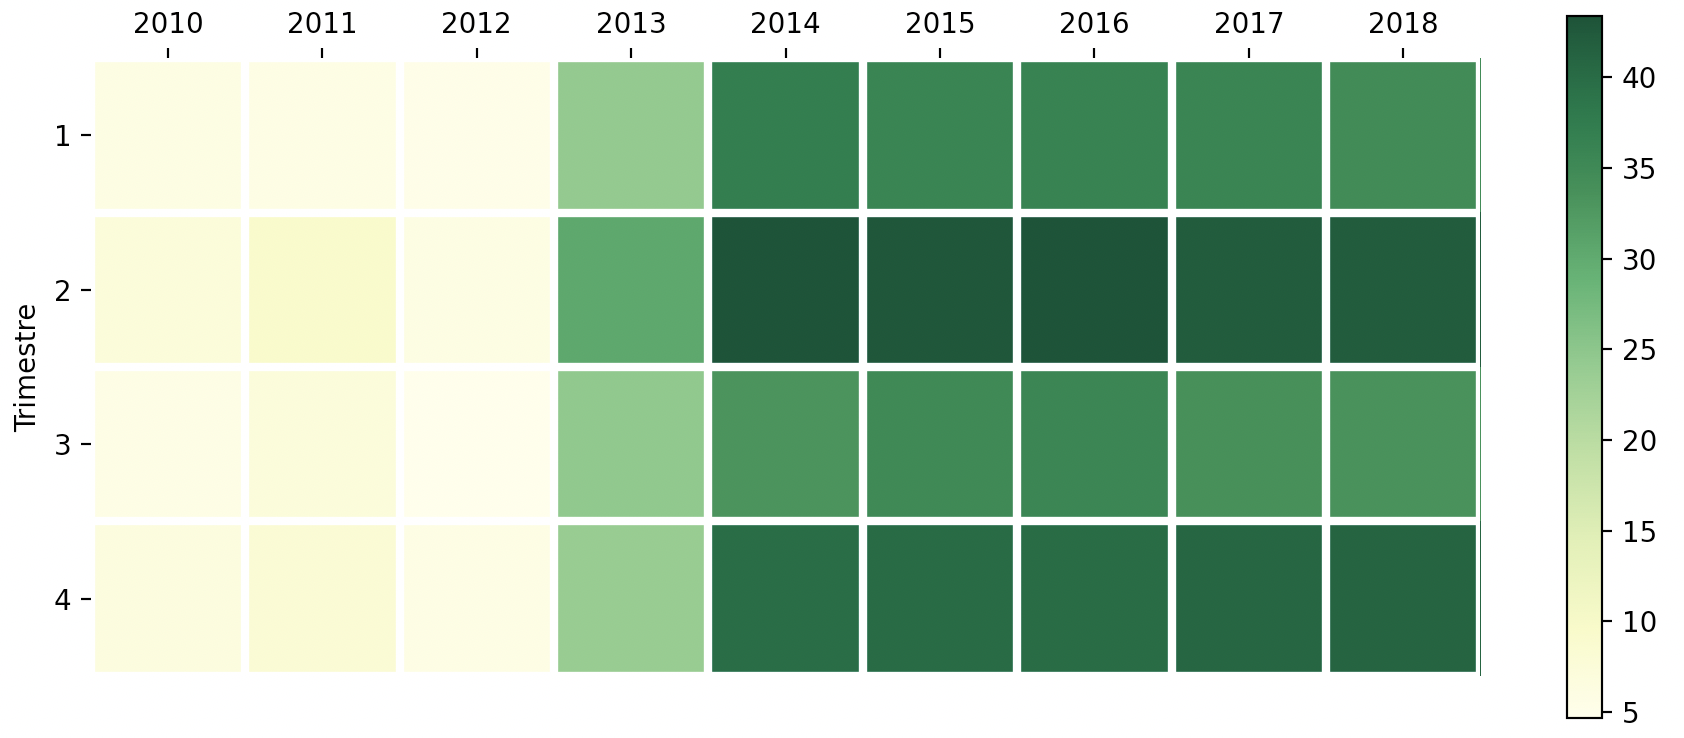
\includegraphics[width=\linewidth]{../src/incidenti/incidenti_senza_coords/mese_incidenti/trimestri.png}
    \caption{Incidenti per trimestre a Milano}
    \label{fig:milano-trimestri}
\end{figure}

Per prima cosa, va detto che è possibile osservare anche in questo grafico 
l'aumento di sinistri a partire dall'anno 2013, di cui si è parlato nel capitolo 
riguardante l'utilizzo del cellulare alla guida. 

In secondo luogo, per quanto riguarda i trimestri, è chiaro che quello estivo abbia 
un numero minore di incidenti. 
Tuttavia, in questo caso, il volume del primo periodo è comparabile 
con quello del terzo, 
mentre durante il secondo e il quarto avvengono la maggior parte dei sinistri. 

La maggiore omogeneità nei risultati calcolati in questa heatmap, 
è dovuta all'utilizzo di campioni più ampi, di novanta giorni e non di trenta, 
che permettono di bilanciare i valori fuori dalla norma, 
come quelli riscontrati per Agosto. 

\subsection{Differenze di incidenti in località di mare nei mesi estivi}
\todo{ATOK}

Osservando il grafico in figura \ref{fig:milano-mese}, 
ci si può chiedere se alla diminuzione degli incidenti estivi in città, 
corrisponda una tendenza inversa nelle località di villeggiatura.

In altre parole, visto che un gran numero di persone si sposta in automobile 
verso altre regioni durante i mesi estivi, la differenza di traffico è osservabile 
nella quantità di sinistri?

\begin{figure}
    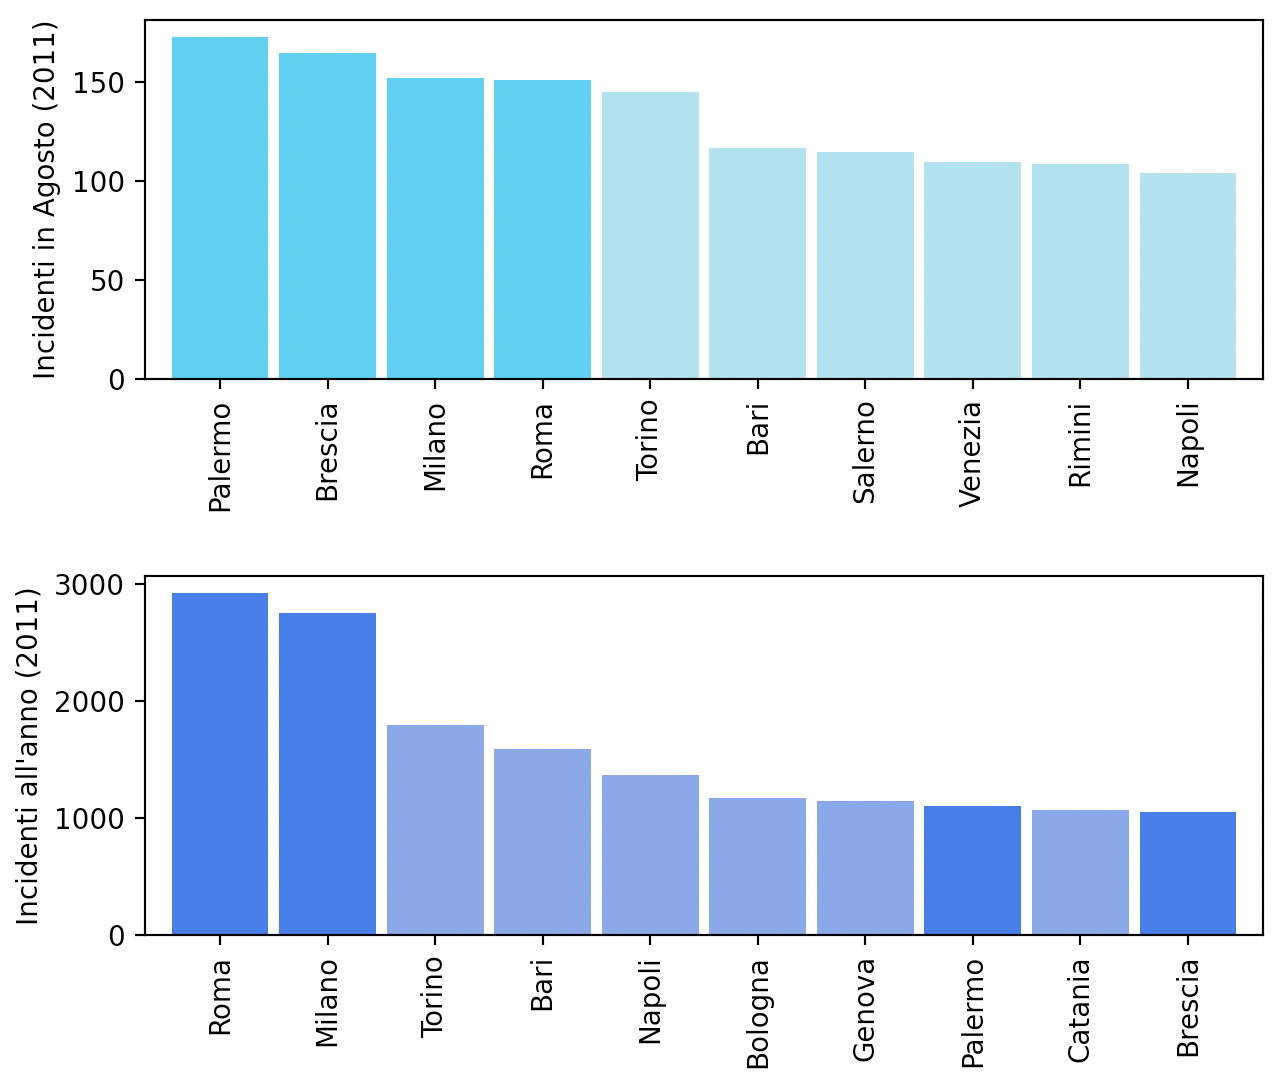
\includegraphics[width=\linewidth]{../src/incidenti/incidenti_senza_coords/mese_incidenti/mesi_estivi.png}
    \caption{Prime 10 province per incidenti in Agosto rispetto a tutto l'anno}
    \label{fig:mesi-estivi}
\end{figure}

Nella figura \ref{fig:mesi-estivi} sono elencate le province con maggiore incidentalità 
in Agosto rispetto a tutto l'anno, nel 
2011\footnote{Si è utilizzato l'anno 2011 perché mostra un comportamento diverso rispetto a 
tutte le altre annate disponibili}. 
In particolare, ad aumentare di valore sono le zone vicino a Brescia e Palermo. 

Il comportamento rappresentato nel grafico, tuttavia, è unico del 2011, in quanto, 
per gli altri anni di cui si dispone dei dati, 
Milano e Roma hanno il primato di incidenti sia per l'anno, come ci si attende, sia per il 
mese di Agosto preso singolarmente. 


D'altra parte, se si pensasse di comparare più nel dettaglio alcune province, 
meta di vacanze estive, con Milano, ciò che ci si aspetterebbe è 
di avere un incremento di sinistri in Luglio e 
Agosto\footnote{Si è utilizzato l'anno più recente per i dati a disposizione, 
a partire dal 2014 non sono più disponibili dati riguardanti il mese}. 
Per eseguire questo confronto sono state prese in considerazione le 
località di Rimini e Palermo, mostrando che alcune province, come la prima, 
confermano l'ipotesi, mentre altre, 
come la seconda, possono essere usate come controesempio. 

\begin{figure}
    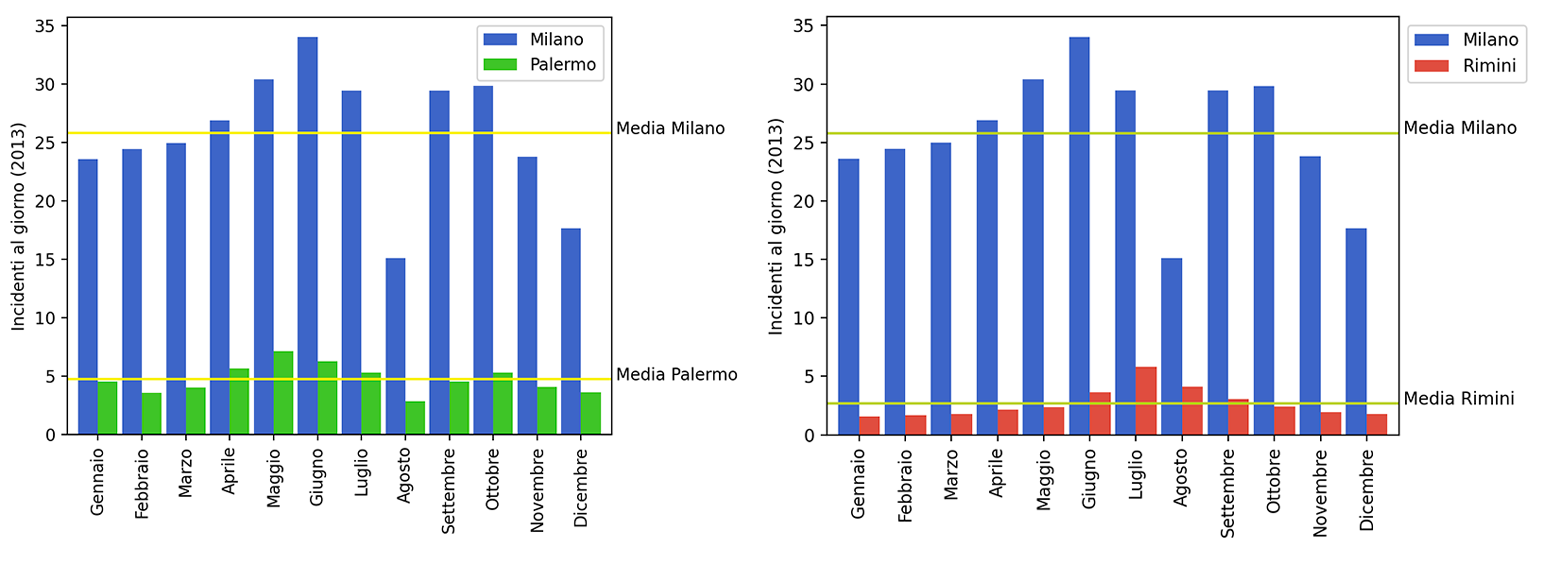
\includegraphics[width=\linewidth]{img_unite/milano_rimini_palermo.png}
    \caption{Incidenti per mese a Milano, Rimini e Palermo}
    \label{fig:milano-rimini}
\end{figure}

Il confronto tra Milano e Rimini è raffigurato nell'immagine sinistra della 
figura \ref{fig:milano-rimini} e, nonostante nella prima zona 
avvengano un numero maggiore di 
incidenti rispetto alla provincia Emiliana, nei mesi estivi, 
la quantità di sinistri a Rimini è superiore alla media annuale, 
mentre nel capoluogo lombardo è inferiore. 
Inoltre, a Milano si ha una tendenza di diminuzione in Agosto e nei 
mesi invernali, mentre a Rimini si ha incremento nei mesi estivi. 

In provincia di Palermo, visibile nell'istogramma destro in figura \ref{fig:milano-rimini}, 
d'altra parte, non risulta che nessun mese abbia un numero di incidenti 
particolarmente più alto della media, anzi, questa sembra imitare il comportamento di 
Milano, con Agosto e i mesi invernali più bassi. 

Nella seguente tabella, sono indicate le percentuali di aumento per annata dei sinistri 
a Rimini. 
L'incremento, più o meno costante in ogni anno, conferma questo fenomeno come un trend 
annuale, e non come un outlier dovuto a un 2013 fuori dalla norma. 

\begin{center}
    \def\arraystretch{1.5}%  
    \begin{tabular}{ |c|c|c| } 
    \hline
    Anno & Luglio   & Agosto \\ 
    \hline
    \rowcolor{TableGray}
    2010 & 101.72 \% & 63.75 \% \\ 
    2011 & 54.6  \%  & 60.49 \% \\
    \rowcolor{TableGray}
    2012 & 75.97 \%  & 45.93 \%\\
    2013 & 116.37 \% & 51.82 \%\\
    \hline
    \end{tabular}
\end{center}

Questo tipo di analisi può essere estesa a livello regionale, 
per esempio in Valle d'Aosta e su base stagionale, per esempio per 
comparare le vacanze invernali sugli sci. 
Nel grafico in figura \ref{fig:aosta}, si notano crescite nel numero di incidenti 
in Valle d'Aosta, nei mesi di Giugno e Settembre, tuttavia, nei periodi invernali, 
la quantità di sinistri è generalmente più bassa rispetto alla media. 

\begin{figure}
    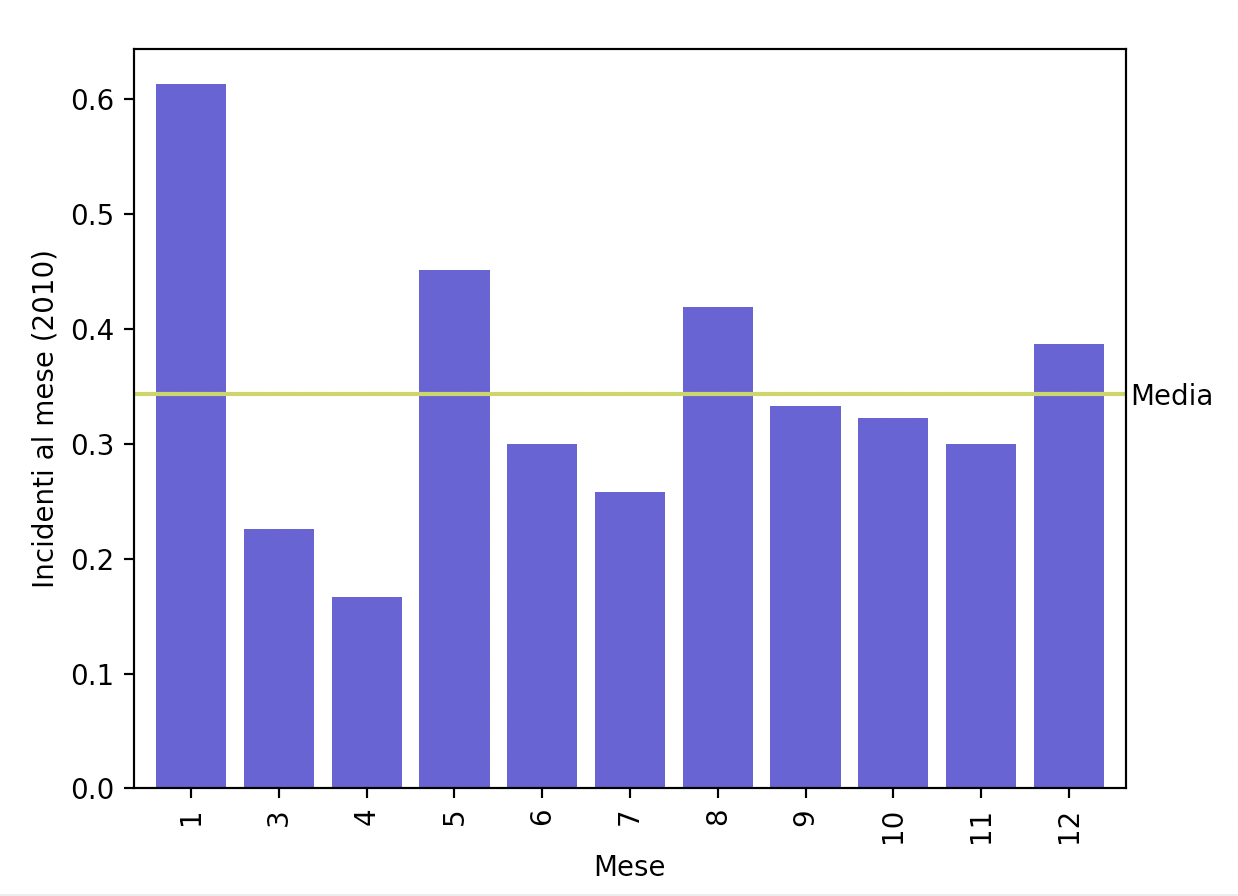
\includegraphics[width=\linewidth]{../src/incidenti/incidenti_senza_coords/mese_incidenti/aosta_mese.png}
    \caption{Incidenti per mese Valle d'Aosta}
    \label{fig:aosta}
\end{figure}

La prima cosa che è possibile controllare, è se questa tendenza venga confermata negli anni. 
Nella tabella sottostante sono stati riportati gli incrementi percentuali di incidenti 
rispetto alla media annuale, per ogni annata disponibile. 

\begin{center}
    \def\arraystretch{1.5}%  
    \begin{tabular}{ |c|c|c| } 
    \hline
    Anno & Gennaio & Agosto \\ 
    \hline
    \rowcolor{TableGray}
    2010 & 78.48 \%  & -2.93 \%\\ 
    2011 & -32.12 \% & 124.0 \%\\
    \rowcolor{TableGray}
    2012 & -41.44 \% & 52.25 \% \\
    2013 & -24.63 \% & -15.21 \% \\
    \hline
    \end{tabular}
\end{center}

Il comportamento mostrato in Valle d'Aosta, sia nella tabella, 
che nella figura \ref{fig:aosta-rimini-milano-trimestre}, non è molto costante, 
soprattutto in Agosto. 

Va specificato che la taglia del campione con cui si sta lavorando, per questa provincia, 
è molto ridotta, e sicuramente influisce sulle tendenze di incremento e decremento 
degli incidenti. 
Nonostante ciò, assumendo che Gennaio 2010 sia un outlier, il numero di sinistri in 
questo mese è sempre in diminuzione rispetto alla media, con percentuali abbastanza alte. 

L'inconsistenza registrata ad Aosta è comune anche ad altre località di montagna, come Trento e 
Bolzano, e potrebbe essere dovuta a diversi fattori, come 
le dimensioni ridotte delle città, oppure il manto stradale meno esteso, oppure ancora, 
una guida particolarmente virtuosa e attenta.

Per avere una visione di insieme delle tendenze di tutti gli anni disponibili, 
è possibile tracciare 
il grafico \ref{fig:aosta-rimini-milano-trimestre}, dividendo gli eventi 
per trimestre\footnote{Per primo trimestre si intende Gennaio, Febbraio e Marzo ecc.}. 

\begin{figure}
    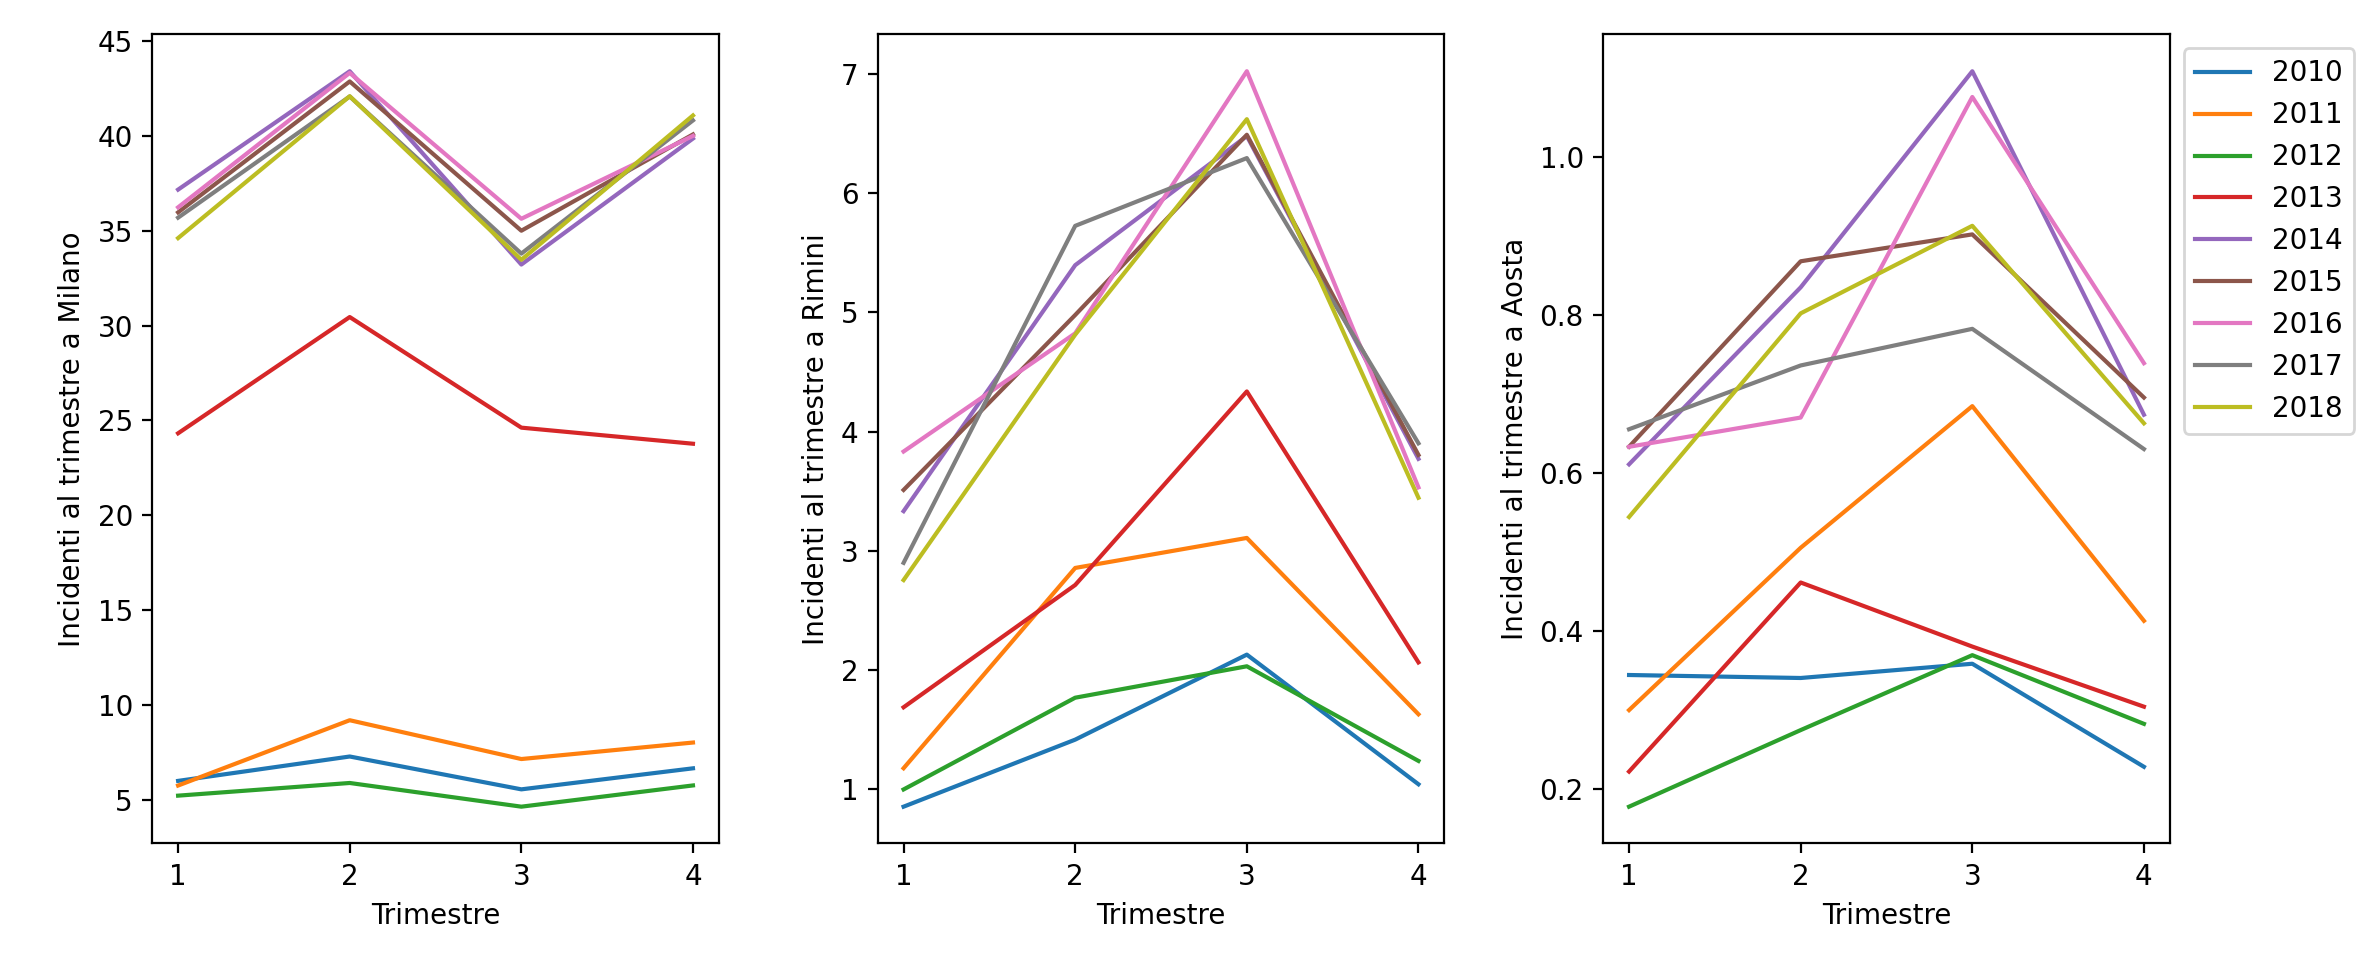
\includegraphics[width=\linewidth]{../src/incidenti/incidenti_senza_coords/mese_incidenti/trimestri_aosta_milano_rimini.png}
    \caption{Incidenti per trimestre in Valle d'Aosta, a Rimini e a Milano}
    \label{fig:aosta-rimini-milano-trimestre}
\end{figure}
\todo{atrent: attenzione alle scale!!! dovunque tu vuoi fare un confronto 
visivo tra grafici devi avere la stessa scala!!! vale dappertutto, l'ho notato qui, 
fai verifica su tutta la tesi 
lelepado: intende Aosta? i valori sono tutti assoluti, ma 
nella provincia ce ne sono così pochi che sembrano tra 0 e 1 normalizzati}

In tutti i grafici nella figura \ref{fig:aosta-rimini-milano-trimestre}, 
si osserva, come già visto in precedenza, che dall'anno 2015 si ha un'ampia crescita  
del numero di incidenti, probabilmente dovuta a un cambio 
nella metodologia di misurazione dei dati. 

Per quanto riguarda Rimini e Aosta, si osservano varie similitudini in quasi 
tutte le annate. 
In particolare, si ha un basso numero di sinistri 
durante il primo trimestre, e un incremento durante il terzo. 
D'altra parte, a Milano, è visibile la tendenza opposta, con maggior quantità di 
incidenti nel secondo periodo, e un abbassamento durante il primo 
e terzo, soprattutto con l'aumento della taglia del campione, 
a partire dal 2015. 

Ciò che è possibile dedurre, è che a Milano il numero di sinistri decresce 
nel terzo trimestre in corrispondenza con le partenze per le vacanze, mentre nelle 
altre località raffigurate, avviene il comportamento opposto poiché 
queste sono spesso mete feriali. 

Sarebbe interessante individuare l'esistenza di destinazioni di vacanza preferite, 
indipendentemente dall'anno, o se queste cambino di stagione in stagione. 
Si tenterà di rispondere a queste domande nei capitoli successivi. 

%\clearpage
\section{Dati Istat su tipi di incidenti e incroci}

Avendo a disposizione informazioni sulle località degli incidenti 
e sul tipo di incrocio, 
sarebbe interessante sapere se esistano tipologie di sinistri che accadono 
con più frequenza di altre. 

Un'altra questione potrebbe essere se, tra queste categorie, il numero di feriti 
sia comparabile o se alcuni tipi di sinistri siano più pericolosi di altri. 

%\clearpage
\subsection{Frequenza di incidenti per tipologia }
\todo{ATOK}

Per rispondere alla prima delle domande poste nell'introduzione, è possibile, 
utilizzando i dati a disposizione, contare la frequenza di ogni categoria di incidente. 

\begin{figure}
    \hfill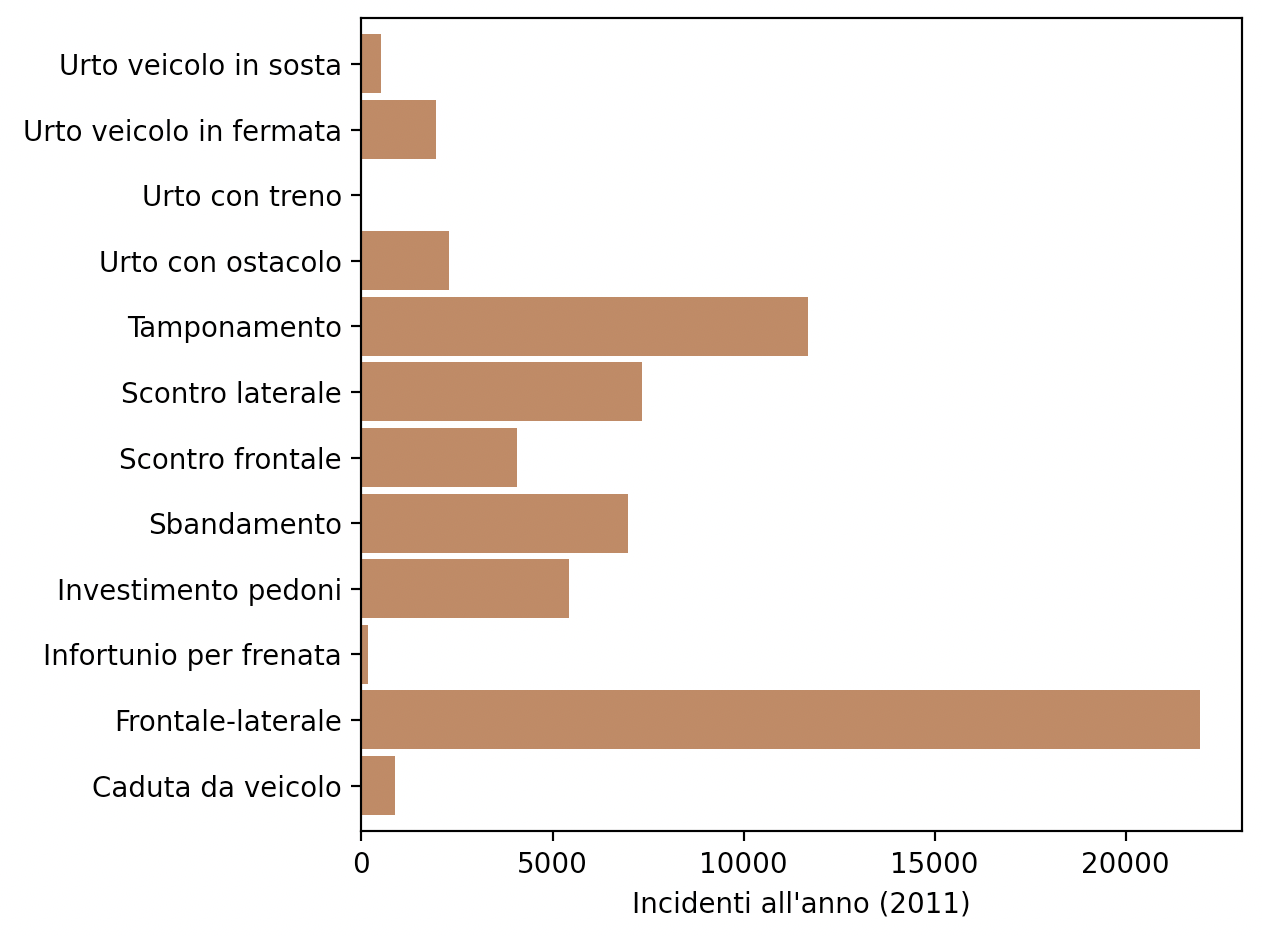
\includegraphics[width=0.7\linewidth]{../src/incidenti/incidenti_senza_coords/localizzazione_incidente/tipo_incidente.png}\hspace*{\fill}
    \caption{Numero di incidenti divisi per tipologia}
    \label{fig:tipo-incidente}
\end{figure}

Nella figura \ref{fig:tipo-incidente} sono riportate le circostanze di 
incidente più frequenti nel 2018. 
In particolare, sono molto numerosi gli scontri frontali, laterali e tamponamenti. 
La tipologia \columnstyle{frontali-laterali} è quella più rappresentata, 
probabilmente per l'ampiezza della categoria, in quanto contiene 
tutte le sfumature di incidenti che non sono 
contatti precisamente frontali o precisamente laterali. 

Prima di realizzare assunzioni errate, va detto che questo grafico, senza un contesto, 
non è molto utile, poiché il numero di incidenti di una categoria deve 
essere strettamente influenzato dalla tipo di strada e intersezione. 
Per esempio, si ha una probabilità bassa di essere coinvolti in un tamponamento 
se si sta guidando su un'autostrada, mentre il numero di casi aumenta se si viaggia 
su un viale con più semafori in serie. 

Ciò che è possibile controllare, è se negli altri anni disponibili, le 
tipologie di intersezioni rimangano costanti o meno. 
Le percentuali delle categorie di incroci che provocano più sinistri 
sono riportate nella figura \ref{fig:rapporto-tipologie}: 

\begin{figure}
    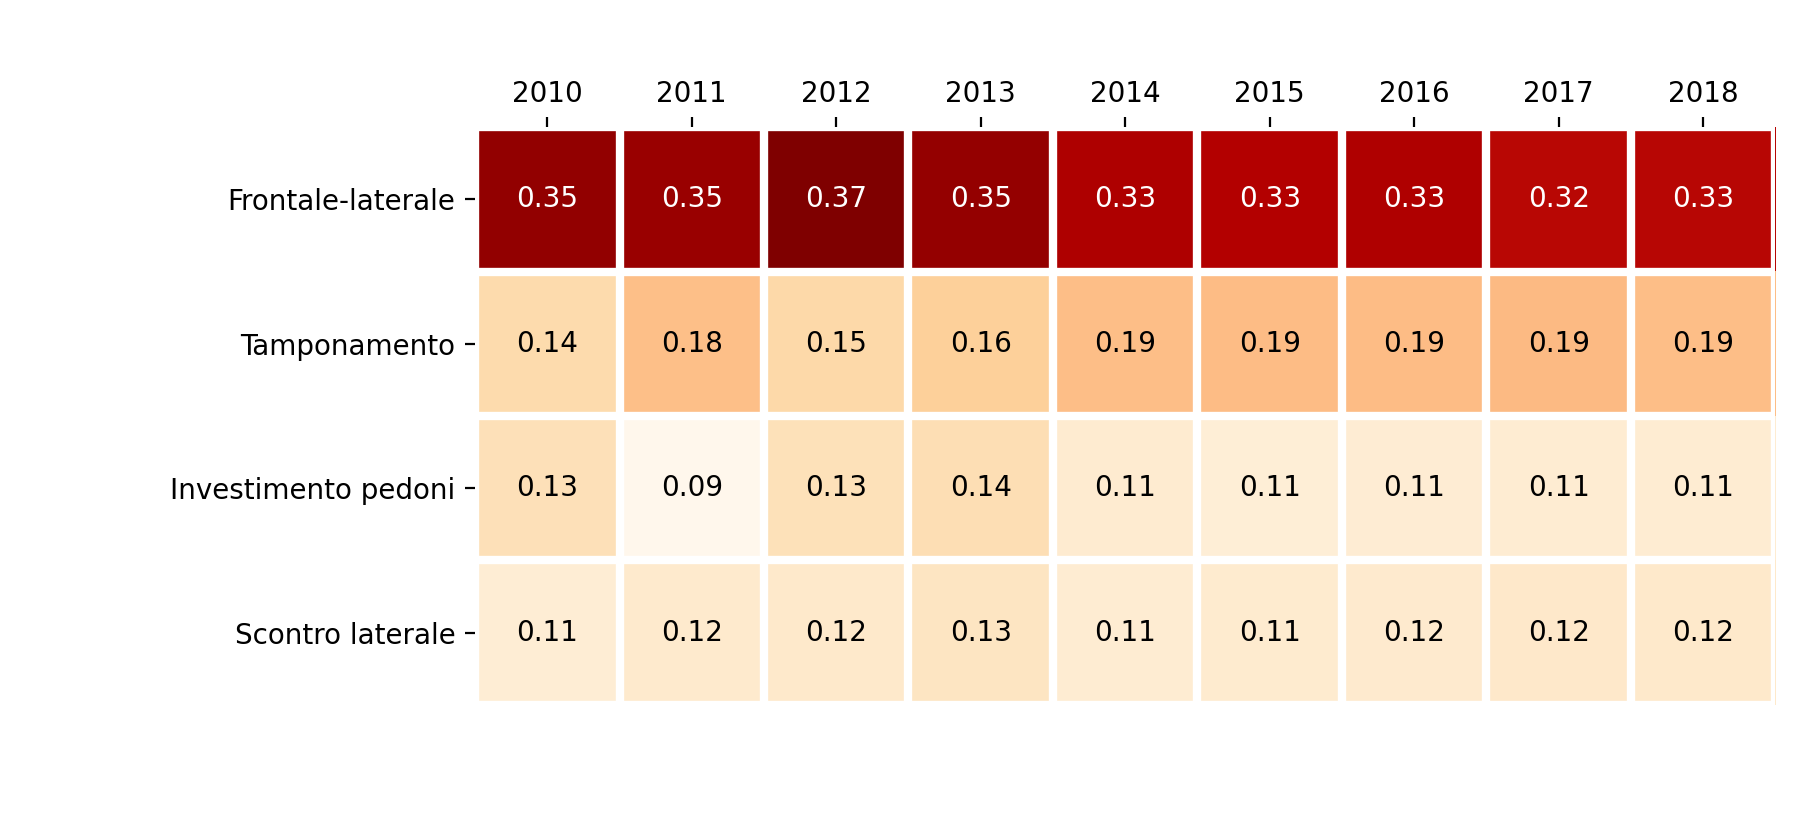
\includegraphics[width=\linewidth]{../src/incidenti/incidenti_senza_coords/localizzazione_incidente/rapporto_tipologie.png}
    \caption{Categorie più frequenti di incidente, divise per anno}
    \label{fig:rapporto-tipologie}
\end{figure}

Per tutte le annate disponibili, le prime due categorie di incidenti rimangono sempre 
le stesse, cioè \columnstyle{Scontro frontale-laterale} e \columnstyle{tamponamento}. 
Anche le frequenze corrispondenti restano molto simili, con la prima 
categoria che rimane attorno al $35$ \% e la seconda attorno al $18$ \%. 

Nel terzo gruppo, d'altra parte, si iniziano ad osservare delle differenze. 

Le tipologie di \columnstyle{investimento} \columnstyle{di} \columnstyle{pedoni} e 
\columnstyle{scontro} \columnstyle{laterale}, 
infatti, si alternano con percentuali simili, attorno al $12$ \%. 

Ciò che è possibile dedurre dalla figura \ref{fig:rapporto-tipologie}, è che non 
sembrano esistere fattori che influenzano il tipo di sinistro più frequente 
nell'arco di un anno.

Se si avessero a disposizione delle informazioni riguardanti il numero e il tipo 
di incroci in una località, sarebbe possibile giustificare 
la maggiore frequenza di sinistri di un tipo rispetto a un altro. 

\subsection{Le tipologie di strada con maggiore indice di mortalità}
\todo{ATOK}

Per tutte queste analisi, in cui si utilizzano le informazioni su tipologie 
di incrocio e di strada, 
sarebbe molto utile avere a disposizione una stima del numero di intersezioni 
per categoria presenti in una certa località, 
per controllare se alcune di queste siano più frequenti di altre. 

Non avendo accesso a questo tipo di dati, si è utilizzato l'indice di 
mortalità per tipologia di sinistro, prendendo spunto dalla sintesi dello 
studio su incidenti stradali, eseguito dall'ente ACI \cite{ACI:2}. 

Nel grafo a barre sul lato sinistro della figura \ref{fig:tipo-intersezioni}, 
sono rappresentati i sinistri in Italia nel 2018, divisi per tipologia 
di strada su cui sono avvenuti. 

\begin{figure}
    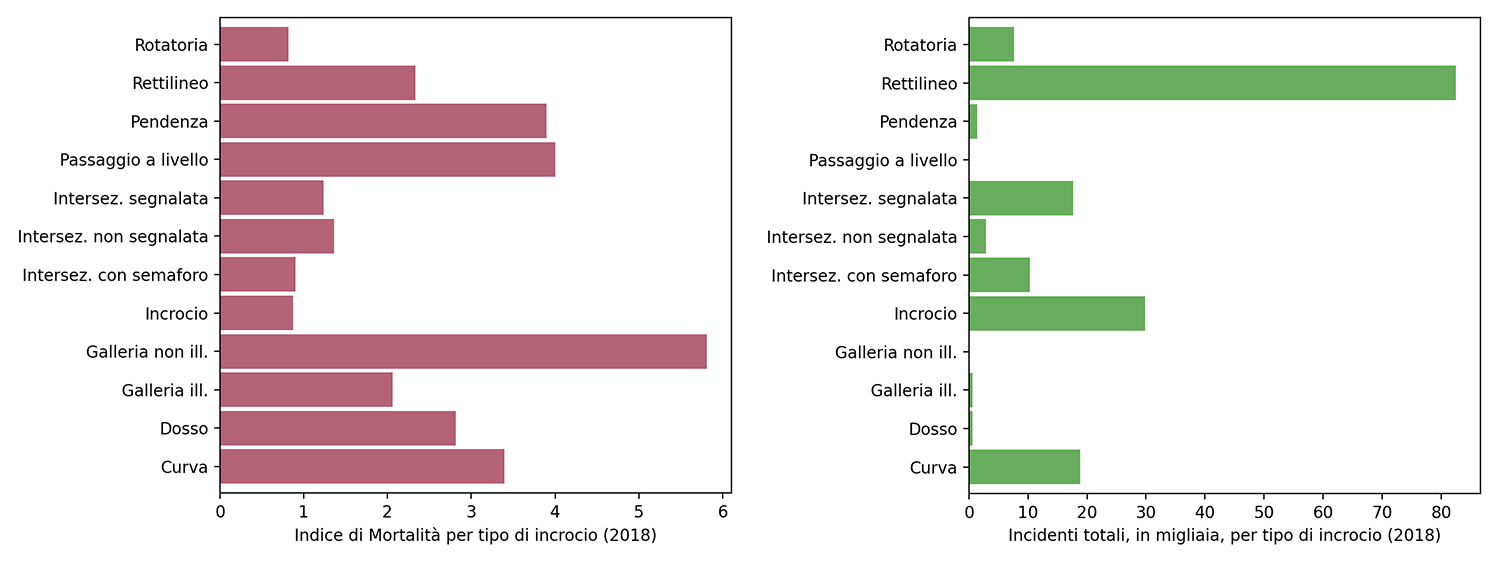
\includegraphics[width=\linewidth]{img_unite/intersezioni_indice_mortalita.png}
    \caption{Percentuale di incidenti e rispettivo indice di mortalità per tipo di strada}
    \label{fig:tipo-intersezioni}
\end{figure}

I risultati sono piuttosto eterogenei, con la maggior parte dei sinistri 
localizzati lungo rettilinei, incroci e curve. 
\`E possibile ipotizzare che, viste le alte velocità raggiunte dai veicoli 
lungo i tratti di strada senza rallentamenti, i risultati calcolati siano corretti, 
e questa categoria sia particolarmente pericolosa. 
D'altro canto, è più probabile che il numero di incidenti di questa tipologia sia dovuto 
all'alta frequenza di strade rettilinee. 

Ulteriore conferma di questa teoria, è data dall'indice di mortalità per tipologia di incrocio, 
riportato nel grafico destro dell'immagine \ref{fig:tipo-intersezioni}, e calcolato tramite la 
formula sottostante. 

\begin{center}
    $Indice\_Mortalita\_Strada\_X = \displaystyle \frac{Numero\_Morti\_Strada\_X}{Numero\_Incidenti\_Strada\_X} * 100$ 
\end{center}

Questo indicatore mostra come, nonostante i rettilinei siano le zone in cui 
avvengono più frequentemente incidenti, questi non siano i tratti di 
strada più pericolosi. 

Nella tabella sottostante sono riportati i valori, sia dell'indice di mortalità, 
sia dell'indice di feriti per tipologia di strada in cui è avvenuto l'incidente. 

\begin{center}
    \def\arraystretch{1.5}%  
    \begin{tabular}{ |c|c|c| } 
    \hline
    Tipo di Incrocio & Indice Mortalità & Indice Feriti \\ 
    \hline
    \rowcolor{TableGray}
    Incrocio                & 0.88 & 143.10 \\
    Rotatoria               & 0.82 & 127.22 \\
    \rowcolor{TableGray}
    Int. segnalata          & 1.24 & 142.14 \\
    Int. con semaforo       & 0.9 & 147.05 \\
    \rowcolor{TableGray}
    Int. non segnalata      & 1.36 & 139.97\\
    Passaggio a livello     & 4.0 & 134.67\\
    \rowcolor{TableGray}
    Rettilineo              & 2.33 & 138.94\\
    Curva                   & 3.39 & 145.26\\
    \rowcolor{TableGray}
    Dosso                   & 2.82 & 156.49\\
    Pendenza                & 3.9 & 134.10\\
    \rowcolor{TableGray}
    Galleria ill.           & 2.06 & 165.87\\
    Galleria non ill.       & 5.81 & 132.59\\
    \hline
    \end{tabular}
\end{center}

Per controllare la validità degli indici calcolati, si è ricavata la correlazione 
tra indice di mortalità, feriti e tra questi ultimi e il numero di incidenti per 
luogo. 
I valori sono riportati nella tabella sottostante: 

\begin{center}
    \def\arraystretch{1.5}%  
    \begin{tabular}{ |c|c| }
        \hline
        \rowcolor{TableGray}
        Tra morti e feriti      & 0.96 \\ 
        Tra incidenti e feriti  & 0.99 \\
        \rowcolor{TableGray}
        Tra incidenti e morti   & 0.96 \\
        \hline
    \end{tabular}
\end{center}

Ne risulta che tutti gli insiemi siano linearmente correlati tra loro. 
Dalla tabella contenente l'indice di feriti, non è possibile dedurre molto, 
in quanto questo indicatore ha valore molto simile tra tutte le categorie. 

Tuttavia, un dettaglio interessante che salta all'occhio, è che il minimo dei due indici, 
coincide nella stessa categoria di strada, 
la rotatoria, informazione che potrebbe essere molto utile per 
la scelta di quale tipologia di incrocio realizzare. 

Per quanto riguarda invece, l'indice di mortalità, è chiaro che sia più alto 
per categorie di incidenti che avvengono ad alte velocità, come vicino a dossi, 
curve e gallerie, rispetto a tratti di strada, come incroci e semafori, 
quando i veicoli stanno ripartendo dopo una fermata.

%\clearpage
\subsection{Le tipologie di sinistro che provocano il maggior numero di feriti}
\todo{ATOK}

Il dataset Istat contiene informazioni riguardanti il numero di persone coinvolte 
in incidenti, in particolare l'età, il sesso e l'esito dove, 
per quest'ultimo campo, si intende lo stato di salute del passeggero 
dopo l'incidente, che può essere: incolume, ferito, deceduto entro 24 ore o entro un mese. 

Può essere utile, pertanto, verificare quali siano le tipologie di 
sinistri che provocano il maggior numero di feriti.

\begin{figure}
    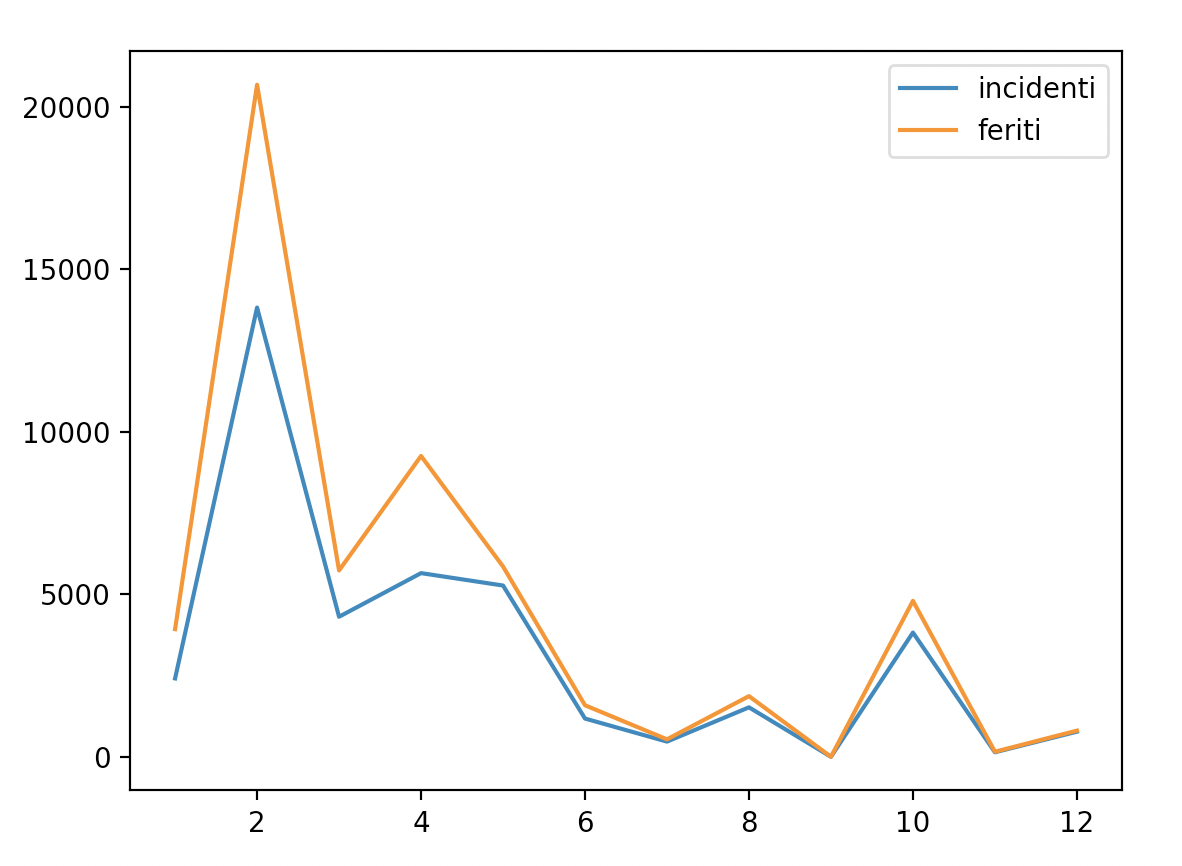
\includegraphics[width=\linewidth]{../src/incidenti/incidenti_senza_coords/natura_incidente/natura_incidente.png}
    \caption{Numero di feriti in base alla natura dell'incidente}
    \label{fig:numero-feriti}
\end{figure}

Dalla figura \ref{fig:numero-feriti} è possibile ipotizzare l'esistenza di categorie 
di sinistri che favoriscono la presenza di un solo ferito, come gli sbandamenti. 
Si arriva a questa conclusione perché la colonna corrispondente, è tra 
le più alte di quelle del primo gruppo (un solo ferito), 
mentre nel secondo gruppo (due feriti), è tra i valori più bassi. 
Al contrario, le colonne corrispondenti al \columnstyle{tamponamento}, sono molto alte 
per ognuno dei quattro gruppi, il che fa pensare che semplicemente avvenga un alto numero 
di sinistri di questo tipo. 

Le percentuali di osservazione degli incidenti nel grafico \ref{fig:numero-feriti} sono 
riportate nella tabella sottostante\footnote{La somma delle percentuali dei tipi di 
sinistri dovrebbe ammontare a 1, ma sono state riportate solo quattro categorie 
interessate, e non tutte.}: 

\begin{center}
    \def\arraystretch{1.5}%  
    \begin{tabular}{ |c|c| } 
    \hline
    Incidente & Percentuale del tipo \\ 
    \hline
    \rowcolor{TableGray}
    Sbandamento       & 0.088 \\
    Tamponamento      & 0.186 \\
    \rowcolor{TableGray}
    Scontro frontale  & 0.056 \\
    Urto con ostacolo & 0.049 \\
    \hline
    \end{tabular}
\end{center}

Avendo a disposizione il numero di sinistri per categoria, è possibile capire 
se il comportamento visibile nel grafico sia dovuto alla maggiore frequenza della tipologie, 
o alla pericolosità del tipo di evento. 

\begin{figure}
    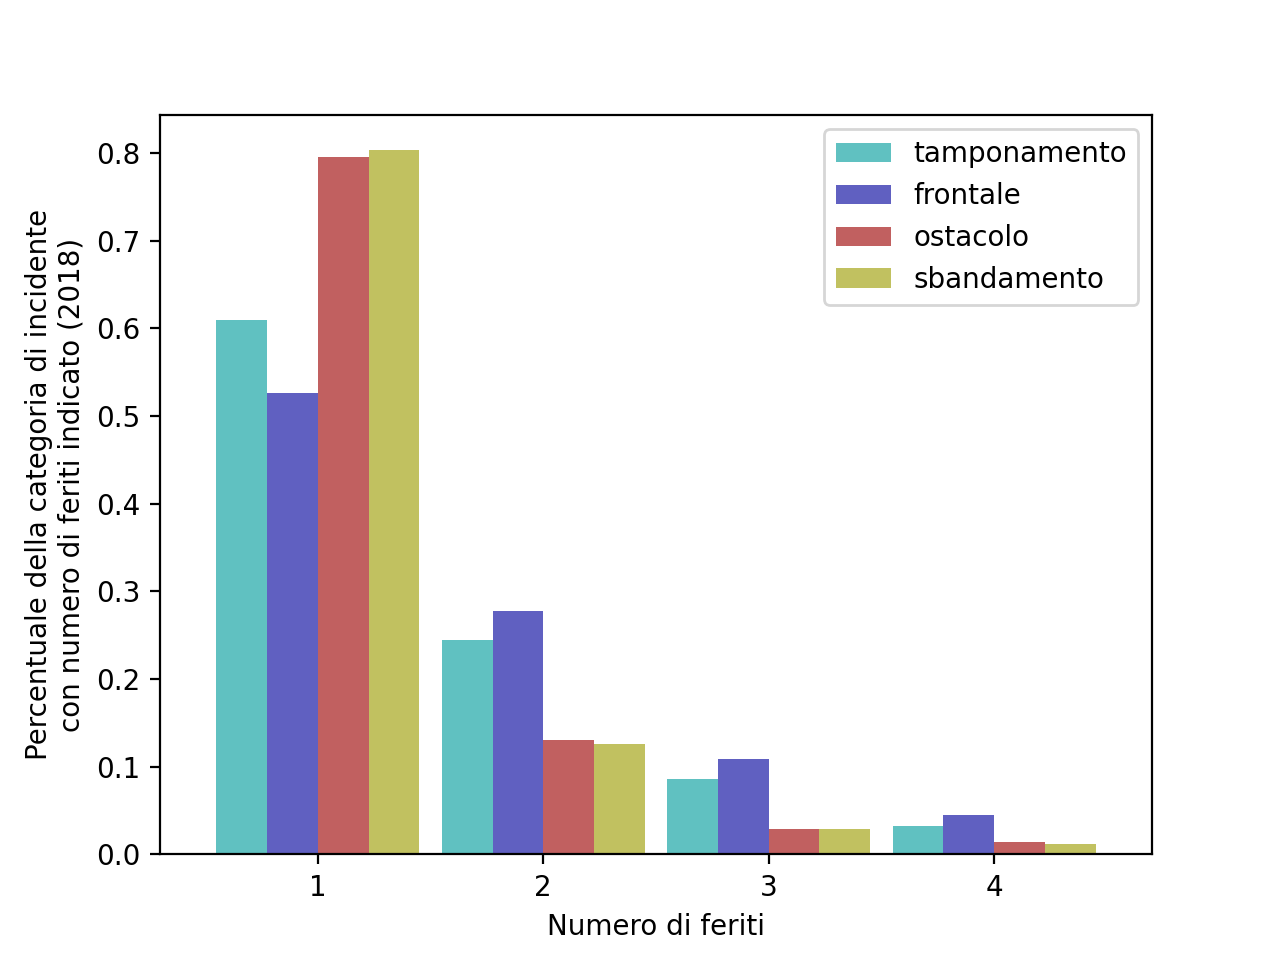
\includegraphics[width=\linewidth]{../src/incidenti/incidenti_senza_coords/natura_incidente/perc_natura_incidente.png}
    \caption{Frequenza del tipo di incidente con numero di feriti, diviso per la percentuale di incidenti della rispettiva categoria}
    \label{fig:perc-numero-feriti}
\end{figure}

La figura \ref{fig:perc-numero-feriti} mostra la distribuzione di incidenti con un dato numero 
di feriti, divisa per la percentuale di sinistri del tipo interessato. 

Avendo a disposizione un indice, corretto in base al volume della categoria, 
si osserva come alcune di queste, come \columnstyle{urto con ostacolo} 
e \columnstyle{sbandamento}, favoriscano una sola persona lesa, mentre altre, 
come i \columnstyle{tamponamenti} e gli \columnstyle{scontri frontali}, presentino 
una maggiore percentuale di eventi con più di un ferito. 

%\clearpage
\subsection{Le tipologie di incroci che favoriscono incidenti con coinvolgimento di pedoni}
\todo{ATOK}

Il dataset Istat fornisce varie informazioni riguardanti i pedoni coinvolti in un 
incidente, tramite le colonne sottostanti, ripetute quattro volte, 
una per ogni persona interessata.


\lighttext{(\\
\indent\columnstyle{pedone\_morto\_X\_\_sesso}, \\
\indent\columnstyle{pedone\_morto\_X\_\_et\_}\footnote{I label contenenti \quotestyle{et} indicano l'età dei pedoni}, \\
\indent\columnstyle{pedone\_ferito\_X\_\_sesso}, \\
\indent\columnstyle{pedone\_ferito\_X\_\_et\_}, \\
)\footnote{Questi campi sono ripetuti quattro volte, rimpiazzando la 'X' 
con l'indice della colonna}} 


Rimanendo sul tema dei capitoli precedenti, 
si potrebbe verificare quali tipologie di incrocio coinvolgono 
il maggior numero di pedoni.

\begin{figure}
    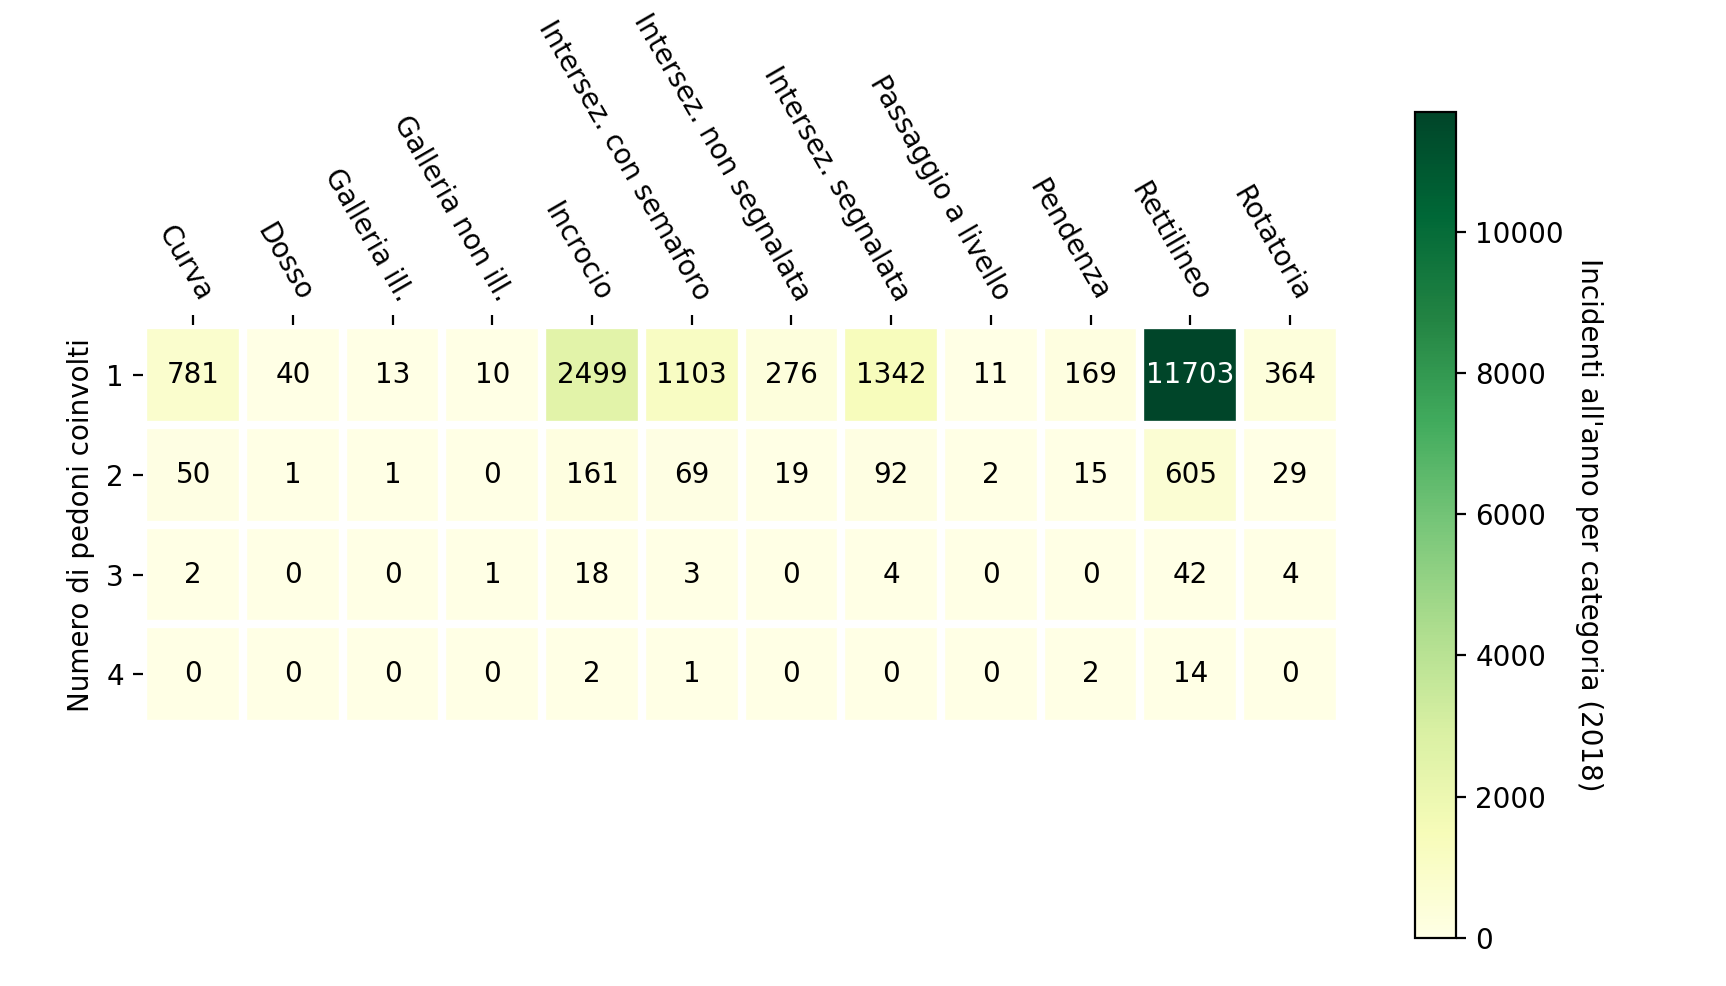
\includegraphics[width=\linewidth]{../src/incidenti/incidenti_senza_coords/pedoni/pedoni_incroci.png}
    \caption{Tipologia di intersezioni e pedoni coinvolti}
    \label{fig:pedoni-intersezioni}
\end{figure}

La figura \ref{fig:pedoni-intersezioni} mostra il numero di incidenti, 
ordinati in base alla tipologia di intersezione in cui sono avvenuti 
e al numero di persone coinvolte. 

Come si era già osservato nell'istogramma \ref{fig:tipo-intersezioni}, nella nuova 
figura emerge l'alto numero di rettilinei. 
Analogamente all'analisi precedente, si è inclini a pensare che il valore 
elevato di questa categoria sia dovuto all'alto 
numero di tratti di strada dritti, tuttavia confrontando le due immagini, 
la frequenza di sinistri su rettilineo è quasi cinque 
volte il valore della seconda posizione. 

Questa alta quantità di incidenti fa pensare che esista un qualche fattore 
che comporti maggiore coinvolgimento di pedoni lungo rettilinei, come 
l'alta velocità dei veicoli. 

\begin{figure}
    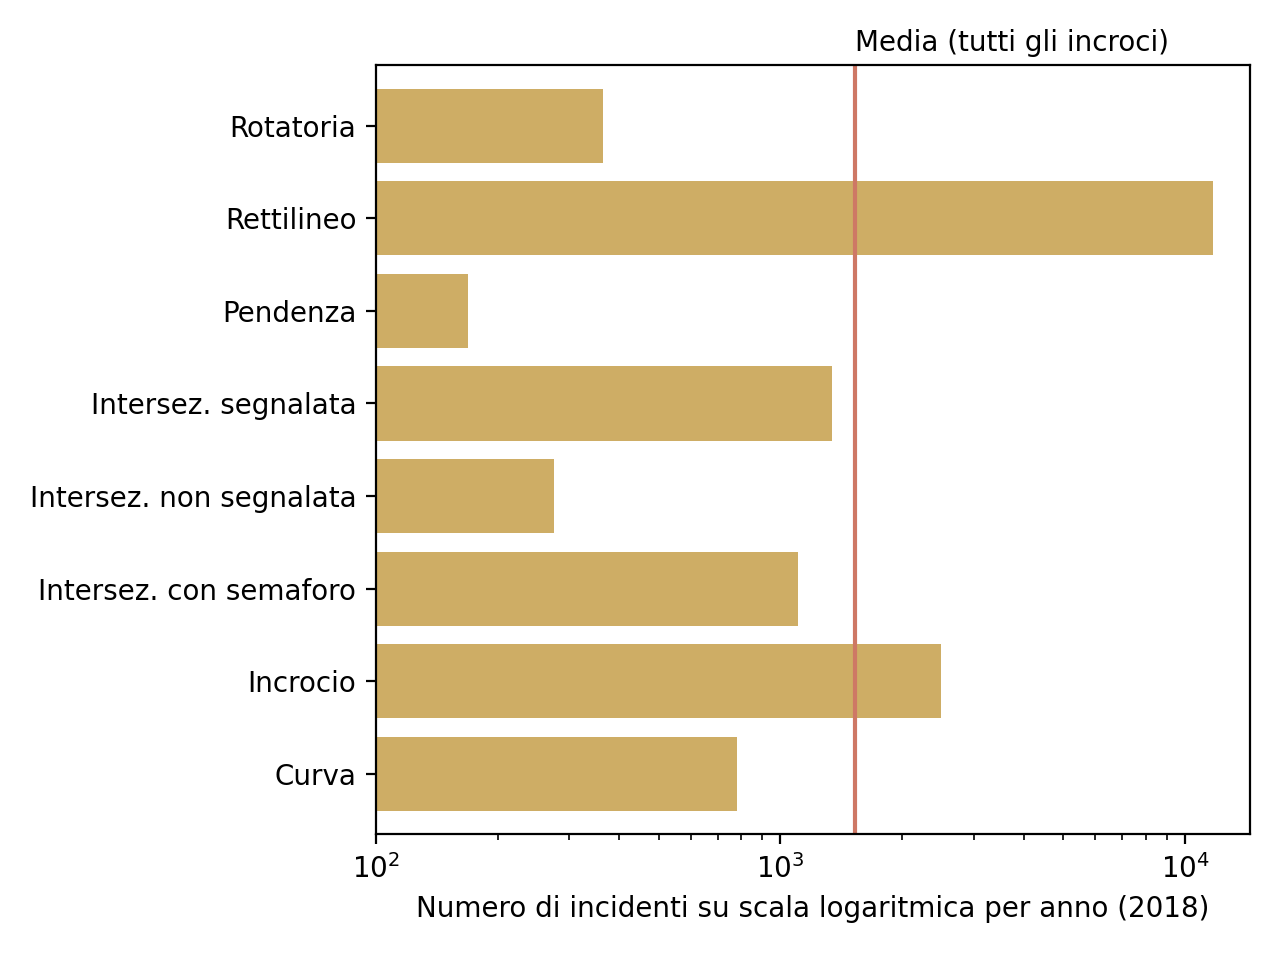
\includegraphics[width=\linewidth]{../src/incidenti/incidenti_senza_coords/pedoni/pedoni_log.png}
    \caption{Tipologia di intersezioni e pedoni coinvolti, ignorando le categorie con valori più bassi}
    \label{fig:pedoni-no-rett}
\end{figure}

In figura \ref{fig:pedoni-no-rett} sono state 
escluse le categorie con i valori 
più bassi\footnote{Sono state rimosse tutte le categorie con valore minore di 
150 incidenti all'anno}, 
in particolare \columnstyle{Dosso}, \columnstyle{Galleria ill.}, 
\columnstyle{Galleria non ill.,} e \columnstyle{Passaggio a livello}. 

Il grafico ottenuto è più bilanciato, con \columnstyle{incroci} e 
\columnstyle{intersezioni non segnalate} che spiccano come tipologie di strada con 
maggiore coinvolgimento di pedoni e le restanti categorie non troppo distanti, 
sempre in coda a \columnstyle{rettilineo}. 

Va specificato che l'istogramma \ref{fig:pedoni-no-rett} è stato realizzato utilizzando, 
nell'asse delle ascisse, una scala logaritmica, poiché il numero di pedoni coinvolti 
su rettilineo è un ordine di grandezza maggiore rispetto alla media, e 
comporta che i valori di tutti gli altri gruppi siano \quotestyle{appiattiti} 
verso l'asse delle ordinate. 

A differenza dell'analisi precedente sui tratti di strada più pericolosi, 
escludendo di proposito i rettilinei, emerge un'immagine decisamente diversa. 
Non sembra, infatti, più essere l'alta velocità la causa di incidenti convolgenti pedoni, 
quanto invece la scarsa visibilità reciproca, dovuta per esempio a curve, siepi o a 
segnaletica non ben evidenziata.

%\clearpage
\subsection{Differenze nell'età dei pedoni coinvolti in incidenti}
\todo{ATOK}

Può sembrare scontato che, qualora coinvolti in un incidente, un pedone ventenne e 
uno settantenne non abbiano la stessa probabilità di rimanere feriti. 
I dati a disposizione possono aiutare ad evidenziare le differenze.

I campi utilizzati, provenienti dal dataset Istat, sono quelli contrassegnati 
con il label 
\columnstyle{pedone\_X\_ferito\_età}\footnote{Nel dataset sono presenti quattro colonne per 
annotare l'età dei pedoni coinvolti, dove l'indice della colonna sostituisce la 'X' nel label.}. 

\begin{figure}
    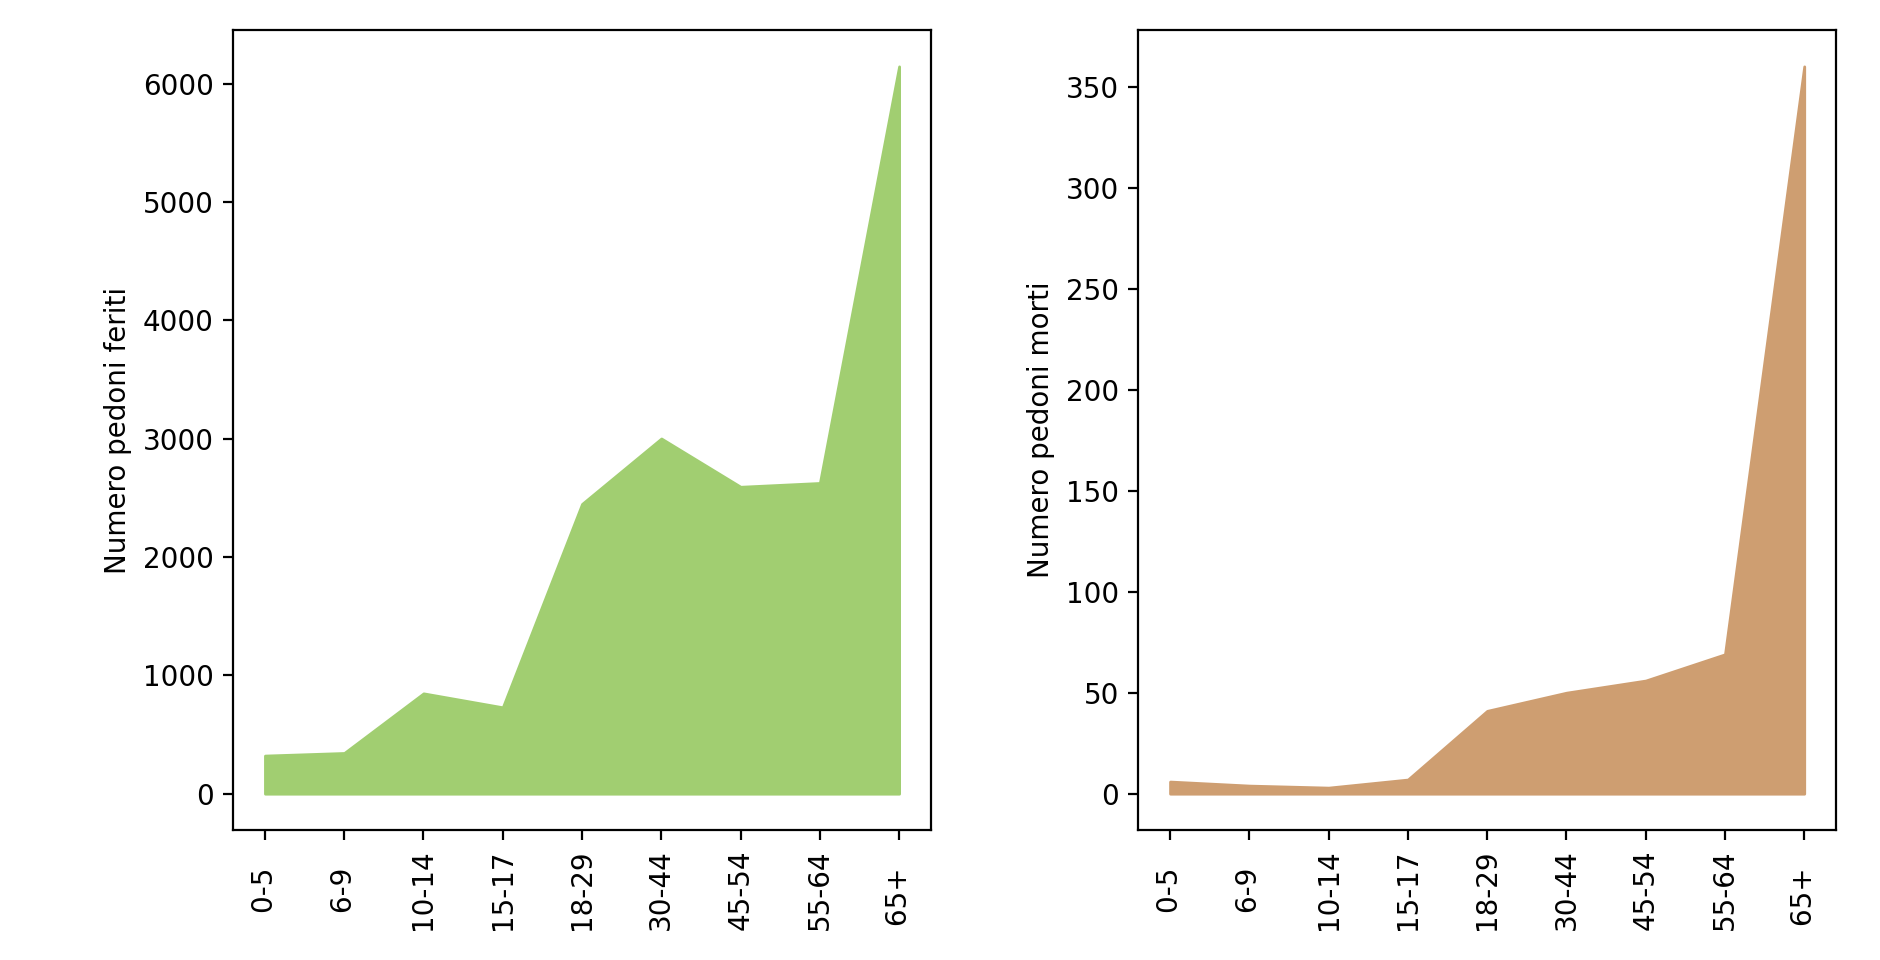
\includegraphics[width=\linewidth]{../src/incidenti/incidenti_senza_coords/pedoni/eta_pedoni_iniziale.png}
    \caption{Frequenze di coinvolgimento di pedoni in incidenti per fascia di età}
    \label{fig:eta-pedoni-iniziale}
\end{figure}

Dal grafico \ref{fig:eta-pedoni-iniziale} si osserva come la fascia più colpita 
sia quella dei \columnstyle{65+} anni, tuttavia esiste un secondo picco, nell'istogramma 
dei pedoni feriti, che comprende le persone tra i trenta e cinquantaquattro anni di età. 

L'ampiezza delle fasce, purtroppo, non è omogenea, determinando una difficoltà 
nella valutazione dei dati.
La categoria 
\columnstyle{30-44}, per esempio abbraccia quindici anni, mentre 
\columnstyle{18-20} ne contiene solo due. 

\begin{code}[language=Python]
numero_anni = np.array([5, 5, 5, 3, 10, 15, 10, 10, 20])

pedoni_feriti_vals = pedoni_feriti.values / numero_anni
pedoni_morti_vals = pedoni_morti.values / numero_anni
\end{code}

\begin{figure}
    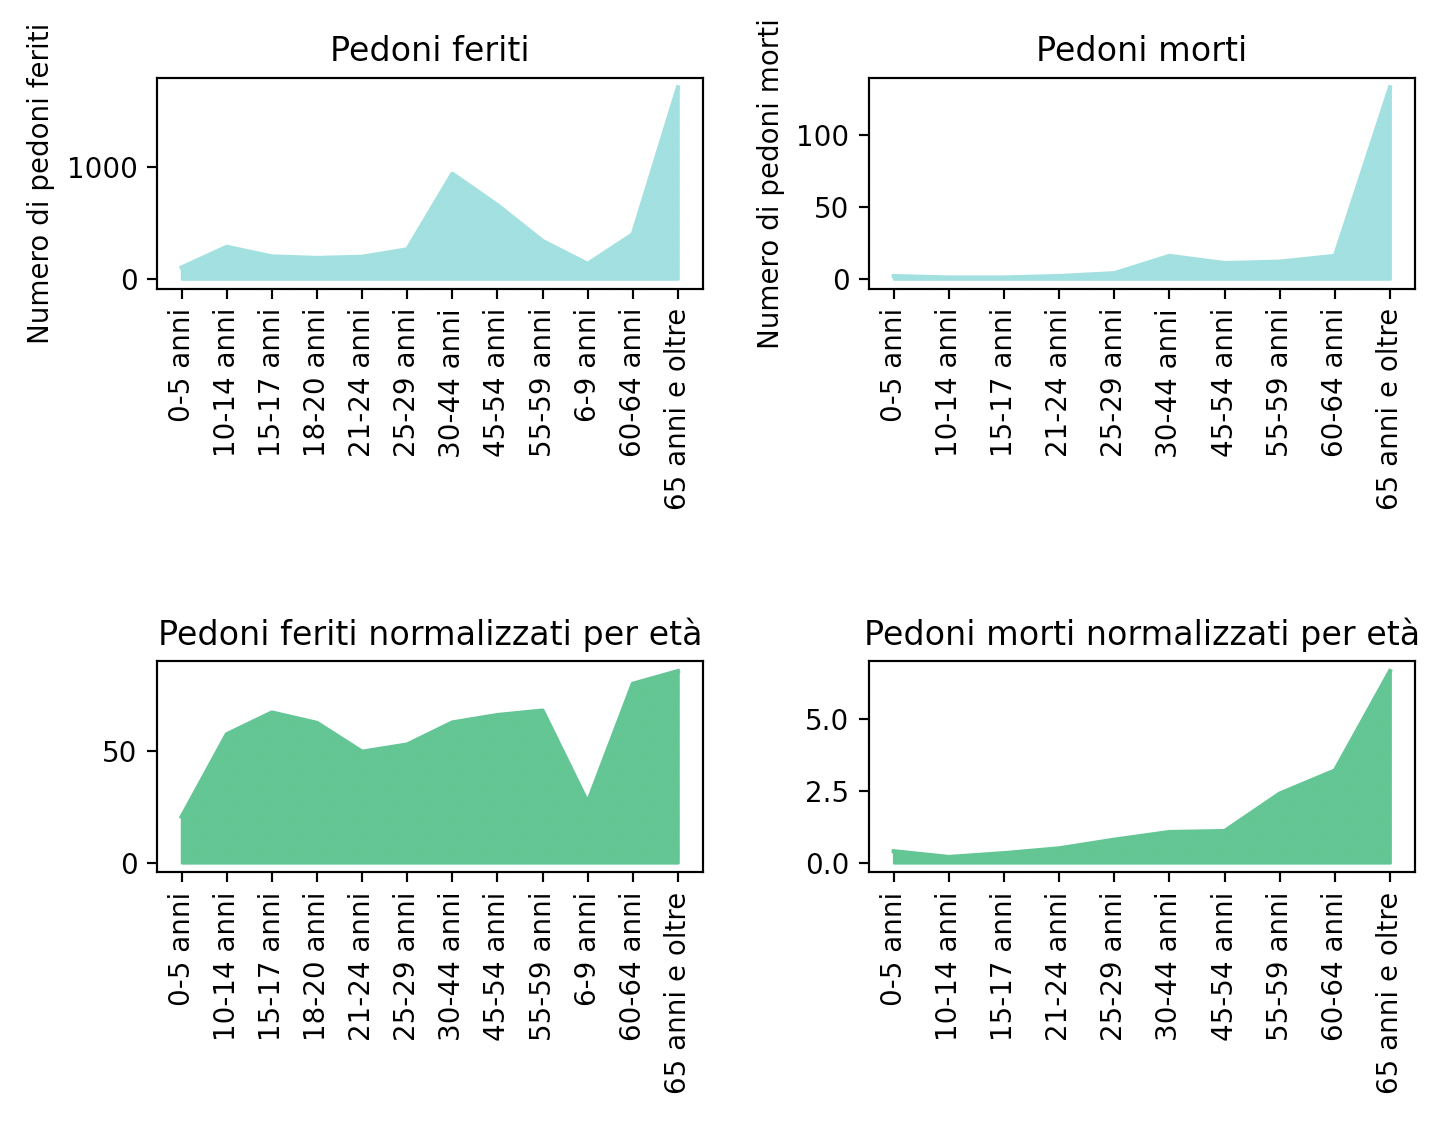
\includegraphics[width=\linewidth]{../src/incidenti/incidenti_senza_coords/pedoni/eta_pedoni.png}
    \caption{Fasce di età dei pedoni coinvolti in incidenti, normalizzate per numero di anni 
    presenti nella categoria}
    \label{fig:eta-pedoni}
\end{figure}

Se si normalizza per anni contenuti in ogni categoria, ipotizzando un numero 
costante di persone di ogni età\footnote{La normalizzazione tiene conto 
che la fascia di età \columnstyle{65+} valga venti anni.}, 
si ottiene il grafico visibile in figura \ref{fig:eta-pedoni}. 
Per quanto riguarda i pedoni feriti, 
questa rappresentazione è molto differente, infatti, 
ignorando gli individui più giovani, tutte le altre fasce sono coinvolte 
in modo omogeneo, con un picco nella categoria \columnstyle{65+ anni}. 
D'altra parte, la figura destra, contenente i morti per fascia di età, 
non subisce un grande cambiamento, mantenendo il punto di massimo nei 
pedoni più anziani. 

D'altra parte in Italia il numero di individui con 
la stessa età non è costante, anzi, le percentuali di popolazione per fascia, 
trovate sul sito Tuttitalia \cite{TUTTITALIA:1}, non sono particolarmente omogenee, 
come si evince dalla tabella sotto riportata: 

\begin{center}
    \def\arraystretch{1.5}%  
    \begin{tabular}{ |c|c| } 
    \hline
    Età & Percentuale Popolazione \\ 
    \hline
    \rowcolor{TableGray}
    0-5     & 3.9 \% \\ 
    6-9     & 4.5 \% \\
    \rowcolor{TableGray}
    10-14   & 4.8 \% \\
    15-17   & 3.1 \% \\
    \rowcolor{TableGray}
    18-20   & 2.8 \% \\ 
    21-24   & 4   \% \\
    \rowcolor{TableGray}
    25-29   & 5.3 \% \\
    30-44   & 19  \% \\
    \rowcolor{TableGray}
    45-54   & 18.2 \% \\ 
    55-59   & 7.3 \% \\
    \rowcolor{TableGray}
    60-64   & 6.4 \% \\
    65$+$   & 19.3 \% \\
    \hline
    \end{tabular}
\end{center}

Visto che gli insiemi di persone del sito e quelle del dataset Istat non coincidono, 
si è dovuto, in alcuni casi sommare, in altri suddividere, 
i dati provenienti da Tuttitalia. 
Nel caso occorra spezzare una fascia, è necessario stimare la percentuale 
di popolazione con determinata età. 
Un esempio è la categoria dei \columnstyle{15-19} anni; 
i dati Istat hanno un insieme per \columnstyle{15-17} anni e un altro per 
\columnstyle{18-29} anni, 
bisogna dunque spostare i diciotto e i diciannovenni dal primo al 
secondo gruppo. 
In questi casi, si è semplicemente assunto che la quantità di individui sia omogeneamente 
divisa per età, cioè in \columnstyle{15-19 anni} si abbia lo stesso numero di 
quindicenni e sedicenni. 
Seguendo questo principio, per collocare le due annate nella categoria successiva, 
è opportuno dividere la cardinalità\footnote{Il numero di elementi presenti nell'insieme.} 
dell'insieme \columnstyle{15-19} per cinque e moltiplicare per due. 
Il risultato ottenuto va aggiunto alla fascia \columnstyle{18-29}. 

\begin{code}
correct_order = ['0-5  ', '6-9  ', '10-14', '15-17', '18-29', '30-44', '45-54', '55-64','65+  ']
perc_fascia = np.array( [3.9, 4.5, 4.8, 3.1, 12.1, 19, 18.2, 13.7, 19.3]) / 100

pedoni_feriti_vals = pedoni_feriti.values / perc_fascia
pedoni_morti_vals = pedoni_morti.values / perc_fascia
\end{code}

\begin{figure}
    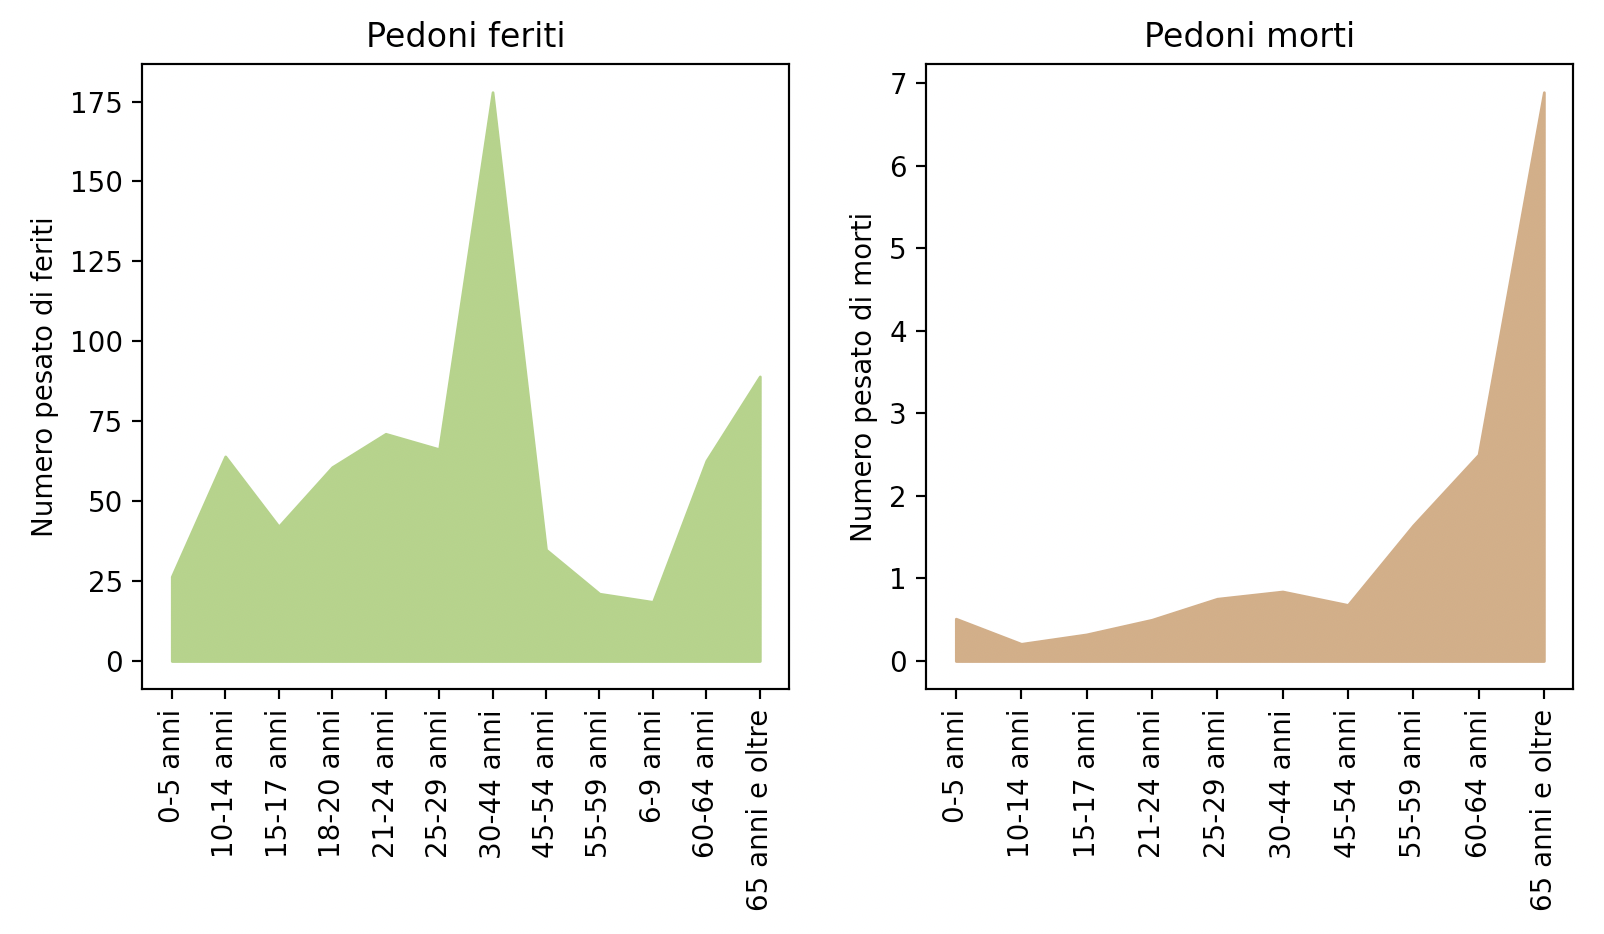
\includegraphics[width=\linewidth]{../src/incidenti/incidenti_senza_coords/pedoni/eta_pedoni_norm.png}
    \caption{Fasce di età dei pedoni coinvolti in incidenti, normalizzate tramite percentuale di popolazione}
    \label{fig:eta-pedoni-norm}
\end{figure}

Una volta corretta l'immagine precedente, si ottiene la figura \ref{fig:eta-pedoni-norm} 
dove, soprattutto nella rappresentazione di destra, è presente una curva particolarmente alta 
nelle fasce più anziane, e un secondo picco nella categoria \columnstyle{18-29 anni}. 

Anche nel grafico di sinistra è visibile la stessa impennata in corrispondenza 
del gruppo \columnstyle{18-29}, mentre in quello dei \columnstyle{65+} la 
percentuale non risulta particolarmente alta. 

Si può ipotizzare che l'incremento di deceduti nelle fasce più anziane, sia dovuto al 
fatto che questi ultimi siano più propensi all'essere feriti in un incidente. 
Nonostante ciò, le categorie centrali, in particolare \columnstyle{18-29 anni}, 
una volta aggiustati i calcoli per popolazione standard, sembrano essere comunque 
quelle più coinvolte in sinistri. 

\subsection{Differenze nell'età dei conducenti che causano sinistri}
\todo{ATOK}

Come specificato nel capitolo precedente, il dataset Istat dispone di 
informazioni sull'età dei pedoni coinvolti. Analogamente a questi, 
sono anche presenti gli stessi dati, ma riguardanti i passeggeri e il conducente dei 
veicoli. 

\`E dunque possibile verificare se esistono fasce di età di persone alla guida, 
che provocano un numero di sinistri particolarmente alto. 

\begin{figure}
    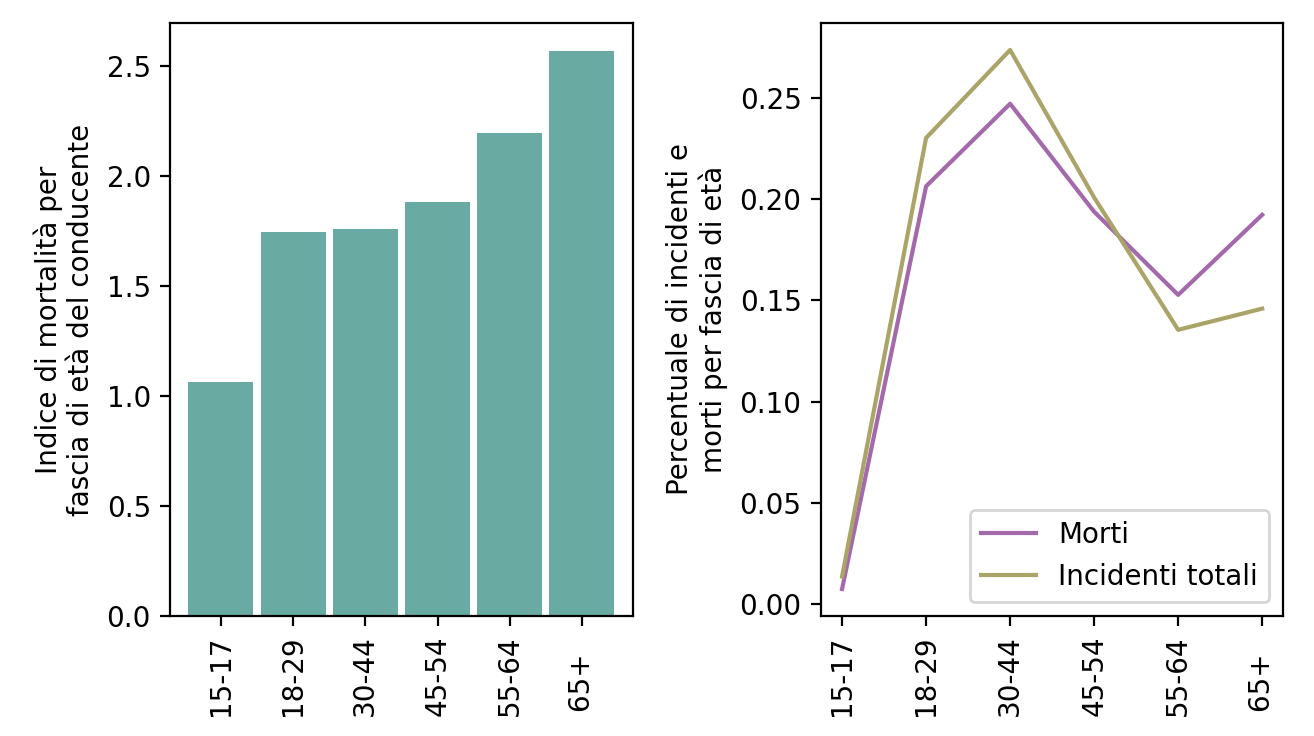
\includegraphics[width=\linewidth]{../src/incidenti/incidenti_senza_coords/mortalita/indice_mortalita_eta.png}
    \caption{Indice di mortalità degli incidenti, divisi in base all'età del conducente}
    \label{fig:indice-mortalita-eta}
\end{figure}

In primo luogo, il grafico destro nella figura \ref{fig:indice-mortalita-eta} contiene 
la percentuale di incidenti totali commessi per fascia di età del conducente, insieme 
al numero di morti in questi eventi\footnote{Ogni punto contiene sinistri in 
cui il conducente rientra nella fascia di età, la persona deceduta tuttavia potrebbe non 
essere la persona alla guida}. 

In particolare, più di un quarto dei sinistri totali coinvolgono persone nella 
fascia d'età \columnstyle{30-44 anni} mentre, il gruppo \columnstyle{15-17} sembrerebbe 
essere molto più responsabile alla guida. Il numero di conducenti che rientrano 
in queste categorie, tuttavia, deve essere particolarmente basso, in quanto si 
parla di ragazzi con patenti di tipo A1\footnote{Patenti conseguibili a partire dai 16 anni, 
che permettono la guida di motocicli con potenza ridotta}. 

Nell'istogramma in figura \ref{fig:indice-mortalita-eta}, invece, 
è rappresentato l'indice di mortalità di questi incidenti, 
calcolato utilizzando la formula: 

\begin{center}
    $Indice\_Mortalita\_X = \displaystyle \frac{Numero\_Morti\_X}{Numero\_Incidenti\_X} * 100$ 
\end{center}

Il risultato calcolato, presente nel grafico, aumenta al crescere dell'età, 
e sembra essere confermato dalla stima realizzata nello studio 
ACI del 2018 sugli incidenti stradali \cite{ACI:3}. 

Tuttavia, come già spiegato nei capitoli precedenti, il gruppo \columnstyle{30-44} 
contiene quindici anni, invece che solamente due, come quello dei \columnstyle{15-17}. 

Sarebbe quindi opportuno normalizzare la percentuale di incidenti commessi, 
con una stima del numero di guidatori nella rispettiva fascia di età. 

\begin{code}
perc_fascia = np.array( [3.1, 12.2, 19, 18.2, 13.7, 19.3]) / 100

incidenti_per_eta /= perc_fascia
morti_per_eta /= perc_fascia

indice_mortalita = morti_per_eta * 100 / incidenti_per_eta
\end{code}

\begin{figure}
    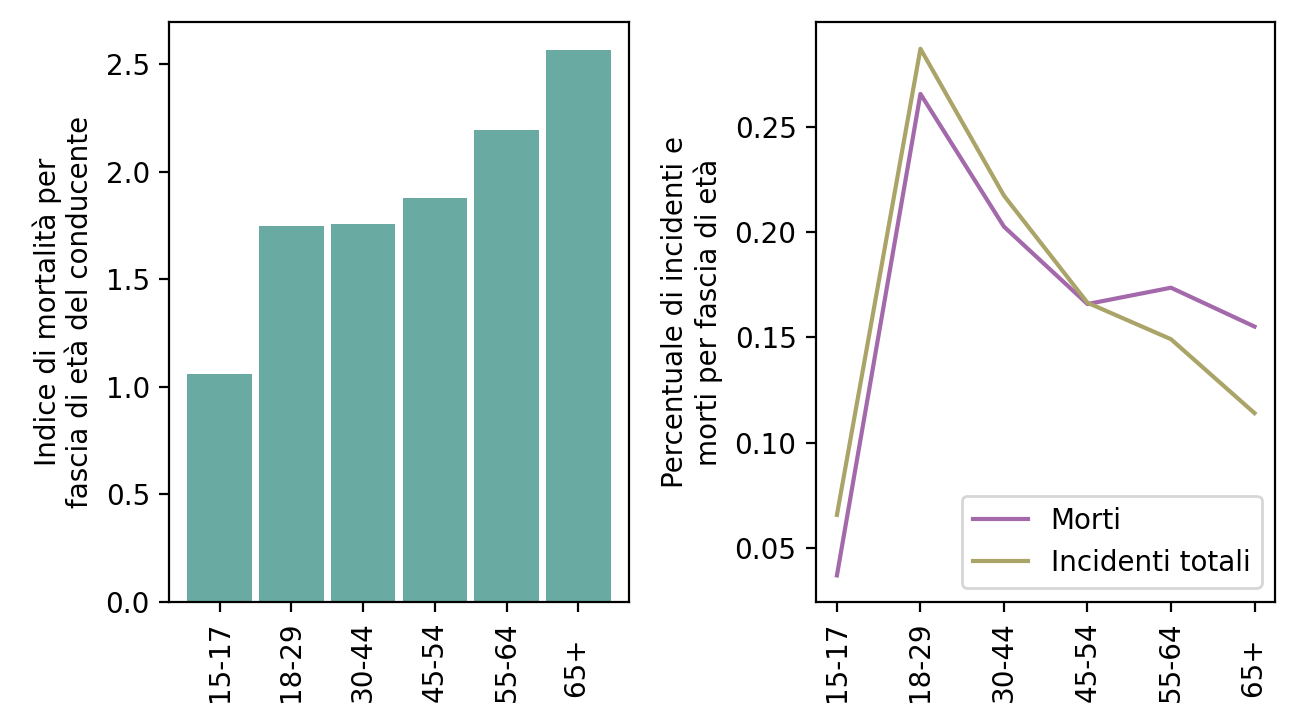
\includegraphics[width=\linewidth]{../src/incidenti/incidenti_senza_coords/mortalita/indice_mort_norm.png}
    \caption{Indice di mortalità degli incidenti, normalizzato per popolazione standard}
    \label{fig:indice-mort-norm}
\end{figure}

Una volta normalizzato per la popolazione standard in Italia, il numero di incidenti per 
fascia di età, nel grafico destro della figura \ref{fig:indice-mort-norm}, mostra che  
si causano più sinistri nella categoria \columnstyle{18-29 anni}, 
con un calo nei gruppi successivi. 

D'altra parte, l'indice di mortalità non subisce alcun cambiamento, 
poiché è realizzato tramite 
un rapporto in cui i fattori sono stati divisi per costanti uguali per ogni fascia. 

%\clearpage
\section{Dati ACI}

I dati trovati sul sito di ACI sono inizialmente separati in due file in 
base al tipo di strada in cui è avvenuto l'incidente, autostrade o strade provinciali. 
I due gruppi, a loro volta sono rispettivamente divisi in categorie, a seconda 
dell'informazione contenuta, come incidenti con 
località\footnote{Per località si intende il nome della via in cui è avvenuto il sinistro}, 
per comune, per mese, per giorno della settimana o per ora. 

\subsection{Regioni italiane con maggior numero di incidenti}
\todo{ATOK}

I dati ACI, in particolare i file riguardanti la 
localizzazione degli incidenti, contengono informazioni che è  
possibile suddividere per regione e per provincia. 

Grazie al dataset geojson di Guglielmo 
Celata\footnote{\url{https://github.com/openpolis/geojson-italy}}, 
sono state realizzate le mappe in figura \ref{fig:incidenti-per-regione}, 
che rappresentano rispettivamente, le regioni con più incidenti 
sulle strade provinciali e sulle autostrade, nell'anno 2018. 

\begin{figure}
    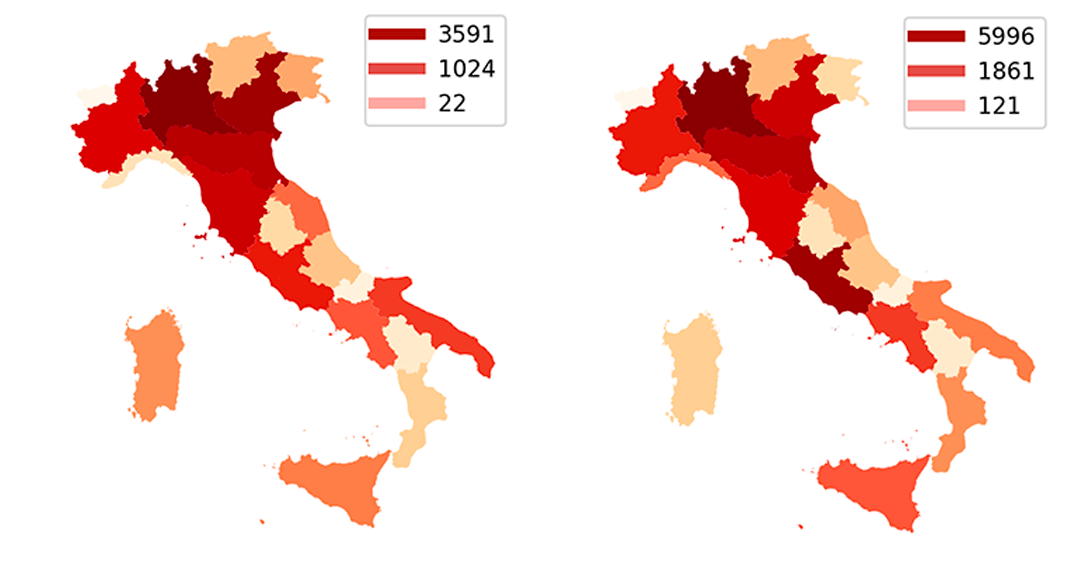
\includegraphics[width=\linewidth]{img_unite/incidenti_autostrade_provinciali.png}
    \caption{Incidenti su autostrade e su strade provinciali nel 2018}
    \label{fig:incidenti-per-regione}
\end{figure}

Ovviamente il Nord Italia detiene il primato, 
soprattutto nelle regioni di Lombardia, Veneto e Emilia Romagna. 
Emerge poi il Lazio, dove la maggior parte dei sinistri avvengono su autostrade, 
in quanto il volume di questi, in figura \ref{fig:incidenti-per-regione}, 
è nella media nella prima mappa, mentre è il valore massimo nella seconda. 

\begin{figure}
    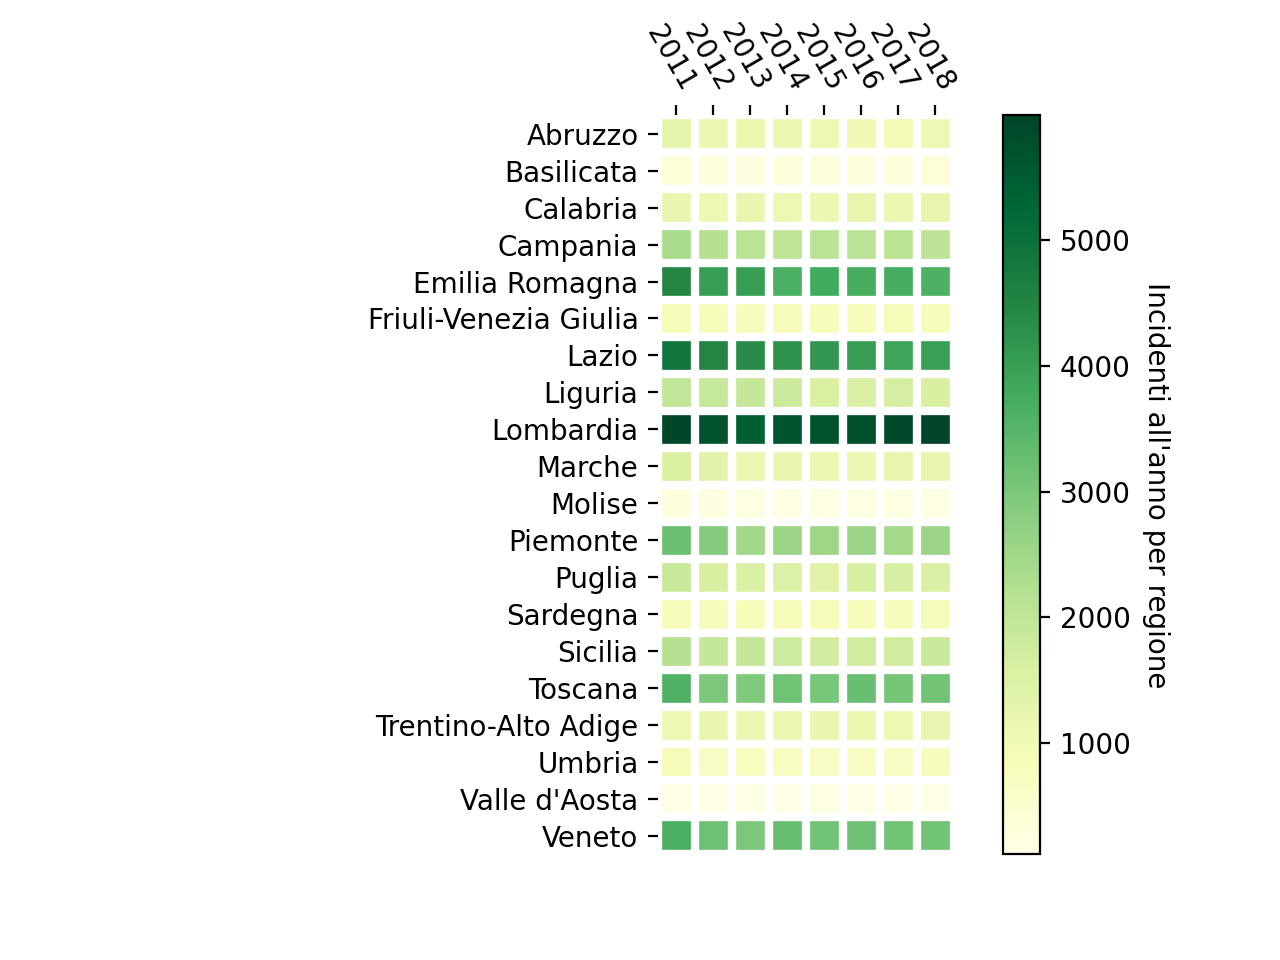
\includegraphics[width=\linewidth]{../src/incidenti/incidenti_aci/mappe_regioni/regioni_heatmap.png}
    \caption{Incidenti all'anno per regione su strade provinciali}
    \label{fig:regione-heatmap}
\end{figure}

Per quanto riguarda, invece, il numero di incidenti 
nella heatmap \ref{fig:regione-heatmap}, 
si nota che questi non cambiano molto di anno in anno, e le regioni con maggiore quantità 
di eventi rimangono sempre Lombardia e Veneto. 

Per controllare le tendenze di incremento e decremento di sinistri per regione, 
si è calcolata la deviazione standard\footnote{Deviazione standard: 
misura della distanza dei dati di un campione dalla media 
(fonte: \citetitle{PROB_E_STATISTICA:1}\cite{PROB_E_STATISTICA:1}, 
capitolo: Statistica descrittiva, pagine: 25-27)}. 
Risulta che la regione con maggiori differenze di incidenti di anno in anno 
è il Lazio, con $324$, mentre quella con minore 
variazione è la Valle d'Aosta, con $8$. 

I grafici precedenti, soprattutto le heatmap regionali, non tengono conto del 
volume del automobili in viaggio. 
Non avendo informazioni riguardanti il traffico in tutta Italia, 
e non potendo usare gli accessi all'area C, validi solo a Milano, si sono realizzate 
delle stime tramite il numero di patentati per regione. 

Va sottolineato che una stima eseguita con tale modalità, 
non potrà essere particolarmente 
sicura, vista la mobilità tra luoghi di residenza, di 
lavoro o di studio che può decisamente falsare la localizzazione dei sinistri.

\begin{figure}
    \hfill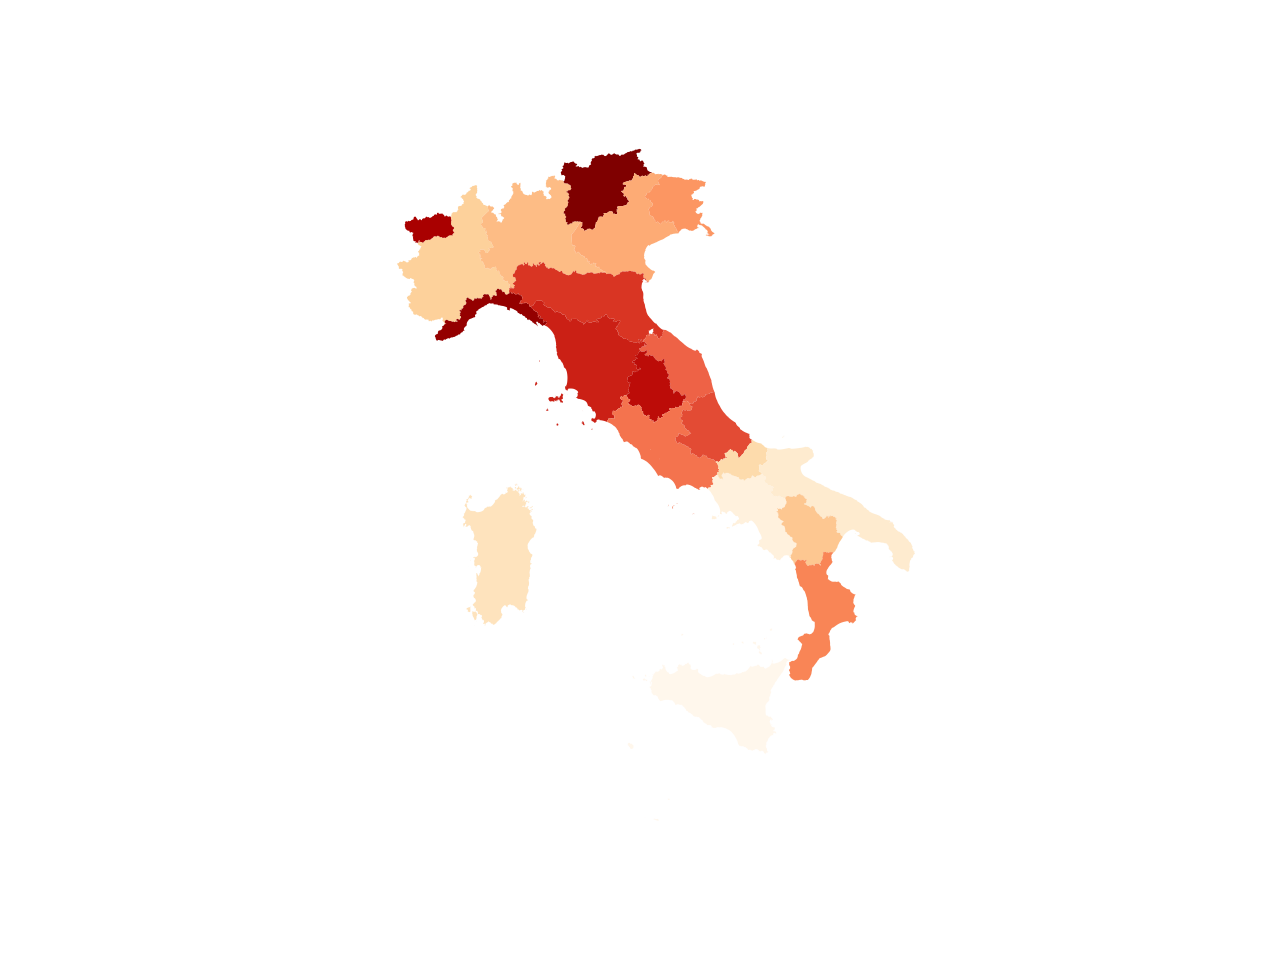
\includegraphics[width=\linewidth]{../src/incidenti/incidenti_aci/mappe_regioni/incidenti_patenti_italia.png}\hspace*{\fill}
    \caption{Incidenti e patentati per regione}
    \label{fig:incidenti-patentati}
\end{figure}

Nel rapporto tra sinistri e patentati per regione, 
visibile in figura \ref{fig:incidenti-patentati}, 
si osserva una chiara distinzione tra Nord, Centro e Sud Italia. 
A cosa è dovuta questa ampia disparità?

Nella seguente tabella sono riportate le medie di incidenti annuali, 
e quella dei patentati per regione. 

\begin{center}
    \def\arraystretch{1.5}%  
    \begin{tabular}{ |c|c|c| } 
    \hline
    Zona & Media Incidenti & Patentati (in Milioni) \\ 
    \hline
    \rowcolor{TableGray}
    Nord    &   2470 &   2.28 \\ 
    Centro  &   2395 &   1.97 \\ 
    \rowcolor{TableGray}
    Sud     &   1145 &   1.57 \\ 
    \hline
    \end{tabular}
\end{center}

L'istogramma \ref{fig:incidenti-patentati-bar} è stato suddiviso tra nord, 
centro e sud Italia per facilitare la lettura, e indica le percentuali di sinistri e 
patentati per la rispettiva regione. 
\`E subito osservabile che, nella maggior parte delle zone del centro, 
la frequenza di incidenti supera quella delle patenti, 
mentre al sud avviene il fenomeno opposto. 

\begin{figure}
    \hfill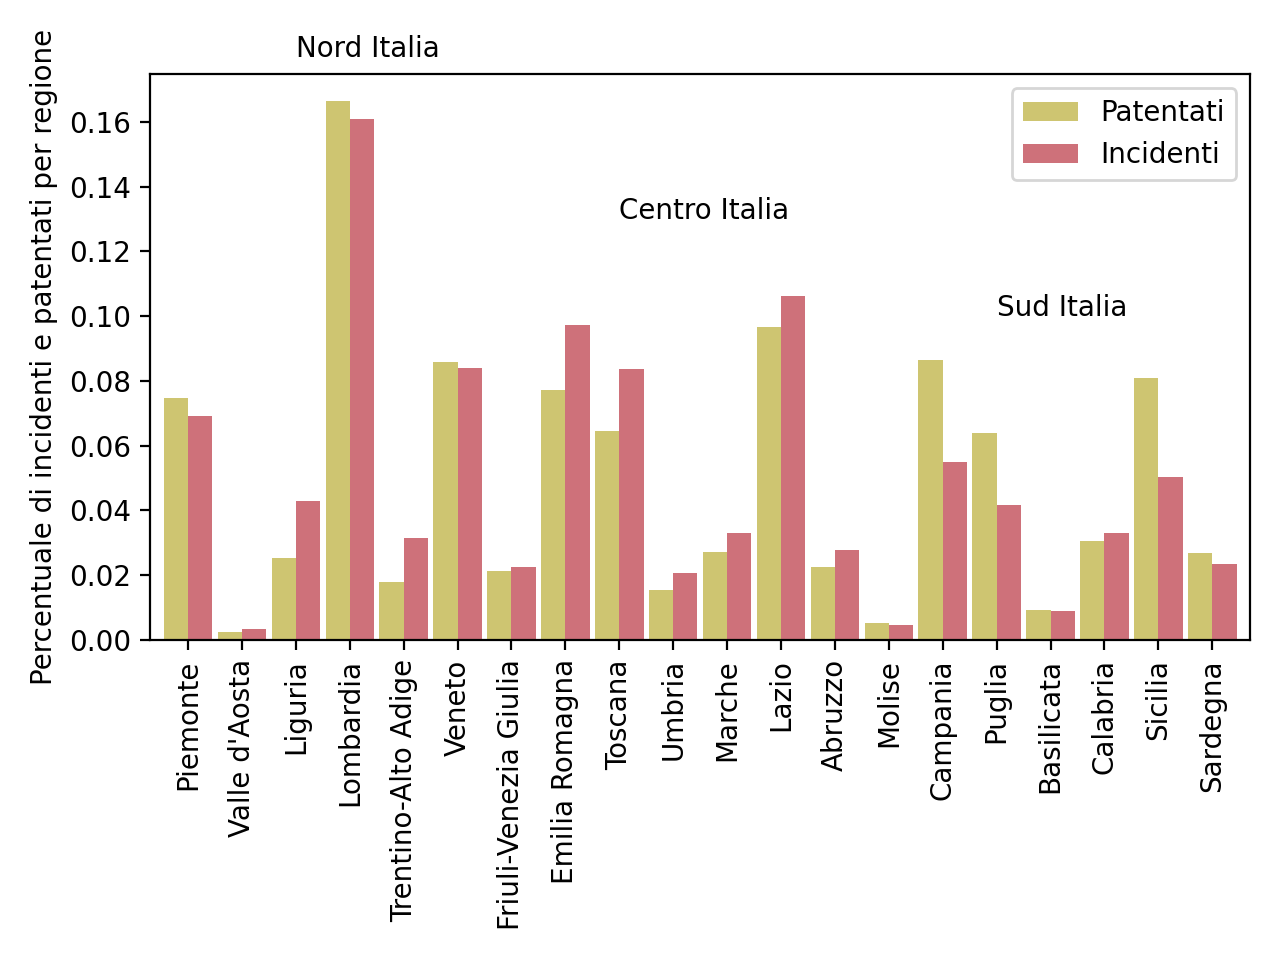
\includegraphics[width=0.7\linewidth]{../src/incidenti/incidenti_aci/mappe_regioni/incidenti_patenti_bar.png}\hspace*{\fill}
    \caption{Incidenti e patentati per regione}
    \label{fig:incidenti-patentati-bar}
\end{figure}

La figura \ref{fig:incidenti-patentati-box} permette di capire il motivo della disparità 
tra centro e Sud Italia. 
Al sud, la quantità di sinistri è molto minore rispetto al primo gruppo mentre, 
sempre nelle stesse due zone, il numero di patentati non cambia molto. 
\`E ovvio che tenendo il denominatore costante, il valore più basso di incidenti al 
sud porta come risultato a una frazione minore. 

\begin{figure}
    \hfill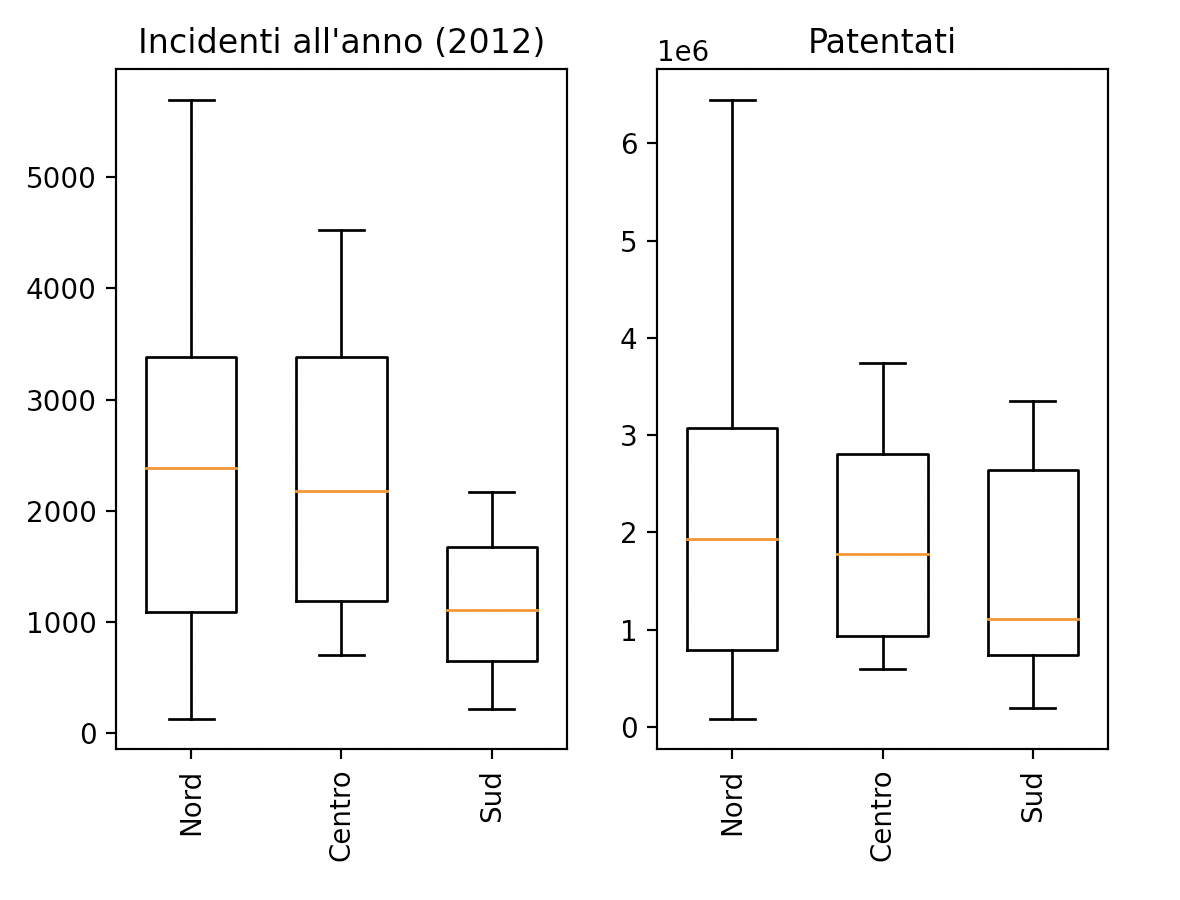
\includegraphics[width=0.7\linewidth]{../src/incidenti/incidenti_aci/mappe_regioni/incidenti_patenti_box.png}\hspace*{\fill}
    \caption{Incidenti e patentati per Nord, Centro e Sud Italia}
    \label{fig:incidenti-patentati-box}
\end{figure}

Quali potrebbero essere le motivazioni di questa disparità?
Come già accennato in precedenza, una delle ragioni principali 
potrebbe essere la destinazione lavorativa della popolazione, tuttavia, 
la precisione del numero di patenti come fattore utilizzato per la stima 
del traffico non è da considerarsi particolarmente attendibile. 

\subsection{Differenze di incidenti tra mesi estivi e invernali}
\todo{ATOK}

Sarebbe interessante verificare se i dati ACI confermano le tendenze trovate tramite 
le informazioni Istat, e vedere se nel Sud Italia, il numero di incidenti cresca 
come conseguenza delle vacanze estive. 

\begin{figure}
    \includegraphics[width=\linewidth]{../src/incidenti/incidenti_aci/mappe_regioni/estate_inverno.png}
    \caption{Incidenti per regione nei mesi estivi e invernali}
    \label{fig:estate-inverno}
\end{figure}

Nella figura \ref{fig:estate-inverno}, sono rappresentati i sinistri avvenuti 
in mesi invernali ed estivi, divisi per regione. 
In tutte le zone italiane, la quantità di incidenti in estate è maggiore di quella 
in inverno, e il comportamento ipotizzato non è visibile. 
La motivazione di ciò è probabilmente il fatto che 
le persone preferiscono muoversi meno nei mesi freddi rispetto a quelli caldi, 
anche in automobile. 

D'altra parte, un modo in cui si potrebbe tentare di ricavarlo, è osservare gli 
incidenti sulle autostrade principali in Agosto, su cui si muovono i turisti diretti 
nelle località marittime. 

Questo tipo di analisi verrà eseguita nei capitoli successivi. 

\subsection{Province italiane con maggior numero di incidenti}
\todo{ATOK}

Utilizzando ancora una volta, i file geojson trovati sul repository Github di 
Guglielmo Celata riguardanti le province, 
è possibile creare delle heatmap raffiguranti in quali, tra queste, siano 
presenti più incidenti. 
\todo{atrent: considerazione che vale un po' ovunque, attenzione che stai dando 
(a meno che non lo specifichi) valori assoluti, non in rapporto al traffico, 
alla popolazione, ai km di strade, ecc. tienilo sempre ben presente}

Avendo a disposizione dati riguardanti gli eventi lungo le strade provinciali e le autostrade, 
è stato realizzato lo stesso calcolo per entrambe le tipologie. 

\begin{figure}
    \includegraphics[width=\linewidth]{img_unite/lombardia_autostrade_provinciali.png}
    \caption{Incidenti sulle autostrade e strade provinciali in Lombardia}
    \label{fig:lombardia-strade}
\end{figure}

Nella figura \ref{fig:lombardia-strade} sono mostrati i sinistri in Lombardia, 
avvenuti rispettivamente sulle autostrade e nelle strade provinciali. 
In entrambi i casi, si nota che la provincia di Milano è quella caratterizzata da 
un maggior numero di incidenti. 
D'altra parte, per quanto riguarda le differenze, a Bergamo e Como, 
la quantità di sinistri cresce molto nella seconda categoria di strade osservata. 

Lo stesso calcolo è stato eseguito per le province del Lazio, visto che nel capitolo 
precedente sugli incidenti per regione, si era notata ampia disparità tra i due gruppi. 

\begin{figure}
    \includegraphics[width=\linewidth]{img_unite/lazio_autostrade_provinciali.png}
    \caption{Incidenti sulle autostrade e nelle strade provinciali nel Lazio}
    \label{fig:lazio-strade}
\end{figure}

Per quanto riguarda la figura \ref{fig:lazio-strade}, va 
specificato che il numero di sinistri su autostrade è molto più alto rispetto 
a quello sulle strade provinciali, fenomeno che, come anticipato, è stato osservato 
nella mappa \ref{fig:incidenti-per-regione}. 

Inoltre, la provincia di Frosinone ha un numero particolarmente alto di incidenti su 
autostrade, mentre quella di Latina, al contrario, ha un maggiore incremento di 
sinistri su strade provinciali. 

Non è difficile trovare il motivo di questo comportamento, in quanto l'autostrada A1 passa 
attraverso la prima provincia e non la seconda, e conseguentemente provoca 
un'impennata di valori nella heatmap di destra. 

%\clearpage
\subsection{Le strade in provincia di Milano con maggiore numero di incidenti}
\todo{ATOK}

Approfondendo le analisi del capitolo precedente, è possibile calcolare quali siano 
le strade più pericolose, concentrandosi sulla provincia di Milano. 
Il dataset ACI infatti fornisce il nome delle strade su cui sono avvenuti gli incidenti, 
tuttavia non presenta dati aggiuntivi sulla zona del sinistro, dunque per autostrade molto 
estese, questa misurazione potrebbe presentare errori di vari chilometri. 

Utilizzando il sito Geojson.io\footnote{\url{https://geojson.io/}}, 
è stato possibile tracciare i percorsi delle principali autostrade in prossimità di 
Milano, come le Tangenziali Est e Ovest, la Torino-Trieste e la A1. 
Il risultato è visibile nella figura \ref{fig:line-incidenti-milano}. 

\begin{figure}
    \includegraphics[width=\linewidth]{../src/incidenti/incidenti_aci/autostrade/incidenti_line_chart.png}
    \caption{Autostrade con più incidenti nel 2018}
    \label{fig:line-incidenti-milano}
\end{figure}

In particolare, dalla mappa \ref{fig:line-incidenti-milano}, si deduce che le 
Tangenziali Ovest e Est, e l'autostrada Torino-Trieste, sono i tratti di 
strada con maggior numero di incidenti, con più di $150$ all'anno. 

Infine, se si avessero a disposizione le coordinate precise degli incidenti, 
sarebbe possibile anche dividere queste tratte in sezioni più piccole, 
e verificare se esistano zone che alzano il volume di sinistri, e rendono queste strade 
più pericolose. 

%\clearpage
\subsection{Analisi della correlazione tra numero incidenti e numero di feriti}
\todo{ATOK}

Facendo uso dei dataset ACI a disposizione, è possibile stabilire l'esistenza di 
correlazione tra morti e incidenti, o tra morti e feriti?
Ovviamente ci si aspetta che la risposta a questa domanda abbia un 
esito positivo, poiché 
i campioni di feriti e morti sono strettamente collegati al numero di sinistri. 

L'indice di correlazione utilizzato è il coefficiente di Pearson, 
calcolato tramite la formula sottostante: 

\begin{center}
    $\rho_{X, Y} = \displaystyle \frac{cov(X, Y)}{\sigma_X \sigma_Y}$
\end{center}

\begin{center}
    con: $\rho_{X, Y} \rightarrow [-1, 1]$
\end{center}

Dove X e Y sono i due campioni tra cui si vuole calcolare la correlazione, 
\methodstyle{cov()} restituisce la covarianza, e $\sigma_X$ è la deviazione standard del 
campione X \cite{PROB_E_STATISTICA:1}. 

Una volta divisi i dati, è possibile calcolare l'indice tramite il metodo 
\methodstyle{corr()}, che restituisce un valore contenuto tra $-1$ e $1$. 
Se il numero si avvicina a uno, è possibile dire che tra i due campioni esista correlazione 
lineare, mentre la vicinanza all'altro estremo indica la presenza di correlazione inversa. 
I risultati del calcolo sono riportati nella tabella sottostante: 

\begin{center}
    \def\arraystretch{1.5}%  
    \begin{tabular}{ |c|c|c| } 
    \hline
    Incidenti & Incidenti & Feriti \\ 
    Feriti & Morti & Morti \\ 
    \hline
    0.9836 & 0.3385 & 0.3355 \\ 
    \hline
    \end{tabular}
\end{center}

\begin{figure}
    \includegraphics[width=\linewidth]{../src/incidenti/incidenti_aci/provincia/corr_incidenti.png}
    \caption{Correlazione tra numero di feriti e incidenti nelle venti province con maggior numero di sinistri}
    \label{fig:corr-incidenti-feriti}
\end{figure}

Tracciando il grafico \ref{fig:corr-incidenti-feriti}, contenente i primi trenta valori 
del dataset ACI, è chiaramente visibile la correlazione tra 
numero di incidenti e di feriti, in quanto, nella maggior parte dei casi, 
all'aumentare dei primi il volume dei secondi cresce allo stesso modo. 

Si è notato che, sia nel diagramma, sia nel dataset, il numero di feriti supera quello 
degli incidenti. 
Nella tabella sottostante è raffigurato un estratto del dataset ACI, 
di cui si sono prese in considerazione le colonne principali, più 
rilevanti per questo calcolo. 

\begin{center}
    \def\arraystretch{1.5}%  
    \begin{tabular}{ |c|c|c|c| } 
    \hline
    Provincia & Comune & Incidenti & Feriti \\ 
    \hline
    \rowcolor{TableGray}
    Torino & Brandizzo & 5 & 10\\
    Torino & Chivasso & 12 & 18\\
    \rowcolor{TableGray}
    Torino & Rondissone & 6 & 12\\
    Torino & Settimo Torinese & 25 & 40\\
    \hline
    \end{tabular}
\end{center}

Un'ipotesi, è che il dataset contenga solo incidenti con almeno un ferito, 
e quindi ignori tutti i sinistri non particolarmente significativi. 
D'altra parte, tenendo conto che si sono utilizzati dati raccolti lungo 
le autostrade, è anche possibile che la maggior parte degli eventi comporti 
un alto numero di infortunati, indubbiamente anche per la presenza di passeggeri a bordo.

Il coefficiente di Pearson, per quanto riguarda i campi \columnstyle{Incidenti} 
e \columnstyle{Feriti}, 
è molto vicino a uno, quindi i due campioni sono strettamente correlati. 

Correlazione, certo, non implica il nesso di causa e effetto, 
cioè, non è detto che due fattori correlati si influenzino in alcun modo,
ma sicuramente il variare del numero di sinistri nel dataset corrisponde 
a una variazione del numero di feriti.

I valori riguardanti i morti invece, sono molto meno vicini a uno, probabilmente 
per il minor numero di sinistri con esiti mortali, che rende il campione più ristretto. 

\subsection{Le autostrade italiane con maggior numero di incidenti}
\todo{ATOK}

Il dataset ACI raggruppa in un solo insieme sia le autostrade che le strade statali, 
esistono differenze sostanziali tra le due categorie? 

Essendo la densità veicolare sulle autostrade indubbiamente 
maggiore di quella sulle strade urbane, è possibile supporre che 
ciò renda le prime più pericolose delle seconde.

I file con incidenti 
localizzati\footnote{Per localizzati si intende che è stato riportato nel dataset 
il nome della strada in cui è avvenuto il sinistro}, 
possono permettere di verificare la correttezza dell'ipotesi, 
nonchè le differenze evidenziabili a parità di tipologia. 

\begin{figure}
    \includegraphics[width=\linewidth]{../src/incidenti/incidenti_aci/autostrade/autostrade.png}
    \caption{Autostrade e strade statali con più incidenti nel 2018}
    \label{fig:incidenti-autostrade}
\end{figure}
\todo{atrent: vale discorso assoluto/relativo}

Nella figura \ref{fig:incidenti-autostrade} sono  raffigurate le strade con 
maggiore numero di sinistri nel 2018. 
Non è una sorpresa che le prime posizioni della lista coincidano 
anche con le strade più trafficate, come l'Autostrada del Sole e l'Adriatica, 
tuttavia sono anche presenti, due strade statali, la SS1 e la SS16. 

La motivazione dell'alto numero di incidenti su queste direttrici, potrebbe essere 
la loro estensione. Infatti entrambe sono strade che corrono lungo tutta la 
penisola Italiana da nord a sud e, nella maggior parte delle tratte, 
hanno solamente due corsie. 

L'avere i sensi di marcia separati, e delle corsie designate al sorpasso, nel caso 
delle autostrade, non può che essere un fattore che influenza negativamente 
il numero degli incidenti. 
D'altra parte, l'essere costretti a sorpassare sulla corsia adibita al senso di 
marcia opposto, nel caso della SS1 e SS16, può portare ad un incremento dei 
sinistri. 

Purtroppo l'impossibilità di reperire dati precisi in merito, 
non consente di confutare le ipotesi con il dovuto grado di certezza.
Particolarmente utili sarebbero le coordinate di incidenti avvenuti lungo queste direttrici, 
in modo da poter individuare zone particolarmente pericolose.

\subsection{Analisi delle tratte pericolose lungo le principali strade statali}
\todo{ATOK}

Nonostante il dataset ACI non fornisca le coordinate geografiche degli incidenti avvenuti, 
un modo per aumentare la precisione dei dati a disposizione, potrebbe essere il 
ripartire i sinistri per provincia. 

Il procedimento è stato eseguito solo per le strade statali, 
ma per un'analisi più dettagliata di potrebbe estendere la verifica anche alle autostrade.

\begin{figure}
    \includegraphics[width=\linewidth]{img_unite/tratti_ss1_ss16.png}
    \caption{Incidenti su SS1 e SS16, divisi per provincia in cui questi sono avvenuti}
    \label{fig:incidenti-strade-statali}
\end{figure}

Il grafico sinistro della figura \ref{fig:incidenti-strade-statali}, 
contiene il numero di incidenti, oltre a quello di persone ferite, 
avvenuti in ogni provincia attraversata dalla SS1. 
Il tratto in cui avvengono più sinistri è quello prossimo a Savona, 
mentre le grandi città come 
Roma e Livorno hanno valori nella media o poco superiori. 

Lo stesso grafico, realizzato per la SS16, è rappresentato nella figura destra dell'immagine 
\ref{fig:incidenti-strade-statali}. 
In questo caso, il picco di sinistri avviene nella provincia 
di Bari, con quasi $200$ incidenti e $400$ feriti nel 2018. 

Una provincia che si differenzia vistosamente, per dei valori minori è quella di Pescara. 
Dopo aver eseguito il codice sottostante, tuttavia, si è osservato che tutte le righe 
del dataset per questa zona riportano valori uguali a zero, eccetto una. 

\begin{code}
data = pd.read_csv("dataset/incidenti/aci/autostrade/localizzazione_2018.csv")
ss16 = data[data['CODICE'] == 'SS01601']

pescara = ss16[ss16['PROVINCIA'] == 'Pescara'][['INC', 'FER']]
\end{code}

Controllando superficialmente i dati, si potrebbe essere portati a pensare 
che ci sia un errore di base nel conteggio dei valori. 
Del resto, considerando cha la SS16 in questa provincia non è molto lunga, 
può essere plausibile che durante l'anno sia avvenuto un solo incidente. 
A supporto i tale tesi, nella figura \ref{fig:ss16-pescara} si nota che questa direttrice, 
all'ingresso in città, diventi una strada urbana e molto probabilmente venga 
registrata con un altro nome.

\begin{figure}
    \hfill\includegraphics[width=0.7\linewidth]{img/pescara_ss16.png}\hspace*{\fill}
    \caption{La SS16 nella provincia di Pescara. All'ingresso in città questa strada cambia nome in SS714}
    \label{fig:ss16-pescara}
\end{figure}

Da un'analisi di questo tipo, non è facile trarre conclusioni approfondite 
o certe, data l'ampiezza della zona in cui può essere avvenuto il sinistro. 
Così pure il maggior numero di incidenti per provincia potrebbe essere dovuto 
semplicemente alla maggiore o minore estensione della strada nella 
provincia sotto osservazione. 
Inoltre, a eccezione di alcuni luoghi, come Bari, Savona, Viterbo e Massa-Carrara, 
la maggior parte degli incidenti sembrano essere omogeneamente distribuiti 
in tutte le colonne presenti nel grafico. 

Se si avesse a disposizione la lunghezza delle due strade statali, 
divisa per ogni provincia attraversata,
o anche il flusso di automobili nei luoghi in questione, 
si potrebbe verificare l'esistenza di tratti particolarmente pericolosi. 

\subsection{Le autostrade con più incidenti cambiano di anno in anno?}
\todo{ATOK}

Tornando a concentrarsi sui dati riguardanti le autostrade, 
sarebbe interessante sapere ci sia una variazione di incidenti con il trascorrere degli anni. 
Una motivazione di questo fenomeno potrebbe essere il cambiamento 
delle località di vacanza preferite. 
Nel 2018, le mete più frequentate sono state Puglia e 
Toscana \cite{INFOGRAFICA_ISTAT:1}, mentre nel 2019, oltre alla Puglia, 
una percentuale sostanziale di turisti si è recata in 
Emilia Romagna e Liguria \cite{REPORT_ISTAT_2019:1}. 
\todo{lelepado: è giusto lo spazio tra parola e citazione?}

Avendo a disposizione i dati di tutte le annate, a partire dal 2010 fino al 2018, 
è possibile verificare se esistano anni con un volume di 
sinistri in Agosto particolarmente alto. 

\begin{figure}
    \includegraphics[width=\linewidth]{../src/incidenti/incidenti_aci/agosto/vacanze_autostrade.png}
    \caption{Incidenti in strade per anno nel mese di Agosto}
    \label{fig:autostrade-anno}
\end{figure}

Controllando le prime cinque direttrici per incidentalità in ogni anno, 
raffigurate nella heatmap \ref{fig:autostrade-anno}, si ottiene 
un risultato decisamente definito, vista la ripetizione delle medesime 
tratte ai vertici della classifica.
\todo{lelepado: i termini inglesi vanno messi in corsivo?}

La strada statale Adriatica è sempre in prima posizione, con una media di $171.5$ 
sinistri nel mese di Agosto. 
Le posizioni successive invece cambiano a seconda dell'anno, in particolare però, 
nell'autostrada A4 (Torino-Trieste) il numero di incidenti è progressivamente cresciuto, 
evento imputabile alla nuova popolarità delle vacanze in montagna anche nel periodo estivo. 

Utilizzando il dataset Istat riguardante il turismo in Italia, e in 
particolare sfruttando due indicatori, Tasso di 
Turisticità\footnote{Tasso di Turisticità: indica il numero di turisti 
presenti ogni 100.000 abitanti\cite{ONTIT:1}} 
e turismo in mesi non estivi, è stato possibile realizzare 
la figura \ref{fig:turismo}, 
contenente i valori di questi, nel periodo a partire dall'anno 1995 fino al 2018. 

\begin{figure}
    \includegraphics[width=\linewidth]{../src/turismo/turismo.png}
    \caption{Turismo nelle principali località estive e invernali}
    \label{fig:turismo}
\end{figure}

Nel grafico \ref{fig:turismo} sono state incluse alcune regioni con località popolari 
durante le vacanze estive, come Sardegna, Sicilia e Liguria, e altre, principalmente 
di montagna, come Trentino e Valle d'Aosta. 
La Lombardia, infine, è stata aggiunta per assicurarsi che il comportamento delle due zone 
di alpine non fosse comune a tutto il Nord Italia. 

Ciò che si può concludere, oltre al fatto che le zone di montagna abbiano 
un tasso di turisticità particolarmente alto, rapportato al minor numero di residenti,
è che, a partire dal 2015, sia presente una crescita nel volume di turisti nelle località 
del Nord Italia a eccezione della Lombardia, e che questo incremento non è visibile nelle 
destinazioni marittime. 

In particolare, rispetto al 2015, in Trentino nel 2018 si ha un aumento 
di turisti del $11.9$ \%, mentre rispetto alla 
media\footnote{Calcolata sull'insieme di anni disponibili, quindi 
a partire dal 1995 fino al 2018} l'aumento è del $14.7$ \%. 

In Valle d'Aosta, allo stesso modo, l'incremento di turisti nel 2018 
rispetto al 2015 è del $13$ \%, mentre scende al $7.6$ \% rispetto alla media annuale. 

Occorre evidenziare, infine, che non è possibile stabilire una relazione 
tra la crescita di popolarità delle zone montane, 
con l'aumento di incidenti sull'autostrada Torino-Trieste. 
Il numero di sinistri, infatti rimane sostanzialmente costante negli anni analizzati, 
variando da $99$ incidenti nel 2011 a $97$ nel 2018. 

\subsection{Differenze di incidenti su autostrade in base al mese dell'anno}
\todo{ATOK}

Una questione, di cui ci si è occupati tramite dati Istat in precedenza, è 
quella dei mesi con maggiore incidentalità. 
Il dataset ACI permette di individuare gli stessi cambiamenti di tendenza rilevati nei 
capitoli precedenti, aggiungendo la discrimina della tipologia di strada. 

In particolare, nell'analisi precedente si era individuato un decremento di valori 
nei mesi estivi nella provincia di Milano, e il comportamento opposto a 
Rimini e Aosta. 

\begin{figure}
    \includegraphics[width=\linewidth]{../src/incidenti/incidenti_aci/autostrade/mesi_autostrade.png}
    \caption{Incidenti per mese nel 2018}
    \label{fig:incidenti-per-mese}
\end{figure}

La heatmap \ref{fig:incidenti-per-mese} mostra che su alcune autostrade, come il 
Grande Raccordo Anulare a Roma, il numero di incidenti diminuisce durante i mesi 
estivi. 
D'altra parte, la tendenza opposta avviene sulla A1 e la A4, 
con picchi di sinistri in Giugno e Luglio per, come precedentemente ipotizzato, 
l'aumento di traffico dovuto alle partenze per le vacanze. 
Sull'Adriatica e sull'Aurelia infine, prevalgono eventi 
in Luglio e Agosto e in generale nei mesi estivi. 

\begin{figure}
    \hfill\includegraphics[width=0.7\linewidth]{../src/incidenti/incidenti_aci/autostrade/adriatica_roma.png}\hspace*{\fill}
    \caption{Incidenti sull'Adriatica e sul Grande Raccordo Anulare a Roma nel 2018}
    \label{fig:adriatica-roma}
\end{figure}

Isolando gli incidenti avvenuti sul Grande Raccordo Anulare a Roma, e quelli avvenuti 
sull'Adriatica, raffigurati nel grafico \ref{fig:adriatica-roma}, si osserva, 
nel primo caso, un numero di sinistri per mese molto omogeneo, a eccezione di 
Agosto, quando si rileva un calo del $46$ \% rispetto alla media mensile. 
D'altra parte, nel caso dell'Adriatica, è presente una campana con apice nei 
mesi di Luglio e Agosto, comportamento opposto a quello sull'autostrada 
romana. 

L'analisi si conclude quindi asserendo che l'incidentalità sicuramente subisce 
variazioni anche profonde, in base alla stagionalità, ma certo le variabili 
che intervengono sono tante, la maggior parte delle quali sono
a loro volta influenzate dal trascorrere dei mesi.

%\clearpage%
\subsection{Analisi degli incidenti in orari di punta su autostrade}
\todo{ATOK}

Rimanendo sull'argomento delle analisi già eseguite con i dati Istat, 
si potrebbe replicare, con i dataset ACI, quella riguardante gli orari di incidenti. 
Avendo a disposizione il nome della strada, è anche possibile selezionare delle zone precise 
su cui avvengono molti sinistri, come la SS1 e SS16. 

\begin{figure}
    \includegraphics[width=\linewidth]{../src/incidenti/incidenti_aci/orari/orari.png}
    \caption{Incidenti all'anno per orario su strade e località italiane diverse}
    \label{fig:orari-strade-aci}
\end{figure}

Negli istogrammi in figura \ref{fig:orari-strade-aci} sono rappresentati 
gli incidenti avvenuti 
nel 2018, divisi per orario, sulla SS16 Adriatica in provincia di Bari, sulla SS1 
a Genova, e infine sul Grande Raccordo Anulare a 
Roma\footnote{Si sono prese in considerazione delle zone, distanti tra loro, 
con dimensione del campione significativa.}. 

Le tendenze visibili nei tre grafici sono molto simili tra loro. 
A Roma in particolare, dove si ha maggiore 
volume di sinistri, si osservano picchi nelle fasce orarie delle 
7:00-9:00 e delle 17:00-19:00, già evidenziate nei capitoli precedenti sull'argomento. 

Prendendo in considerazione invece, la provincia di Milano, si potrebbero ricavare 
informazioni interessanti su quali siano le strade più utilizzate per 
andare e tornare dai luoghi di lavoro. 

\begin{figure}
    \includegraphics[width=\linewidth]{../src/incidenti/incidenti_aci/orari/tangenziali_autostrade.png}
    \caption{Incidenti nelle principali autostrade di Milano per orario}
    \label{fig:tangenziali-autostrade}
\end{figure}

La heatmap \ref{fig:tangenziali-autostrade} conferma, per alcune autostrade, 
l'esistenza di picchi di incidenti durante gli orari di punta ad esempio, 
sulla A4 Torino-Trieste, 
per la Tangenziale Ovest e per la Tangenziale Est. 

\`E possibile ipotizzare che queste siano le strade più utilizzate per 
raggiungere i luoghi di lavoro? 

Certamente la maggior parte dei residenti a Milano non utilizzerà le tratte incluse 
nell'ultimo grafico, poiché essendo già a Milano, 
viaggeranno lungo le direttrici urbane, o utilizzando i mezzi pubblici. 
Tuttavia, per quanto riguarda i pendolari, è molto probabile che, quelli provenienti 
da nord, ad esempio da Varese, Busto Arsizio o Novara, 
facciano uso della Tangenziale Ovest, 
e dunque siano registrati nei conteggi. 

Questa stima, di certo, non permette di affermare con sicurezza 
che la maggior parte dei pendolari utilizzino le strade prese in considerazione 
nei grafi, 
tuttavia, gli incidenti durante le ore di punta sulle autostrade A4 e sulle 
Tangenziali sono particolarmente frequenti e, avendo a disposizione dati più 
precisi, per esempio sulle tratte percorse dai pendolari, sarebbe possibile 
realizzare analisi più approfondite. 

%\clearpage
\subsection{Annate con maggior numero di incidenti su autostrade}
\todo{ATOK}

Nel capitolo precedente si è tentato di individuare quali strade siano maggiormente 
utilizzate per recarsi a lavoro a Milano. 
Sarebbe interessante realizzare un calcolo simile, per quanto riguarda le autostrade 
più percorse per spostarsi in località di vacanza. 

Sicuramente il mese di Agosto è quello interessato dal maggior numero 
di partenze per le località di villeggiatura e sicuramente l'intenzione 
di chi si sposta in automobile è quella di spostarsi verso sud, 
e raggiungere le zone balneari. 

\begin{figure}
    \includegraphics[width=\linewidth]{../src/incidenti/incidenti_aci/agosto/autostrade_anno_agosto.png}
    \caption{Autostrade con più incidenti per anno, in Agosto}
    \label{fig:autostrade-anno-agosto}
\end{figure}

Nell'istogramma \ref{fig:autostrade-anno-agosto} sono elencate le 
autostrade su cui sono avvenuti più incidenti nel mese di Agosto, per annata. 
In questo grafico, si è tentato un approccio diverso rispetto a quello del capitolo precedente, 
elencando le strade più pericolose in base all'anno e al numero di sinistri, invece di usare una 
heatmap, come nella figura \ref{fig:autostrade-anno}. 

La colorazione delle colonne, nel grafico \ref{fig:autostrade-anno-agosto}, è stata aggiunta per 
facilitare la lettura delle direttrici, infatti a colori diversi corrispondono tratte diverse. 

In particolare emergono la SS16 Adriatica e SS1 Aurelia che, come già 
detto in precedenza, essendo strade statali molto lunghe e con corsie di marcia 
non separate, potrebbero risultare più pericolose rispetto alle autostrade. 
A questo si deve poi aggiungere l'attraversamento di diversi centri urbani, 
che certo aumenta la possibilità di incidenti. 

\`E anche curioso che le uniche autostrade presenti nel grafico siano la A1 e la A14, 
solamente in occasione dell'estate 2011. 
Ciò è dovuto al fatto che, in ogni annata, le strade nelle prime posizioni per incidenti sono 
quelle statali citate in precedenza, e solo in alcune occasioni il numero di sinistri 
nelle autostrade è sufficiente a garantire un posto nell'istogramma. 

\section{Meteo a Milano}

\subsection{Analisi sulla correlazione tra fattori atmosferici e incidentalità}
\todo{Da leggere}

Ipotizzare che esista correlazione tra le condizioni meteo e il numero di incidenti, 
può non sembrare improponibile, tuttavia i valori necessari a quantificare una stima
di tale interdipendenza, sono inesistenti a livello di dati liberi.

Un esempio dei dataset richiesti potrebbe essere, conoscere il giorno e l'ora 
dell'incidente, e allo stesso modo anche le zone in cui si sono verificati determinati 
fenomeni atmosferici, come nevicate abbondanti o temporali violenti. 
Entrambi i dati non sono disponibili tramite i siti utilizzati finora e, 
probabilmente, anche assumendo l'esistenza di questi non sarebbe possibile dare una 
buona stima della correlazione tra i due fattori. 

\`E comunque interessante mostrare come, il coefficiente di Pearson tra due campioni 
possa essere estremamente alto, anche se questi ultimi sono completamente scollegati. 

\begin{figure}
    \includegraphics[width=\linewidth]{img_unite/temp_incidenti.png}
    \caption{Incidenti, temperature e umidità medi per mese nel 2011 e nel 2013}
    \label{fig:incidenti-temp}
\end{figure}

La figura \ref{fig:incidenti-temp} mostra, partendo dall'alto, il numero di sinistri 
avvenuti per mese, la temperatura media mensile, e infine l'umidità. 
Sono state riportate le due annate con rispettivamente la maggiore e la minore correlazione tra 
incidenti e fattori atmosferici. 

Non è stato possibile eseguire la stessa operazione con dati più recenti, per mancanza del 
campo \columnstyle{mese}, convertito in \columnstyle{trimestre} a partire dal 2014. 
I risultati sono riportati nella tabella sottostante: 

\begin{center}
    \def\arraystretch{1.5}%  
    \begin{tabular}{ |c|c|c|c| } 
    \hline
    Anno & Temperatura & Velocità del Vento & Umidità \\ 
    \hline
    \rowcolor{TableGray}
    2010 & 0.768 & 0.585 & -0.626 \\
    2011 & 0.900 & 0.626 & -0.730 \\
    \rowcolor{TableGray}
    2012 & 0.732 & 0.501 & -0.609 \\
    2013 & 0.658 & 0.465 & -0.516 \\
    \hline
    \end{tabular}
\end{center}

Per le annate a disposizione, i dati sono consistenti tra loro, e indicano la presenza di 
correlazione lineare tra temperatura e sinistri, mentre si ha dipendenza inversa per quanto 
riguarda l'umidità. 

Ciò non significa che, nel 2011, sia stata l'alta temperatura a provocare 
tutti gli incidenti, anzi, è molto più probabile che il fattore determinante 
sia proprio il mese, e non invece l'umidità o la velocità del vento. 

Infatti, il dataset sulle condizioni meteo che si sta utilizzando è molto impreciso, 
in quanto potrebbero esserci differenze di diversi gradi, in zone lontane di Milano. 
Allo stesso modo, anche i dati sugli incidenti non sono particolarmente definiti, 
visto che indicano solo il nome dell'autostrada in cui è avvenuto 
il sinistro, e la posizione effettiva potrebbe essere a chilometri di distanza da dove 
si è calcolata l'informazione sul clima. 

Dal punto di vista, invece, della velocità del vento, sarebbe possibile eseguire 
un'analisi più approfondita, in quanto un valore del coefficiente di Pearson uguale 
a $0.5$ non è particolarmente alto. 
Si potrebbe, per esempio, verificare se esista una qualche differenza tra gli 
incidenti su moto rispetto a quelli in automobile; 
oppure, avendo a disposizione la velocità del vento all'uscita delle gallerie, 
analizzare la quantità di sinistri in queste zone, notoriamente pericolose 
in presenza di forti correnti d'aria improvvise. 

Infine, osservando le misurazioni sull'umidità, è possibile ipotizzare 
in questo caso la presenza di un rapporto di causa e effetto, 
in quanto spesso, un valore alto di questo fattore 
coincide con pioggia e temporali, che a loro volta rendono più difficoltosa la guida. 

\chapter{Conclusioni}
\todo{ATOK}

Riprendendo alcune delle analisi realizzate in questo lavoro, è opportuno dire che buona 
parte di queste sono state portate a termine con compromessi 
tra la disponibilità di un dato e la sua precisione ed attendibilità.

In particolare, i capitoli che fanno utilizzo dei dati localizzati, soffrono la mancanza di 
queste informazioni per annate diverse dal 
2016\footnote{Il dataset con le coordinate degli incidenti è disponibile solo per l'anno 2016}, 
come si è potuto osservare nella sezione riguardante gli autovelox. 

Le analisi dei dataset Istat e Aci, invece, facendo uso di informazioni già aggregate 
e di facile elaborazione, sono state portate a termine con maggiore 
accuratezza, e il principale ostacolo è stato il creare un contesto 
corretto attorno ai risultati ottenuti. 

\`E, per esempio, il caso dei sinistri divisi per età della popolazione, 
dove si sono ottenuti esiti 
molto diversi a seconda di quali percentuali venivano usate per stimare la quantità di 
persone in ogni fascia. 

\skipline
Per concludere, sarebbe opportuno riportare quali siano state le maggiori difficoltà 
incontrate durante l'analisi di dati liberi appena realizzata. 

Uno dei problemi riscontrati, soprattutto per quanto riguarda il confermare la 
validità dei risultati calcolati, è stata la mancanza di dataset 
inerenti la mole di traffico e la tipologia di fondo stradale.

Nel capitolo riguardante gli autovelox infatti, non è stato possibile individuare 
un comportamento precedente all'installazione delle telecamere, cioè prima dell'anno 2016, 
per la mancanza di informazioni sulla posizione precisa dei sinistri. 

Per ovviare a queste difficoltà si è spesso dovuto ricorrere a stime, 
come il numero di accessi in area C. 
L'assenza di informazioni ha giocato un ruolo anche nelle analisi riguardanti gli incroci, 
in quanto non si sono trovati riferimenti al totale di questi in alcun sito di open data, 
anche tentando di restringere il campo di ricerca a singole città. 


In secondo luogo, alcuni dataset non sono completi, o hanno sezioni temporali mancanti. 
\`E il caso delle informazioni sugli ingressi all'area C di Milano dove, 
per il 2013 non è presente il mese di Dicembre. 

Rimanendo sull'argomento, lo stesso dataset, a partire dal 2017, è disponibile 
solamente diviso in dodici file su base mensile. 
Questo, in passato, era un comportamento ricorrente, in 
quanto molte piattaforme, come quella del Ministero dei 
Trasporti\footnote{\url{http://dati.mit.gov.it/catalog/dataset}}, 
misuravano le condivisioni di open data delle istituzioni 
sulla base del numero di documenti pubblicati. 
Era quindi più proficuo condividere dati separati, rispetto a tutte le informazioni in 
un unico dataset. 

Ovviamente questa operazione rende non solo la raccolta delle informazioni più complessa, 
ma anche l'associazione di queste, che magari sono presenti in un file e non in un altro. 
Il sito Global Open Data Index, che offre un punteggio in base a quanti dati ogni paese 
ha condiviso in formato libero, nelle metodologie di calcolo della classifica, scrive: 

\begin{quotation}
    \dots we expect that national governments also provide aggregation 
    of that data from 
    sub governments so as to ensure users have an easy way to access use the data 
    (the best solution is one consolidated dataset but at a minimum could consist of a 
    single point of access to all data subsets).\cite{OPENDATAINDEX:1}
\end{quotation}

\begin{quotation}
    \dots Ci si aspetta che i governi nazionali provvedano per 
    l'aggregazione dei dati provenienti dalle 'regioni', per garantire agli utenti 
    un punto di accesso 
    alle informazioni (la soluzione migliore sarebbe l'avere un dataset unico, ma è sufficiente 
    avere un solo punto di accesso a tutti i sottoinsiemi di dati). 
\end{quotation}

\skipline
Infine, una problematica riscontrata con frequenza è stata la mancanza 
di uno standard per quanto riguarda la nomenclatura delle colonne. 
Le tabelle provenienti dal sito Istat, per esempio, nel 2011, hanno un campo denominato 
\columnstyle{intersezione\_o\_non\_interse1}, 
mentre nel 2018, la stessa informazione prende il nome di 
\columnstyle{intersezione\_o\_non\_interse3}.
\todo{lelepado: risolto così l'uscita delle parole dai margini}

A cambiare non sono soltanto i nomi delle colonne negli anni, 
ma in alcuni casi, nei label, viene usato un solo \quotestyle{underscore} a 
simboleggiare uno spazio, mentre nel campo\\
\indent\columnstyle{veicolo\_\_a\_\_\_et\_\_conducente}\\
ne sono usati due o anche tre. 

Rimanendo in tema, lo stesso dataset Istat ha colonne con differenze di anno in anno, 
come \columnstyle{mese}, che è presente fino al 2013, e successivamente viene 
sostituito dal campo \columnstyle{trimestre}. 
In questo caso, non solo è presente un cambio di nomenclatura, ma il dato in sè è 
anche reso più vago. 

\chapter{Utilizzo del Codice}
\todo{ATOK}

Tutti gli script utilizzati per questo lavoro sono reperibili a questa pagina 
github: \url{https://github.com/lelepado01/Tirocinio}. 

Il repository è diviso in tre cartelle principali, \filenamestyle{dataset}, \filenamestyle{src} 
e \filenamestyle{tesi}. La prima contiene tutti i file di dati utilizzati, divisi per 
argomento, e alcuni documenti di testo riguardanti le stime realizzate, come la percentuale di 
conducenti maschio e femmina. 

La cartella \columnstyle{tesi}
\todo{atrent: io questo columnstyle lo vedo identico al resto lelepado: in che senso? 
io lo vedo con font typewriter} contiene la maggior parte delle immagini presenti 
nella relazione\footnote{Ci si riferisce alle figure ottenute tramite screenshot 
da Google Maps e altri siti, non ai grafi.} 
e il codice sorgente \LaTeX usato per produrre questo documento.

Infine, nella directory \filenamestyle{src} è contenuto il codice sorgente utilizzato 
per realizzare i grafi, le mappe e le stime, diviso per argomento. 
Ogni grafico è associato a uno script python che ne permette la creazione, registrato con 
lo stesso nome, e estensione \filenamestyle{.py}. 

Quindi se in una cartella fosse presente l'immagine \filenamestyle{esempio.png}, lo script con 
cui questa è stata creata avrà nome \filenamestyle{esempio.py}. 

Invece, se si volessero trovare le informazioni sul grafico raffigurante 
l'incremento di incidenti dal 2010 al 2018, i dataset utilizzati si troverebbero 
nella directory:

\skipline
\indent\filenamestyle{dataset/incidenti/incidenti\_istat}

\skipline
\noindent Mentre il codice sorgente e le immagini sarebbero situati al percorso:

\skipline
\indent\filenamestyle{src/incidenti/incidenti\_senza\_coords/anno}

\skipline
Alcune figure, in particolare quelle con grafici posizionati in coppia 
orizzontalmente\footnote{I grafici singoli sono tutti nella directory \filenamestyle{src}, 
le figure doppie, unite tramite programmi esterni, in più, sono raccolte separatamente 
in \filenamestyle{tesi/img\_unite}}, 
sono raccolte nella cartella \filenamestyle{tesi/img\_unite}, 
mentre la directory \filenamestyle{tesi/img} contiene gli screenshot 
che non hanno bisogno di codice sorgente. 

Infine, in modo da fornire un collegamento tra i dataset nella specifica cartella e i siti 
di open data in cui sono stati trovati, nella tabella sottostante sono associati i percorsi di 
ogni file e l'url del portale di origine. 

\begin{center}
    \def\arraystretch{1.5}%  
    \begin{tabular}{ |c|c| } 
    \hline
    Percorso Cartella & Fonte \\ 
    \hline
    \rowcolor{TableGray}
    dataset/area\_c & Comune di Milano\footnotemark[1] \\
    dataset/atm & Comune di Milano\footnotemark[2] \\
    \rowcolor{TableGray}
    dataset/autovelox & OpenStreetMaps\footnotemark[3] \\
    dataset/incidenti/aci/autostrade & Portale ACI\footnotemark[4] \\
    \rowcolor{TableGray}
    dataset/incidenti/aci/strade\_provinciali & Portale ACI\footnotemark[5] \\
    dataset/incidenti/istat & Archivio Istat\footnotemark[5]\\
    \rowcolor{TableGray}
    dataset/incidenti & TheSubmarine\footnotemark[7]\\
    dataset/manto\_stradale\_milano & Geoportale Milano\footnotemark[8]\\
    \rowcolor{TableGray}
    dataset/meteo & Zenodo\footnotemark[9]\\
    dataset/milano\_municipi & Geoportale Milano\footnotemark[10]\\
    \rowcolor{TableGray}
    dataset/patenti & Ministero dei Trasporti\footnotemark[11]\\
    dataset/pave/tram & Geoportale Milano\footnotemark[12]\\
    \rowcolor{TableGray}
    dataset/regioni & Github\footnotemark[13]\\
    dataset/turismo & Archivio Istat\footnotemark[14]\\
    \hline
    \end{tabular}
\end{center}

\footnotetext[1]{\url{https://dati.comune.milano.it/dataset?tags=Area+C}}
\footnotetext[2]{\url{https://dati.comune.milano.it/dataset/ds538_atm-percorsi-linee-di-superficie-urbane}}
\footnotetext[3]{\url{https://www.openstreetmap.org/}}
\footnotetext[4]{\url{http://www.aci.it/fileadmin/documenti/ACI/Trasparenza/Open_Data/Catalogo_localizzazione_in_formato_Open_2019.pdf}}
\footnotetext[5]{\url{http://www.aci.it/fileadmin/documenti/ACI/Trasparenza/Open_Data/Old_A_LOCALIZZAZIONE_INCIDENTI_STRADALI_STRADE_PROVINCIA.pdf}}
\footnotetext[6]{\url{https://www.istat.it/it/archivio/87539}}
\footnotetext[7]{\url{https://thesubmarine.it/2018/06/20/mappa-incidenti-stradali-milano/}}
\footnotetext[8]{\url{https://geoportale.comune.milano.it/ATOM/SIT/DBT2012/DBT2012_STRATO_01_Dataset_1.xml}}
\footnotetext[9]{\url{https://zenodo.org/record/3992354}}
\footnotetext[10]{\url{https://geoportale.comune.milano.it/ATOM/SIT/Municipi/Municipi_Dataset_1.xml}}
\footnotetext[11]{\url{https://www.mit.gov.it/sites/default/files/media/notizia/2017-07/INFOGRAFICA Dati sintesi patenti Italia.pdf}}
\footnotetext[12]{\url{https://geoportale.comune.milano.it/ATOM/SIT/DBT2012/DBT2012_STRATO_01_Dataset_1.xml}}
\footnotetext[13]{\url{https://github.com/openpolis/geojson-italy}}
\footnotetext[14]{\url{https://www.istat.it/it/archivio/16777}}


%\addcontentsline{toc}{chapter}{Bibliografia}
\printbibliography

\end{document}
